%  ========================================================================
%  Copyright (c) 1985 The University of Washington
%
%  Licensed under the Apache License, Version 2.0 (the "License");
%  you may not use this file except in compliance with the License.
%  You may obtain a copy of the License at
%
%      http://www.apache.org/licenses/LICENSE-2.0
%
%  Unless required by applicable law or agreed to in writing, software
%  distributed under the License is distributed on an "AS IS" BASIS,
%  WITHOUT WARRANTIES OR CONDITIONS OF ANY KIND, either express or implied.
%  See the License for the specific language governing permissions and
%  limitations under the License.
%  ========================================================================
%

% Documentation for University of Washington thesis LaTeX document class
% by Jim Fox
% fox@washington.edu
%
%    Revised 2020/02/24, added \caption()[]{} option.  No ToC.
%
%    Revised for version 2015/03/03 of uwthesis.cls
%    Revised, 2016/11/22, for cleanup of sample copyright and title pages
%
%    This document is contained in a single file ONLY because
%    I wanted to be able to distribute it easily.  A real thesis ought
%    to be contained on many files (e.g., one for each chapter, at least).
%
%    To help you identify the files and sections in this large file
%    I use the string '==========' to identify new files.
%
%    To help you ignore the unusual things I do with this sample document
%    I try to use the notation
%       
%    % --- sample stuff only -----
%    special stuff for my document, but you don't need it in your thesis
%    % --- end-of-sample-stuff ---


%    Printed in twoside style now that that's allowed
%
 
\documentclass [11pt, proquest] {uwthesis}[2020/02/24]
 
%
% The following line would print the thesis in a postscript font 

% \usepackage{natbib}
% \def\bibpreamble{\protect\addcontentsline{toc}{chapter}{Bibliography}}

\setcounter{tocdepth}{1}  % Print the chapter and sections to the toc

% ==========   Local defs and mods
%

\usepackage[utf8]{inputenc}
\usepackage{csquotes}
\usepackage[english]{babel}

\usepackage[style=apa, apamaxprtauth=99]{biblatex}

% Remove eprint URLs that don't format correctly.
\DeclareSourcemap{
    \maps[datatype=bibtex]{
        \map{
            \step[fieldset=eprint, null]
        }
    }
}

\addbibresource{uwthesis.bib}

\usepackage{graphicx}

\usepackage[binary-units=true]{siunitx}
\sisetup{per-mode=symbol-or-fraction}
\DeclareSIUnit\month{mo}
\DeclareSIUnit\millibar{mb}

\usepackage{amsmath}

\begin{document}
 
% ==========   Preliminary pages
%
% ( revised 2012 for electronic submission )
%

\prelimpages
 
%
% ----- copyright and title pages
%
\Title{Time Step Sensitivity and Process Coupling in Climate Models}
\Author{Sean Patrick Santos}
\Year{2020}
\Program{Applied Mathematics}

\Chair{Christopher S. Bretherton}{Professor}{Department of Applied Mathematics and Department of Atmospheric Sciences}
\Signature{Peter M. Caldwell}
\Signature{Randall J. LeVeque}

\titlepage

\newpage

\copyrightpage

 
%
% ----- signature and quoteslip are gone
%

%
% ----- abstract
%


\setcounter{page}{-1}
\abstract{%
  Time integration in climate models is complex, typically involving several levels of nested sets of substepped processes, potentially using a different time integration scheme at each level. Many climate models are also subject to a high degree of time step sensitivity, producing a significantly different climate when the model's time step is reduced. In order to reduce the effect of time integration error on model output, it is therefore important to attribute a model's time step sensitivity to particular processes or sets of processes in need of improvement. This study focuses on attributing time step sensitivity to sets of processes in the Energy Exascale Earth System Model version 1 (E3SMv1), and in particular in E3SMv1's atmosphere model (EAMv1).
  
  The first stage of this study focuses on EAMv1's stratiform microphysics scheme, the Morrison-Gettelman microphysics version 2 (MG2). Numerically relevant timescales in MG2 are derived by computing the eigenspectrum of its Jacobian. These timescales are found to often be smaller than the default 5 min time step used for MG2. The fast timescales are then heuristically connected to individual microphysics processes. By substepping a few particular rain processes within MG2, the time discretization error for those processes was considerably reduced with minimal additional expense to the overall microphysics. While this improvement has a substantial effect on the target processes and on the vertical distribution of stratiform‐derived rain within EAMv1, the overall model climate is found to not be sensitive to the MG2 time step alone.
  
  The second stage of this study examines E3SM as a whole. We find significant time step sensitivity in EAMv1, leading to large decreases in the magnitude of cloud forcing when the time step is reduced to 10 seconds. When MG2 is substepped together with other cloud physics processes, the effect of MG2 substepping is amplified, causing increased precipitation, a drying of the atmosphere, and an increase in surface evaporation. Coupling the model’s dynamics and physics more frequently reduces cloud fraction at lower altitudes, while producing more cloud liquid at higher altitudes. Reducing the deep convection time step also reduces low cloud mass and cloud fraction.
  
  We conclude that the cloud physics in a global circulation model can depend strongly on time step, and particularly on the frequency with which cloud-related processes are coupled with each other and with the model dynamics. Substepping individual processes often seems to be an attractive method for improving time integration without excessive computational cost. However, substepping can easily fail to reproduce the effect of changing the entire time step for a model. Effective use of substepping therefore requires careful analysis to group processes that jointly contribute to a model's time step sensitivity.
}

%
% ----- contents & etc.
%
\tableofcontents
\listoffigures
\listoftables
 
%
% ----- acknowledgments
%
\acknowledgments{% \vskip2pc
  % {\narrower\noindent
  I must express my heartfelt gratitude to my advisors, Peter Caldwell and Chris Bretherton, whose support and guidance have been an indispensable resource during this project. In particular, Peter's interest in a more rigorous analysis of the MG2 microphysics was the seed that grew into this entire study. I've been thankful for their positive interest and new ideas that inspired me, and for their (very) patient work nudging me back on track when I was delayed or ``went down rabbit holes''. Here we are, at the end at last! I also wish to thank my other committee members, Randy LeVeque and Alberto Aliseda, for their feedback and discussions.

  I must also acknowledge the Applied Mathematics department at UW in general, which I have found to be a remarkably welcoming and exciting environment, and Bernard Deconinck, whose leadership has helped to keep it that way. The assistance of our GPA, Lauren Lederer, has also proven invaluable.

  This project would not have been possible without funding and support from the Department of Energy's Office of Science. Lawrence Livermore National Laboratory provided the computational resources used for this project through the Livermore Computing Center. I wish to thank the Cloud Processes Research group for collaboration and fruitful discussions on related research, and in particular, Xue Zheng, Aaron Donahue, and Peter Bogenschutz.

  I also must thank the Seattle Chapter of the ARCS Foundation, which provided a scholarship that supported the early years of my PhD program.

  Finally, I thank all my friends and family for their support as I went back to school, and for helping to maintain my sanity during the difficult times we've all found ourselves in. I'm grateful that we're getting through this year together.
  % \par}
}

%
% ----- dedication
%
\dedication{\begin{center}to my parents, for their love and support,\\ and to Buck, who has been my lifeline in 2020\end{center}}

%
% end of the preliminary pages
 
 
 
%
% ==========      Text pages
%

\textpages
 
% ========== Chapter 1
 
\chapter{Introduction}

This study was designed to explore the time step sensitivity of the Energy Exascale Earth System Model version 1 (E3SMv1), a state of the art model used to study the Earth's climate, with all the complexity that entails. The design of climate models is heavily influenced by rigorous results from numerical analysis, and has been since the inception of the field, but there are often gaps between theory and practice. For mathematicians, it is much easier to develop an understanding of idealized or simplified models, rather than the complex and computationally expensive models that are used for production runs on supercomputers. Meanwhile, model developers are often specialists in a particular area of atmospheric science, with a weaker background in numerical analysis. This study is one of many efforts to bridge this gap and form a better picture of the numerical behavior of full-complexity climate models.

In this chapter, we will give relevant background to understand time integration in climate models, and explain the purpose and direction of this study. Section \ref{sec:splitting} will give a high-level overview of process coupling in atmospheric models, including an explanation of parallel and sequential splitting. Section \ref{sec:vocab} will briefly discuss how certain terms used in climate modeling can differ from other fields of numerical analysis. Section \ref{sec:E3SM-intro} will briefly describe E3SMv1 and its approach to time integration. Finally, section \ref{sec:approach} will explain the approach used in this study, with the goal of understanding how the model time step affects E3SMv1's cloud physics.

The following chapters are adapted from a pair of papers that have been submitted to the Journal of Advances in Modeling Earth Systems (JAMES). Chapter \ref{ch:MG2} is adapted from  \textcite{Santos2020}, published in March, which discusses time integration in E3SMv1's microphysics parameterization, MG2. Chapter \ref{ch:EAM} is based on \textcite{Santos2020b}, currently in review, which is a broader investigation of E3SMv1's atmosphere model. Finally, chapter \ref{ch:conclusions} will summarize the findings of this study and considerations for future work.

\section{Operator Splitting Methods in Atmospheric General Circulation Models} \label{sec:splitting}

In order to produce realistic simulations of the Earth's climate, researchers must solve equations representing a large and highly diverse set of coupled physical processes. For the atmosphere and oceans, this is accomplished using general circulation models (GCMs). GCMs solve modified versions of the Navier-Stokes equations on a rotating sphere, including additional terms and boundary conditions necessary to produce a realistic simulation. In the case of the Earth's atmosphere, these additional terms correspond to a complex set of parameterizations representing all relevant physics and chemistry not captured by the basic fluid dynamics equations, including radiative transfer, cloud and precipitation physics, the impact of aerosols and trace gasses, and aspects of the sub-grid-scale fluid dynamics.

In order to solve this complex set of equations, GCMs use operator splitting methods to separate the effects of fluid dynamics from these additional physics terms. If the state of the atmosphere as a function of time is $\mathbf{s}(t)$, the differential equation describing its evolution is

\begin{align}
    \frac{\partial}{\partial t} \mathbf{s}(t) &= (D + P + C) \mathbf{s}(t)
\end{align}

Here $D$ is a nonlinear differential operator including terms from the Navier-Stokes equations and the transport of trace constituents due to bulk motion of the atmosphere. Then $P$ is the operator representing the remaining physics and chemistry internal to the atmosphere (including radiative forcing), and $C$ represents forcing due to interaction with the Earth's surface. Atmospheric models use various operator splitting methods to handle time integration of this equation, and in this context the physical processes represented by $D$, $P$, and $C$ are called the ``dynamics'', ``physics'', and ``surface coupling'', respectively.\footnote{More precisely, in a modeling context the term ``dynamics'' typically refers to the \emph{resolved} fluid dynamics that can be represented at a given spatial resolution. The effects of sub-grid-scale fluid dynamics (e.g. parameterizations of boundary layer physics) are typically grouped with the physics or surface coupling.} The physics is typically further split up, calculating dissimilar physical processes separately (e.g. the effect of radiative transfer and cloud physics can be solved with different methods).

% SPS: This feels like an unnecessary digression.
%
% Using operator splitting to split up the calculation of different physical processes can reduce the computational cost of a model in several ways:
%
%\begin{itemize}
%    \item Calculations involving different processes can be performed in parallel.
%    \item Different time step sizes can be used for different processes. For instance, the dynamics may be constrained to use a small time step due to the Courant-Friedrichs-Lewy (CFL) condition, while expensive radiation calculations are slowly varying and can be recalculated much less frequently.
%    \item Specialized numerical methods can be used for particular aspects of the physics (e.g. specialized PDE solvers for dynamics, or fast implicit methods for chemistry problems).
%    \item Different processes can make use of different data layouts for parallel computations, allowing for substantially reduced communication costs and/or improved load balancing on supercomputers.
%\end{itemize}

As an example to illustrate the operator splitting methods used, consider the following simple initial value problem (IVP) with $N$ operators, $\{P_1, P_2, ..., P_N\}$, each corresponding to a different physical process:

\begin{align}
    \frac{\partial}{\partial t} \mathbf{s}(t) &= \sum_{i=1}^{N} P_i \mathbf{s}(t) & \mathbf{s}(t_0) &= \mathbf{s}_0 \label{eq:IVP}
\end{align}

For a series of times $\{t_1, t_2, \dots\}$, our approximate solution will be a series of states $\{\hat{\mathbf{s}}^1, \hat{\mathbf{s}}^2, \dots\}$, where $\hat{\mathbf{s}}^i \approx \mathbf{s}(t_i)$.

If we can calculate the terms on the right hand side of \eqref{eq:IVP} for arbitrary states/times, we can solve this equation without using the operator splitting at all. Once the physics package for each process calculates the instantaneous tendency from that process (a term $P_i \mathbf{s}(t)$), we simply add them all together to find $\partial \mathbf{s}/\partial t$. That's all we need to solve the IVP using standard methods (e.g. using an off-the-shelf Runge-Kutta integrator).

However, the software that calculates a given process's effect often provides an averaged rate over a time step, rather than an instantaneous rate at a single point in time.\footnote{In many cases either an instantaneous or a partially averaged rate can be returned, depending on atmospheric conditions. For instance, a process may return an instantaneous rate in most cases, but it may also have limiters that prevent the process from producing extreme or unphysical changes in a single time step. This means using a single forward Euler step to roughly estimate the state at the end of the time step, and reducing the process rate if that state is not reasonable.} This may be done because an atmospheric physics parameterization does not produce smooth process rates (for instance, having discontinuous behavior when temperatures drop below the freezing point of water), or a physics package may be designed to approximate phenomena which the time step is assumed to be too large to resolve. In either case, if a physics package returns an estimated average rate for the process represented by $P_i$ over time step $n$, it will approximately solve this IVP:

\begin{align}
    \frac{\partial}{\partial t} \mathbf{s}_i(t) &= P_i \mathbf{s}_i(t) & \mathbf{s}_i(t_n) &= \hat{\mathbf{s}}^n
\end{align}

The solver for this equation produces an approximation to the final state $\mathbf{s}_i(t_{n+1})$, and we will label this approximation $\hat{\mathbf{s}}^{n+1}_i$. The average process rate returned by the package is then given by $(\hat{\mathbf{s}}^{n+1}_i - \hat{\mathbf{s}}^n) / (t_{n+1} - t_n)$.\footnote{Notice that if a process calculates $\hat{\mathbf{s}}^{n+1}_i$ using a single forward Euler step and uses this to calculate an average rate, that is equivalent to returning the instantaneous rate at time $t_n$.} If we modify \eqref{eq:IVP} to cover the $n$-th time step, then plug in this averaged process rate, we get:

\begin{align}
    \frac{\partial}{\partial t} \mathbf{s}(t) &= \sum_{i=1}^{N} \frac{\hat{\mathbf{s}}^{n+1}_i - \hat{\mathbf{s}}^n}{t_{n+1} - t_n} & \mathbf{s}(t_n) &= \hat{\mathbf{s}}^n \label{eq:PS-final}
\end{align}

The dependence of the right hand side on $t$ has been removed by the averaging, so we can solve this exactly, and we find that the change in the state over a single time step is approximated by the sum of the changes due to each process:

\begin{align}
    \hat{\mathbf{s}}^{n+1} - \hat{\mathbf{s}}^n = \sum_{i=1}^{N} \left[\hat{\mathbf{s}}^{n+1}_i - \hat{\mathbf{s}}^n\right]
\end{align}

This method is described as ``parallel splitting'' (or ``process splitting''), because the effect of each process can be calculated independently, with no need for communication between the different solvers \parencite{Beljaars2004}.

Parallel splitting can cause problems when multiple processes are producing strong effects on the same variable within a single time step. Each solver has a separate view of the model state ($\mathbf{s}_i$), and large changes that occur within a single time step will cause those views to diverge too much to be reconciled at the end of the time step. For instance, one process can remove cloud water through evaporation, while another converts cloud water to precipitation. Conservation of mass acts as a constraint that forbids these two processes from jointly removing more cloud water than is actually present in the grid cell, and so we need to limit process rates to enforce this restriction. If there is only one process active, this can be done by simply scaling down the effect of that one process. When there are multiple processes to deal with, we are forced to add more complex logic to adjust all process rates so that their net effect obeys conservation laws.

An operator splitting method that is more commonly used for GCM physics is ``sequential splitting'', which refers to any method that solves \eqref{eq:IVP} by splitting it into a series of simpler IVPs, each of which calculates the inputs to be used in the next problem in the sequence. The simplest form of sequential splitting is a multiple-operator variant of Lie-Trotter splitting, which advances in time by producing a series of approximate final states $\hat{\mathbf{s}}^{n+1}_i$ for the following IVPs:

\begin{align}
    \frac{\partial}{\partial t} \mathbf{s}_1(t) &= P_1 \mathbf{s}_1(t) & \mathbf{s}_1(t_n) &= \hat{\mathbf{s}}^n & \hat{\mathbf{s}}^{n+1}_1 &\approx \mathbf{s}_1(t_{n+1}) \label{eq:IVP-1} \\
    \frac{\partial}{\partial t} \mathbf{s}_2(t) &= P_2 \mathbf{s}_2(t) & \mathbf{s}_2(t_n) &= \hat{\mathbf{s}}^{n+1}_1 & \hat{\mathbf{s}}^{n+1}_2 &\approx \mathbf{s}_2(t_{n+1}) \label{eq:IVP-2} \\
    &\dots & &\dots \nonumber \\
    \frac{\partial}{\partial t} \mathbf{s}_N(t) &= P_N \mathbf{s}_N(t) & \mathbf{s}_N(t_n) &= \hat{\mathbf{s}}^{n+1}_{N-1} & \hat{\mathbf{s}}^{n+1}_N &\approx \mathbf{s}_N(t_{n+1}) \label{eq:IVP-N} \\
    & & \hat{\mathbf{s}}^{n+1} &= \hat{\mathbf{s}}^{n+1}_N & &
\end{align}

Note that the process-specific code used for our parallel splitting method can be used to solve this set of IVPs just as easily, since we are only changing the initial conditions for each problem. Sequential splitting also avoids any problems where multiple processes act jointly to produce an invalid state, because we can enforce constraints such as conservation laws for each of these IVPs separately, dealing with one process at a time. However, sequential splitting introduces a new complication: the order in which different process operate is important, particularly when using large time steps \parencite{Beljaars2004,Donahue2018}.

We will consider one more type of sequential splitting, which is identical to the above method except that \eqref{eq:IVP-N} is replaced with:

\begin{align}
    \frac{\partial}{\partial t} \mathbf{s}_N(t) &= P_N \mathbf{s}_N(t) + \frac{\hat{\mathbf{s}}_{N-1}^{n+1} - \hat{\mathbf{s}}^n}{t_{n+1} - t_n} & \mathbf{s}_N(t_n) &= \hat{\mathbf{s}}^n & \hat{\mathbf{s}}^{n+1}_N &\approx \mathbf{s}_N(t_{n+1})
\end{align}

This means that when we solve the equation involving $P_N$, the effects of all the other processes appear as a forcing that is applied uniformly (``dribbled in'') across the whole time step, rather than being applied to the initial condition as a one-time ``shock''. In the GCM used for this study, EAMv1, this dribbling method is used to couple the physics parameterizations to the dynamics, in order to improve the stability of the dynamics and avoid numerical artifacts that might be caused by large shocks from dynamics-physics coupling.\footnote{In fact, more than one process solver can use this ``dribbling'' method, not simply the last process applied, and dribbling has also been explored for other processes that are substepped in EAMv1, including the CLUBB+MG2 combined loop \parencite{Wan2020}. However, this does increase the complexity of the code, e.g. to avoid double-counting the effects of any process.}

Regardless of the splitting method used, each of the simpler IVPs will in turn require its own time integration method to produce an adjusted model state. For instance, an approximate solution to \eqref{eq:IVP-1} might be easily found using a single step of the implicit Euler method. At the same time, \eqref{eq:IVP-2} might be solved by dividing the time step from $t_n$ to $t_{n+1}$ into a number of smaller substeps, using a further operator split $P_2 = P_{2a} + P_{2b}$, and applying sequential splitting again to solve this nested problem. Using operator splitting therefore results in models that have very complex time integration methods when viewed as a whole, but which ideally are composed of many simpler modules that use simple time integration methods.

\section{Notes on Vocabulary} \label{sec:vocab}

Before moving on to discussing the details of time integration in E3SMv1, we should note that climate scientists often view the numerical error due to time integration differently from scientists in other fields. For most numerical analysis applications, we measure error using the difference between the ``true'' solution to an initial value problem and the computed solution, with that error being a function of the model time step. We compare numerical methods by looking at both the magnitude of the error at a typical time step, and their rate of convergence as the time step is reduced.

However, since the Earth's atmosphere is a chaotic system, climate models do not (and can not) produce detailed, accurate predictions about the state of the atmosphere multiple years in the future, nor can they replicate past history without significant ``nudging'' using data from the historical record. The purpose of these models is instead to produce a reasonable trajectory of the Earth's \emph{climate}, which is fundamentally a \emph{statistical} objective. In fact it is common to run ensembles of simulations with randomly nudged conditions, simply to explore the space of possible outcomes and increase the statistical power of a study. It is also increasingly common to use stochastic parameterizations in atmospheric models \parencite{Berner2017,Leutbecher2017,Stinis2020}.

This means that when climate scientists discuss the ``time step sensitivity'' of a model, they are not necessarily concerned with the error due to time integration \emph{per se}. Instead, they are concerned with whether changing the model time step introduces a systematic bias that has a significant impact on the phenomena that climate models are used to study. If a model is considered very sensitive to the choice of time step, we know that the time integration method must be producing a systematic error of some kind, because otherwise the time step would be irrelevant. However, the reverse is not true; using a time integration method that is inaccurate at a given time step does not necessarily mean that a model is highly sensitive to the time step.

At this point we should also clarify what we mean by the terms ``parameterization'' and ``scheme''. In climate modeling, a ``parameterization'' of an atmospheric process (or a set of processes) refers to the way that that process is represented in a model, including the choice of equations to model and the numerical methods used to solve them. The word ``parameterization'' typically also implies that the representation of that process is somehow simplified or approximate. (In most cases, either there is no universally agreed-upon, ``first principles'' equation for representing a given atmospheric process, or if such a formula exists, it is prohibitively difficult to solve without adding further simplifying assumptions.)

Climate modelers sometimes use the word ``scheme'' in the same way as in other fields of numerical analysis, to refer to a particular algorithm or numerical method. However, it is much more common to use ``scheme'' as a synonym for ``parameterization'', where using the word ``scheme'' emphasizes the fact that a parameterization has been implemented as a specific piece of code. Therefore, when we refer to a scheme for a particular physical process (as in ``microphysics scheme'' or ``deep convection scheme''), this should be understood to refer to \emph{both} the choice of equations used to represent that process \emph{and} the choice of numerical method used to solve those equations.

\section{The Energy Exascale Earth System Model} \label{sec:E3SM-intro}

The Energy Exascale Earth System Model version 1 (E3SMv1) is the product of an ongoing U.S. Department of Energy project, designed to produce a state‐of‐the‐art Earth system model that can leverage the Department of Energy's largest supercomputers to produce high‐resolution simulations. The scientific goals of this project relate to three main topics: (1) the water cycle, (2) the cryosphere, and (3) biogeochemistry \parencite{E3SM-v1}. We are interested in E3SMv1’s atmosphere model, EAMv1 \parencite{EAM-v1,Xie2018}. For a run at \ang{1} ($\sim$\SI{100}{\kilo\meter}) horizontal resolution, the resolution used in this study, the standard time step for coupling between the physics parameterizations, dynamical core, and surface components is \SI{30}{\minute} (\SI{1800}{\second}). At high resolution (\ang{0.25} horizontal resolution) this coupling is reduced to \SI{900}{\second}.

\begin{table}
  \centering
  \begin{tabular}{|p{0.2\linewidth}|p{0.3\linewidth}|p{0.4\linewidth}|}
    \hline
    Parameterization Name & Function(s) & Time Step Size(s) \\
    \hline
    {Spectral element \newline dynamics (HOMME)} & {Dynamics \newline Tracer Advection} & {Vertical remapping: \SI{900}{\second} \newline Dynamics/Advection: \SI{300}{\second} \newline Hyperviscosity subcycle: \SI{100}{\second}} \\
    \hline
    Cloud Layers Unified By Binormals (CLUBB) & {Turbulence \newline Shallow Convection \newline Stratiform Clouds} & \SI{300}{\second} (looped with MG2) \\
    \hline
    Zhang-McFarlane scheme (ZM) & Deep Convection & \SI{1800}{\second} \\
    \hline
    Four-mode Modal Aerosol Module (MAM4) & Aerosols & \SI{1800}{\second} \\
    \hline
    Morrison-Gettelman scheme version 2 (MG2) & Stratiform Microphysics & \SI{300}{\second} (looped with CLUBB) \\
    \hline
    Linearized ozone chemistry (LINOZ2) & Ozone chemistry & \SI{1800}{\second} \\
    \hline
    Rapid Radiative Transfer Model for GCMs (RRTMG) & Radiative transfer & \SI{1800}{\second}/\SI{3600}{\second} (tendencies are only recalculated once per hour, but applied every time step) \\
    \hline
    Gravity wave scheme & Gravity wave propagation and breaking & \SI{1800}{\second} \\
    \hline
  \end{tabular}
  \caption{EAMv1 parameterizations and corresponding time steps for a $\Delta x\approx$\SI{100}{\kilo\meter} run using default
    settings}
  \label{tab:physparams}
\end{table}

Table \ref{tab:physparams} summarizes the main parameterizations of EAMv1, as well as the default time steps for these schemes at standard resolution. This is by necessity a broad overview, since each of these parameterizations is a complex piece of software in its own right. These processes are coupled to one another using sequential splitting, with the physics tendencies being ``dribbled in'' to the dynamical core, as discussed earlier. Fluxes from the surface are mainly incorporated by CLUBB, since it includes parameterizations of the boundary layer physics and turbulence, though other parameterizations also incorporate information from the surface that is relevant to their boundary conditions (e.g. albedo is used by the radiation scheme).

Two sets of processes operate at a different time step than the dynamics-physics coupling. The radiation, being relatively expensive, is only recalculated every other time step, i.e. hourly. The CLUBB and MG2 parameterizations, on the other hand, use a shorter time step, since they are substepped within a single loop (similar to our example regarding \eqref{eq:IVP-2} described above). Each therefore ``sees'' the updates from the other during each of their smaller \SI{300}{\second} time steps.

\section{Research Plan} \label{sec:approach}

Past studies of time integration in climate models have often focused on dynamics-physics coupling. This has often been approached with idealized or toy models \parencite{Staniforth2002a,Staniforth2002b,Dubal2004,Dubal2005,Dubal2006}, but it has also been studied using full-complexity models \parencite{Beljaars2004,Williamson2003,Williamson2013,Mishra2008,Mishra2011,Yu2015}. Fewer studies have focused specifically on coupling between parameterizations within the physics, although there is some literature on the use of sequential splitting in the physics and the effect of process ordering when using sequential splitting \parencite{Beljaars1991,Donahue2018}.

This work focuses on a slightly different set of questions regarding EAMv1. EAM was forked from the Community Atmosphere Model (CAM). Research on past versions of CAM has shown that it has high time step sensitivity, and that the rate of convergence of its physics parameterizations is less than first-order \parencite{Wan2015}, with the stratiform microphysics being especially linked to slow convergence. (The stratiform microphysics of a climate model is the parameterization which allows cloud particles to melt/freeze, accrete, and generate precipitation in non-convective clouds.) We therefore wanted to examine whether EAMv1 also experienced this time step sensitivity, and beyond that to investigate methods of attributing that sensitivity to particular processes, or sets of interacting processes. Correct attribution of time step sensitivity is important because developers must identify which aspects of the model are responsible for time step sensitivity if they want to reduce this sensitivity in the future.

We first focus on the MG2 microphysics in chapter \ref{ch:MG2}. This parameterization shares much of its design with the MG1 microphysics used by CAM5 (the version of CAM forked to create EAMv1), and MG2 is now the stratiform microphysics scheme of EAMv1 and CAM6 (the current version of CAM). Because of its relationship to MG1, it may have inherited the slow convergence behavior seen in \textcite{Wan2015}. Furthermore, the main difference between MG1 and MG2 is the addition of a prognostic precipitation scheme, which allows precipitation to persist between time steps as it falls through an atmospheric column, and allows precipitation to interact with each atmospheric grid cell it falls through. Past research suggests that a stratiform microphysics scheme with prognostic precipitation requires a much smaller time step than EAMv1 currently uses for MG2 \parencite{Posselt2008,Chosson2014}. This means that MG2 is a likely source of time step sensitivity in EAMv1. It is also easy to study in isolation, since MG2's physics is encapsulated in three modules that can be compiled into a library and run independently from EAMv1.

For this study, we are particularly interested in answering the questions:

\begin{itemize}
    \item Can we determine what timescales are relevant to MG2's numerics? Can we estimate of what time step might be needed to resolve the physics of its underlying equations?
    \item Can we attribute these timescales to particular processes within MG2?
    \item Does the time step sensitivity of MG2 as a whole arise from a sensitivity to the coupling frequency between its subprocesses, or does it only relate to the individual subprocess time steps?
    \item Do the answers to these questions provide a method to make MG2 more accurate without substantially increasing its cost?
\end{itemize}

We then turn to EAMv1 as a whole in chapter \ref{ch:EAM}, to answer a series of related questions for the entire atmospheric physics:

\begin{itemize}
    \item What are the effects of reducing the time step in EAMv1? What variables show time step sensitivity in which regions?
    \item Can these effects be attributed to particular processes within EAMv1?
    \item Which effects can be replicated by substepping of particular processes, and which can only be replicated by changing the coupling frequency between processes?
\end{itemize}

\chapter{The MG2 Microphysics} \label{ch:MG2}

In this chapter, we discuss our studies focusing on the MG2 microphysics model. Section \ref{sec:MG2-background} will describe the design of MG2, and provide relevant background information motivating this study. In section \ref{sec:MG2-timescales}, we use a broad sample of conditions from EAMv1 to numerically derive a set of Jacobians associated with MG2. The reciprocal eigenvalues of these Jacobians represent numerically-relevant timescales for the MG2 microphysics. Then, we associate these eigenvalues with specific processes in section \ref{sec:MG2-proc-timescales}. This allows us to connect the timescales associated with MG2 to subsets of the specific physical processes it implements. Next, in section \ref{sec:MG2-regime} we examine the time scales of MG2 in different regimes where specific processes are dominant (e.g. warm versus cool grid cells, cloudy grid cells versus precipitation in an otherwise clear sky). Finally, in section \ref{sec:MG2-impact}, we check these results by substepping the processes identified as having fast timescales. Each of these four sections is divided between one or more methodology sections, followed by a section presenting the results. We will conclude in section \ref{sec:MG2-discussion} by discussing the relevance of these results to the numerics of MG2 generally, and describe the effect of changes to MG2's time step on EAMv1 as a whole.

\section{Background} \label{sec:MG2-background}

\subsection{Model Description}

The MG2 microphysics is a bulk scheme that uses a two‐moment representation of four hydrometeor types: cloud liquid, cloud ice, rain, and snow. For cloud liquid, the two prognostic variables are the grid cell average mass mixing ratio ($q_c$) and number concentration ($n_c$), and process rates are calculated assuming that the particle diameter follows a gamma distribution, with the mean size dictated by the ratio $q_c/n_c$, and the other shape parameter diagnosed from the number concentration. Similarly, an average mass mixing ratio and number concentration are used to describe the model's cloud ice ($q_i$, $n_i$), rain ($q_r$, $n_r$), and snow ($q_s$, $n_s$), though these other hydrometeors are assumed to have sizes that follow a simpler exponential distribution. The temperature ($T$), the humidity ($q$), and these hydrometeor variables together make up the ten prognostic state variables for MG2 (summarized in Table \ref{tab:variables}). For the purposes of this chapter we define the ``state'' used by MG2 to consist of only these ten variables. Other inputs are also used by MG2, such as the cloud fraction, but these are diagnosed by other parameterizations, and we assume that they are roughly constant over the course of the \SI{300}{\second} time step at which MG2 runs.

\begin{table}
  \centering
  \begin{tabular}{|c|c|p{0.4\linewidth}|}
    \hline
    Symbol & Units & Variable description \\
    \hline
    $T$ & \SI{}{\kelvin} & Temperature \\
    \hline
    $q$ & \SI{}{\kilo\gram\per\kilo\gram} & Specific humidity \\
    \hline
    $q_c$ & \SI{}{\kilo\gram\per\kilo\gram} & Cloud liquid mass mixing ratio \\
    \hline
    $n_c$ & \SI{}{1\per\kilo\gram} & Cloud liquid number concentration \\
    \hline
    $q_i$ & \SI{}{\kilo\gram\per\kilo\gram} & Cloud ice mass mixing ratio \\
    \hline
    $n_i$ & \SI{}{1\per\kilo\gram} & Cloud ice number concentration \\
    \hline
    $q_r$ & \SI{}{\kilo\gram\per\kilo\gram} & Rain mass mixing ratio \\
    \hline
    $n_r$ & \SI{}{1\per\kilo\gram} & Rain number concentration \\
    \hline
    $q_s$ & \SI{}{\kilo\gram\per\kilo\gram} & Snow mass mixing ratio \\
    \hline
    $n_s$ & \SI{}{1\per\kilo\gram} & Snow number concentration \\
    \hline
  \end{tabular}
  \caption{MG2 state variables, with corresponding units used internally by MG2.}
  \label{tab:variables}
\end{table}

Parallel splitting is used for most of the processes in MG2, so a series of conservation limiters must be enforced after these processes are calculated. For each hydrometeor, MG2 checks whether applying all process tendencies for the current time step would produce a negative mass mixing ratio or number concentration. If so, it calculates the ratio between the amount of mass (or number) actually present, and the amount that the processes attempted to subtract. The process rates are scaled down by this same ratio, which allows MG2 to avoid producing a negative concentration without changing the relative strength of different processes. All processes that are applied at this first, parallel stage are listed in Table \ref{tab:processes}. Note that the droplet activation is a special case; its rate is calculated outside of MG2, and it is applied sequentially using a single forward Euler step before all the other processes in this table. There are also three other processes controlled by ``external'' schemes. While these are applied as if they had been calculated within MG2 itself, within E3SMv1 they are prescribed by a different scheme.

After this, MG2's sedimentation is run on the updated state. The sedimentation calculates the mean fall speed of each hydrometeor in each grid cell, and uses a first-order explicit upwind scheme to update the profile of the entire column. Hydrometeors that reach the surface are considered precipitation and reported as a surface flux to the host model.

Some limiters and instantaneous adjustments (e.g. forcing all precipitation to freeze/melt when introduced to very cold/warm grid cells) are also applied at two stages: at the beginning of MG2, and after the sedimentation.

\begin{table}
  \centering
  \begin{tabular}{|c|c|p{0.5\linewidth}|}
    \hline
    Short name & Variables affected & Description \\
    \hline
    Rain Evap. & $T$, $q$, $q_r$, $n_r$ & Evaporation of rain droplets \\
    \hline
    Snow Subl. & $T$, $q$, $q_s$ & Sublimation of snow \\
    \hline
    Vapor/Ice Transfer & $T$, $q$, $q_i$, $n_i$
        & Vapor deposition onto cloud ice minus ice sublimation \\
    \hline
    Berg. (Snow) & $T$, $q_c$, $q_s$ & Bergeron process on snow \\
    \hline
    Liq. Accr. Snow & $T$, $q_c$, $n_c$, $q_s$
        & Collection of cloud water by snow \\
    \hline
    Sec. Ice Prod. & $T$, $q_c$, $q_i$, $n_i$
        & Secondary ice production via the Hallet-Mossop process \\
    \hline
    Het. Rain Frz. & $T$, $q_i$, $n_i$, $q_r$, $n_r$, $q_s$, $n_s$
        & Heterogeneous rain freezing \\
    \hline
    Rain Accr. Snow & $T$, $q_r$, $n_r$, $q_s$ & Collection of rain by snow \\
    \hline
    Berg. (Cloud) & $T$, $q_c$, $q_i$ & Bergeron process on cloud ice \\
    \hline
    Autoconversion & $q_c$, $n_c$, $q_r$, $n_r$
        & Autoconversion of cloud droplets to rain \\
    \hline
    Accretion & $q_c$, $n_c$, $q_r$ & Accretion of cloud water by rain \\
    \hline
    Ice Auto. & $q_i$, $n_i$, $q_s$, $n_s$
        & Autoconversion of cloud ice to snow \\
    \hline
    Ice Accretion & $q_i$, $n_i$, $q_s$ & Accretion of cloud ice by snow \\
    \hline
    Rain Self-col. & $n_r$ & Self-collection of rain \\
    \hline
    Snow Self-col. & $n_s$ & Self-aggregation of snow \\
    \hline
    Drop. Activ. & $n_c$ & Droplet activation from external aerosol scheme \\
    \hline
    Nucleation Dep. & $T$, $q$, $q_i$, $n_i$
        & External classical nucleation scheme. \\
    \hline
    Immersion Frz. & $T$, $q_c$, $n_c$, $q_i$, $n_i$
        & External heterogeneous freezing scheme. \\
    \hline
    Contact Frz. & $T$, $q_c$, $n_c$, $q_i$, $n_i$
        & External heterogeneous freezing scheme. \\
    \hline
    Size Limiters & $n_c$, $n_i$, $n_r$, $n_s$
        & Limiters constraining hydrometeor particle sizes to
          remain in relevant ranges \\
    \hline
  \end{tabular}
  \caption{MG2 process descriptions and short names used in figures.}
  \label{tab:processes}
\end{table}

\subsection{Motivation}

The time steps used for individual parameterizations within a model's physics, including the stratiform microphysics, are often chosen without much regard for stability. One reason is that limiting process rates (e.g. to enforce conservation laws) can prevent theoretically unstable parameterizations from producing unrealistic average outputs, even at arbitrarily long time steps (though some numerical artifacts may remain). For instance, \textcite{Morrison2008} showed that using a long time step for a particular cloud microphysics scheme results in instability that causes wild oscillations in the precipitation rate over time, but with almost no change in the mean. We should also note that, given the highly nonlinear equations that dictate microphysics process rates, a parameterization running at a long time step may be formally stable under most atmospheric conditions, and unstable only in unusual or extreme conditions. As a result, physics time steps are in practice often set based on a trade-off between throughput requirements and sensitivity of the mean values to further time step reductions, rather than by focusing on the stability of a given parameterization.

Traditional stability analysis can nonetheless provide guidance regarding the time steps that should be used for various parameterizations. When solving a linear problem, we can readily determine whether any given method is absolutely stable (i.e. when the error does not grow exponentially in time), by checking the eigenvalues associated with this problem. In the nonlinear case, there is no simple procedure that rigorously bounds the error growth in this way, but if the equations governing process rates are smooth, it can still be informative to analyze stability using the linearization of the problem. In this study, we will make heavy use of the fact that the reciprocals of the eigenvalues of the Jacobian matrix are key time scales for any linearized dynamical system, and can be used to estimate the time step necessary to solve the original nonlinear problem as well \parencite{RJL-FDM}. Using a time step small enough to solve the linearized system will not guarantee any particular level of accuracy, but we can regard it as a necessary condition to produce a reasonable approximation. If the numerical method being used would ordinarily be unstable at a given time step, and model stability is only being maintained by limiters to prevent this instability, it is likely that the model's time step is too large to accurately approximate the solution of the underlying mathematical equations for the parameterized physics.

With this in mind, our study uses a numerically-derived Jacobian to analyze MG2, since we have strong reason to believe that MG2's default time step is much longer than necessary to accurately resolve the physics it purports to model.

Previous work on CAM5 shows that cloud cover and cloud ice distribution are significantly affected by the model time step \parencite{Wan2014}, and also that the stratiform microphysics considerably affects the temporal convergence rate of the overall model \parencite{Wan2015}. CAM5 used an earlier version of the Morrison-Gettelman microphysics (MG1), which used a \SI{15}{\minute} time step size. This step size was originally chosen because important quantities (e.g. radiative cloud forcing, liquid water path) appeared to have converged in the mean \parencite{Gettelman2008}. However, this was based on experimentation with a fairly modest range of time step sizes (either one, two, or three microphysics substeps per \SI{30}{\minute} model time step).

When MG2 was introduced to replace the original MG1 microphysics, it added prognostic precipitation, and the model time step was reduced to \SI{300}{\second} in both E3SMv1 and CAM5’s successor model, CAM6. In \textcite{Gettelman2015-pI}, tests of MG2 in an idealized test driver suggested a sensitivity to the vertical distribution of cloud and rain mass to time step size when the step size is \SI{120}{\second} or greater, as well as a significant dependence of liquid water path on time step, though the authors attribute this to the simplified condensation present in their driver. In \textcite{Gettelman2015-pII}, the authors note some benefits of reducing the time step of both the microphysics and macrophysics parameterizations to \SI{300}{\second} when using MG2 in CAM5, at the cost of a \SI{21}{\percent} increase in computational cost for that model. This trade-off between accuracy and affordability motivated the use of a shorter microphysics time step.

There are relatively few studies on the time step demands of bulk microphysics schemes with prognostic precipitation, especially when time step sizes of several minutes or more are used. Older models that ran at longer time steps tended to use diagnostic precipitation as MG1 did, though there are exceptions \parencite{Lopez2002}. In most cases when prognostic precipitation is used, precipitation-related processes are substepped at a smaller time step, no more than \SI{120}{\second} \parencite{Fowler1996,Sant2015,Michibata2019}. In \textcite{Posselt2008}, prognostic rain was added to the ECHAM5 model, and this was tested at time steps up to \SI{300}{\second}, finding that a time step of \SI{90}{\second} or less was necessary to reach the converged rates of autoconversion and accretion. Another interesting result can be found in \textcite{Chosson2014}, which found a \SI{60}{\second} time step to be an adequate time step for a scheme with prognostic precipitation, but found a \SI{120}{\second} time step to be inadequate.

While the effect of MG2's conservation limiters has not been examined in depth, \textcite{Gettelman2015-pII}, which first tested the scheme in CAM5, found that for a mixed-phase single column case, the cloud liquid limiter still triggered at time steps as low as \SI{75}{\second}, due to excessive liquid evaporation and vapor deposition onto ice (as well as some direct accretion of liquid by snow). This also motivates a need for a more detailed investigation of the time step sensitivity of E3SMv1's cloud processes, since the limiter should rarely have a significant effect if the microphysics is adequately resolved.

\section{Timescales in MG2} \label{sec:MG2-timescales}

\subsection{Methodology}

\subsubsection{Running MG2 as a Standalone Process}
\label{sec:MG2-standalone}

Within E3SMv1, MG2 and CLUBB are substepped together using a \SI{300}{\second} time step, which is both the default and maximum recommended time step for CLUBB. We can view the main role of MG2 as providing the average rates of change of MG2's ten state variables due to microphysical processes over a given time step.  We can evaluate how well MG2 answers this question without use of the full E3SMv1 model, as long as we have a representative sample of atmospheric columns and a method for running MG2 outside of E3SMv1.

To obtain a sample of input columns, we ran a standard pre-industrial global E3SMv1 simulation with $\sim$\SI{100}{\kilo\meter} atmospheric resolution (ne30\_ne30 grid) and prescribed sea surface temperature (compset F1850C5AV1C-04P2). The code used for this integration was a beta version (git hash 7a17edbe) which is structurally similar to the E3SMv1 release. Code modifications between this version and the release are not expected to make a difference for the results here. At the end of a five day run, we saved a ``snapshot'' of every column on the planet at the final time step, including every input used in the final call to MG2.

This provided us with a representative sampling of columns for a particular day in January, which is the basis for the analysis in the remainder of this paper. A larger or more varied sample of columns, taken over the course of a run lasting a year or more, would have some statistical differences, especially since such a sample would capture seasonal variation. However, since this sample causes MG2's most important processes to operate under a wide variety of conditions, we do not believe that broader sampling would affect our overall conclusions.

In order to run MG2 in isolation from the rest of the model, we used F2PY to create a Python interface and compiled MG2 and the interface into a stand-alone library. This library was used by a set of drivers to produce the MG2 stand-alone results in this paper.

We narrowed down the number of active processes to a subset of those in MG2 by implementing switches to disable two types of process. First, sedimentation was disabled in our runs. MG2's sedimentation runs sequentially after the state is updated by all other processes, and it uses an adaptive time step, smaller than that of MG2 as a whole, to satisfy its CFL condition. The numerical problems posed by the sedimentation are of a different character from those posed by the rest of MG2, and so we believe that it would be best to examine the sedimentation in a separate study. In fact, we consider the sedimentation to not be a microphysical process at all, but rather a dynamical process which happens to be packaged in MG2.

We do not believe that enabling sedimentation would affect the overall conclusions that we draw about the timescales relevant to resolved microphysics, especially since (as we shall see), these timescales are often too short to allow much sedimentation to occur. However, since the sedimentation time step can still be quite short for heavy rain ($<\SI{10}{\second}$), we do note that there may be benefits to coupling the sedimentation to MG2's other processes more frequently, though evaluating such a change is beyond the scope of this paper.

Since sedimentation is the (only) process in the MG2 microphysics that transports mass between levels, disabling sedimentation allowed us to view MG2 as a tool for solving an ODE in a collection of uncoupled grid cells, rather than as a tool for solving a 1D PDE on an atmospheric column. This provides two benefits:
\begin{enumerate}
\item All remaining processes have a well-defined and easily controlled time step, since only the sedimentation uses an adaptive time step.
\item If sedimentation was enabled with \num{72} vertical layers per column, then the state vector input to MG2 would be \num{720}-dimensional (given the \num{10}-dimensional state for each grid cell). With sedimentation disabled, MG2 operated on individual grid cells with a \num{10}-dimensional state in each one.
\end{enumerate}

Second, many ``instantaneous'' processes were disabled. Instantaneous processes are those processes which MG2 implements not by calculating an expected process rate, but by making an immediate adjustment from an state that is considered unstable or a violation of model assumptions, to a more stable or valid state. Usually such processes involve rapid changes of state, e.g. quickly melting snow that has fallen into a very warm grid cell.

We disabled these processes because we were interested in how the microphysical processes in MG2 are resolved, but instantaneous processes are by definition so fast that the model is not designed to resolve them in the first place. Furthermore, disabling the instantaneous processes removed any explicit dependence of the calculation on the time step size, which allowed the time step chosen during the Jacobian calculation to be chosen arbitrarily without impacting the results. Since these processes generally involve rapid melting/freezing of hydrometeors, we believe that our conclusions for warm cases, without significant ice physics, should not be affected by this change. However, when ice physics is present, MG2's resolved processes may be exposed to some states that are very different from those normally present in an E3SMv1 run (e.g. large amounts of rain in very cold grid cells), so we should note that this modification results in MG2 effectively operating in a larger range of regimes than those normally present in a full model run. We take this behavior into account in interpreting results, so our conclusions are not erroneously affected by this modification.

One final change that was made to MG2 was to extract the calculation of precipitation area fraction from the main code, so that it was only calculated once per driver call. In conjunction with disabling sedimentation, this change was needed to allow MG2 to be run on individual grid cells rather than full columns, which greatly reduces computational cost. Furthermore, MG2's default precipitation area fraction calculation depends mostly on the cloud fraction calculated by CLUBB and is insensitive to changes in the state vector. As a result, forcing this variable to remain constant for short MG2 runs does not produce noticeably different results from allowing it to vary over time.

\subsubsection{Measuring Differences in MG2 States}

We often wanted to compare MG2 states in order to (a) establish whether MG2 is active enough to produce a final state that is very different from its input state, or (b) measure the magnitude of a change in MG2's output given a change in MG2's parameters. However, MG2's ten state variables include temperature, mass mixing ratios, and number concentrations, which have different units and orders of magnitude, so an isotropic norm such as the $L^2$ norm is ill-suited to represent the distance between MG2 states. One way to remedy this would be to use a set of constant weights to convert all variables to a common set of units; for instance, a difference in temperature could be converted to an approximate change in mass mixing ratio of liquid water that would be necessary to produce that change in temperature via evaporation/condensation.

A simpler approach is to focus solely on the mass mixing ratio terms in the state vector, from which we define a quantity called the total water mass difference ($D_w$). This is simply half of the $L^1$-norm of the water mass, or for two states labeled as $\mathbf{s_1}$ and $\mathbf{s_2}$:

\begin{eqnarray}
  D_w(\mathbf{s_1}, \mathbf{s_2}) &= \frac{\left|q_1 - q_2\right| + \left|q_{c1} - q_{c2}\right| + \left|q_{i1} - q_{i2}\right| +
    \left|q_{r1} - q_{r2}\right| + \left|q_{s1} - q_{s2}\right|}{2}
\end{eqnarray}

This value can be interpreted as the total amount of water that is in a different category between two states. For instance, consider if two states differ due to the evaporation of \SI{e-3}{\gram\per\kilo\gram} of rain. Then $q_r$ is reduced by \SI{e-3}{\gram\per\kilo\gram}, while $q$ is increased by the same amount; after dividing by $2$, we get $D_w = \SI{e-3}{\gram\per\kilo\gram}$.

The total water mass difference is arguably the most straightforward method for measuring the differences between MG2 outputs. Technically it does not account directly for differences in temperature, or at all for differences in number concentration. However, MG2 can only create changes in temperature via phase change, which will affect the mass mixing ratios, and in practice changes in number concentration will only occur in circumstances where processes that affect mass mixing ratio are also present. Differences in the overall MG2 state can therefore be distinguished by looking at mass mixing ratio alone.

\subsubsection{Jacobian Eigenvalue Calculation}

A standard method for analyzing the stability of a numerical method on a nonlinear problem is to linearize the system about a given state by calculating the Jacobian \parencite{RJL-FDM}. For a Jacobian with real eigenvalues, the eigenvectors represent those directions in which a perturbation to a system causes purely positive or negative feedback in the same direction, with the associated eigenvalues representing the sign and strength of that feedback. When an inappropriate numerical method is used, or the time step used with a given method is too long, the system's response to a perturbation will tend to rapidly amplify time integration errors, leading to instability. Accordingly, the stability of a linearized problem depends on the location of the eigenvalues of the Jacobian (multiplied by the time step) in the complex plane, and specifically on whether they fall in the stability region for a particular method (in our case, forward Euler).

Alternatively, one can think of the inverse of these eigenvalues as a set of timescales associated with the linearized system. In order to keep the system stable without depending on limiters or other artificial corrections to a given method, our time step must be sufficiently small compared to the smallest timescales derived from the Jacobian, so that the product of time step and eigenvalue lies within the method's stability region.

However, calculating this Jacobian presents some difficulty. The system of equations represented by MG2 is quite complex, and contains a large number of thresholds that adversely affect the smoothness of the process rates (e.g. the process rates are generally continuous, but not continuously differentiable, at the freezing point of water).

Rather than attempt to analytically differentiate MG2 around each point, we numerically calculated the Jacobian using the \emph{numdifftools} Python package. The specific method we used from this package is a second-order forward difference method, supplemented with one stage of Richardson extrapolation (so the resulting method is 3rd order accurate).

The use of a forward (rather than central) difference method was important. MG2 produces floating point exceptions when given negative concentrations, so we needed to use a one-sided method in order to numerically linearize about a state where any constituent has zero mass. Furthermore, by using a small linear change of variables, we could also ensure that this one-sided method does not use perturbed states that violate MG2's size limiters. Since MG2 enforces these limiters at several points throughout the code, any perturbation that leads to a state outside of the acceptable size ranges will result in an instantaneous adjustment back to a valid state, and these instantaneous adjustments are not of interest.

Since the Jacobian is a $\num{10} \times \num{10}$ matrix for each input state, finding its eigenvalues and eigenvectors was a negligible cost compared to the MG2 calls necessary to calculate the Jacobian in the first place. Thus we simply used SciPy's \emph{linalg.eig} (which wraps LAPACK calls that use the QR algorithm) for this calculation. In grid cells where MG2 is active, the Jacobian almost always has a full set of eigenvectors, though the Jacobian becomes defective when no hydrometeors are present. This appears to be because the process rates are completely insensitive to the temperature and humidity variables (rates are always zero in the absence of hydrometeors), but perturbations to the hydrometeor masses will result in temperature and humidity changes. This introduces asymmetric off-diagonal elements to the Jacobian that make it non-diagonalizable. We had no interest, however, in states where MG2 is inactive or nearly-inactive. We therefore only calculated the Jacobian where the process rates are sufficiently large, as defined by a total water mass difference threshold. Specifically, for an initial state $\mathbf{s_1}$ and a final state $\mathbf{s_2}$ we were only interested in columns where $(D_w(\mathbf{s_1}, \mathbf{s_2})/\Delta t) \ge \SI{e-7}{\gram\per\kilo\gram\per\second}$. Since most grid cells in the model have little to no condensate, this eliminated most of the grid cells in our data set from consideration (\SI{79.7}{\percent}), reducing the computational cost proportionally.

The eigenvalues of the Jacobian are furthermore almost always real or have small imaginary parts. This can be seen in Figure \ref{complex-eigs}, which contains a histogram in the complex plane including all \num{10} eigenvalues of the Jacobian for each of the thousands of grid cells where MG2 was active. This figure also shows that the few eigenvalues that have a large imaginary part almost always fall within the region of absolute stability for the forward Euler method at a \SI{300}{\second} time step, unlike many of the purely real eigenvalues, which often have much larger magnitudes. We are therefore solely concerned with the real parts of these eigenvalues from this point forward.

\begin{figure}[htbp]
  \begin{center}
  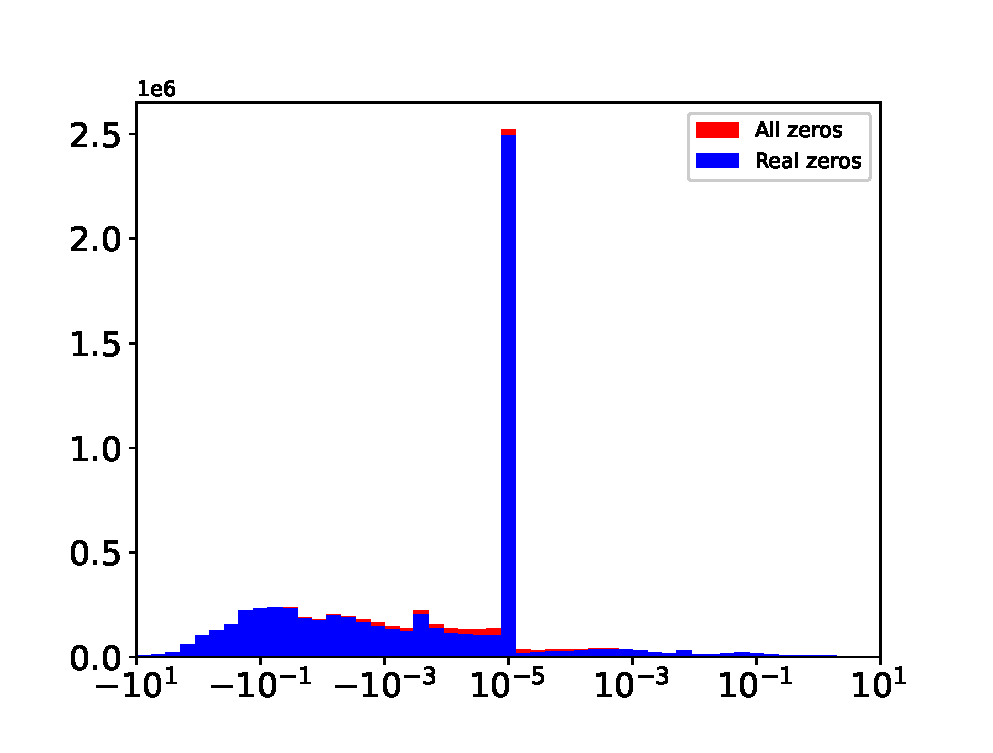
\includegraphics[height=3.2in]{complex_vertint_cutoff.eps}
  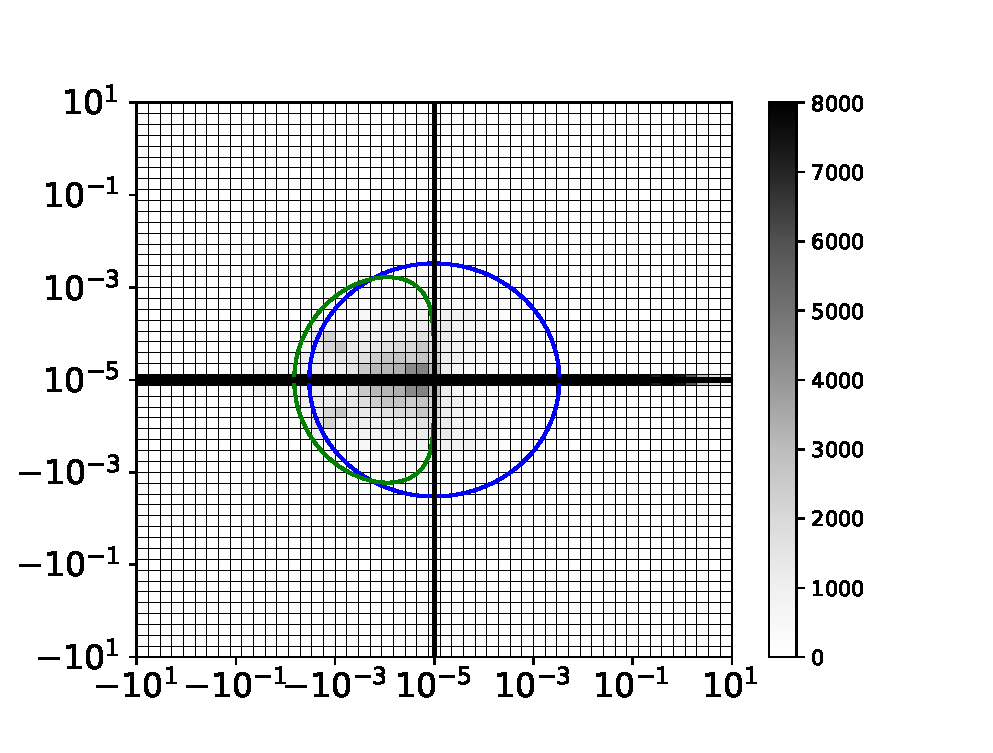
\includegraphics[height=3.2in]{complex_eigenvalues.eps}
  \end{center}
  \caption[Graphs of complex eigenvalues of the Jacobian of MG2]{Graphs of complex eigenvalues of the Jacobian of MG2, using a log scale. Eigenvalues with magnitude less than \SI{e-5}{\second} are placed at the origin. Top panel: A histogram comparing real zeros (taken to be those with $\le \SI{e-5}{\second^{-1}}$ imaginary part) with the real parts of all zeros, showing that almost all eigenvalues are real (for more detail see Figures \ref{neg-eig-hist}-\ref{pos-eig-hist}). Bottom panel: Distribution of eigenvalues in the complex plane, with a circle at $(\SI{300}{\second})^{-1}$ for comparison (blue), as well as the region of absolute stability for the Euler method (green). Eigenvalues near the real axis exceed the maximum of the color scale in this plot.}
  \label{complex-eigs}
\end{figure}

\subsection{Results}

\label{sec:timescales-results}

Figures \ref{neg-eig-hist} and \ref{pos-eig-hist} contain histograms of MG2's eigenvalues for grid cells above the \SI{e-7}{\gram\per\kilo\gram\per\second} cutoff for total water mass difference. These eigenvalues are further categorized based on whether they are associated with active or inactive processes, where an active process is one that either affects water mass above a rate of \SI{e-7}{\gram\per\kilo\gram\per\second}, or affects a hydrometeor number above a rate of \SI{2.98e-3}{\per\kilo\gram\per\second}, which is equivalent to the rate of \SI{400}{\micro\meter} diameter rain particles that would have to be introduced to produce a mass change of \SI{e-7}{\gram\per\kilo\gram\per\second}. The details of how eigenvalues are associated with processes are explained in section \ref{sec:MG2-proc-timescales}; we use association here just to indicate which eigenvalues are physically meaningful and which are akin to numerical noise. We can roughly divide these eigenvalues into five categories:

\begin{enumerate}
\item Eigenvalues associated with inactive processes (shown in blue). These eigenvalues are typically related to physics that is not active in a given regime, e.g. ice physics in a warm grid cell, so they are not as relevant to the numerics in practice.
\item Negative eigenvalues of magnitude greater than $(\SI{300}{\second})^{-1}$. These eigenvalues correspond to short-timescale processes, which have rates that may decay too rapidly for the default MG2 timescale to handle.
\item Negative eigenvalues of magnitude less than $(\SI{300}{\second})^{-1}$. These eigenvalues correspond to processes which MG2 is able to resolve, assuming roughly linear behavior of MG2.
\item Near-zero eigenvalues. These eigenvalues correspond either to extremely slow feedbacks within MG2, or to forbidden directions of motion in the phase space (particularly eigenvectors that are not tangent to surfaces of constant energy or mass, since MG2's process rates must be tangent to such surfaces).
\item Positive eigenvalues. These eigenvalues correspond to eigenvalues of processes that are temporarily in a state of positive feedback (e.g. accretion produces larger raindrops, and those larger raindrops will be effective at accreting even more cloud water). Generally speaking, MG2 avoids instability from these processes due to its nonlinearity, since all MG2 processes ``use up'' some form of mass or number, and therefore will eventually slow down over time.
\end{enumerate}

\begin{figure}[!htbp]
  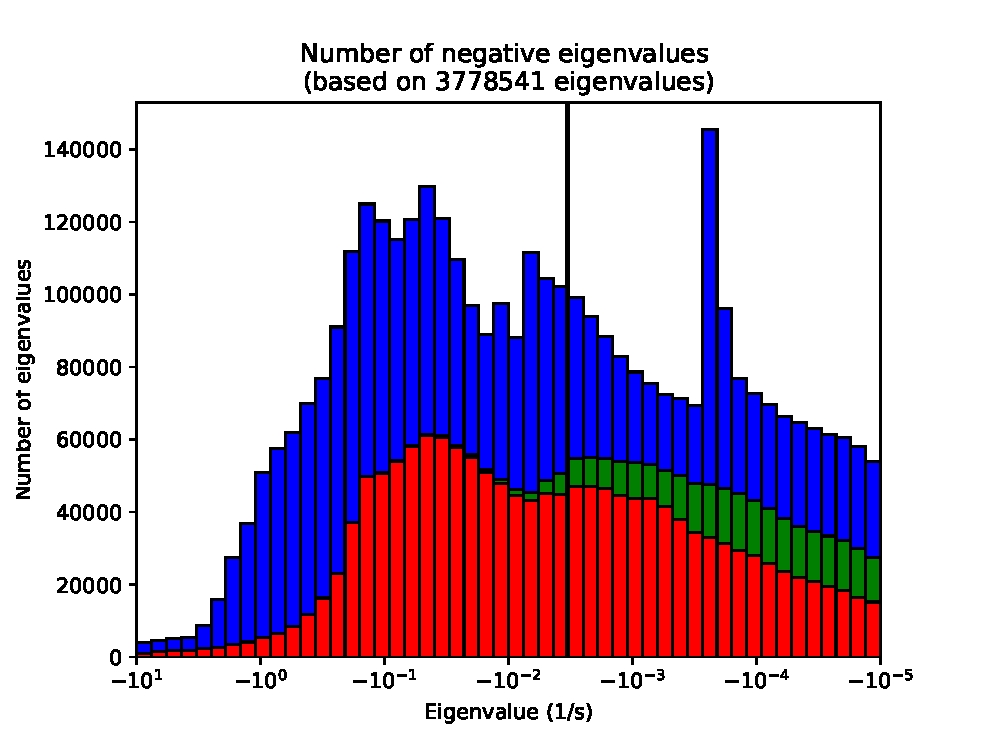
\includegraphics[width=6.5in]{./time_hist_all_values_neg.eps}
  \caption[Histogram of the negative eigenvalues of the Jacobian of MG2]{Histogram of the real parts of the eigenvalues of MG2's Jacobian, focusing on negative eigenvalues. Red bars represent eigenvalues associated primarily with an active process (see section \ref{sec:MG2-proc-timescales} for further details on this association). Green bars represent eigenvalues associated with at least one active process, but no ``primary'' process. Blue bars represent eigenvalues associated with inactive processes. A black line is placed at $(\SI{300}{\second})^{-1}$ for comparison with the MG2 time step.}
  \label{neg-eig-hist}
\end{figure}

\begin{figure}[htbp]
  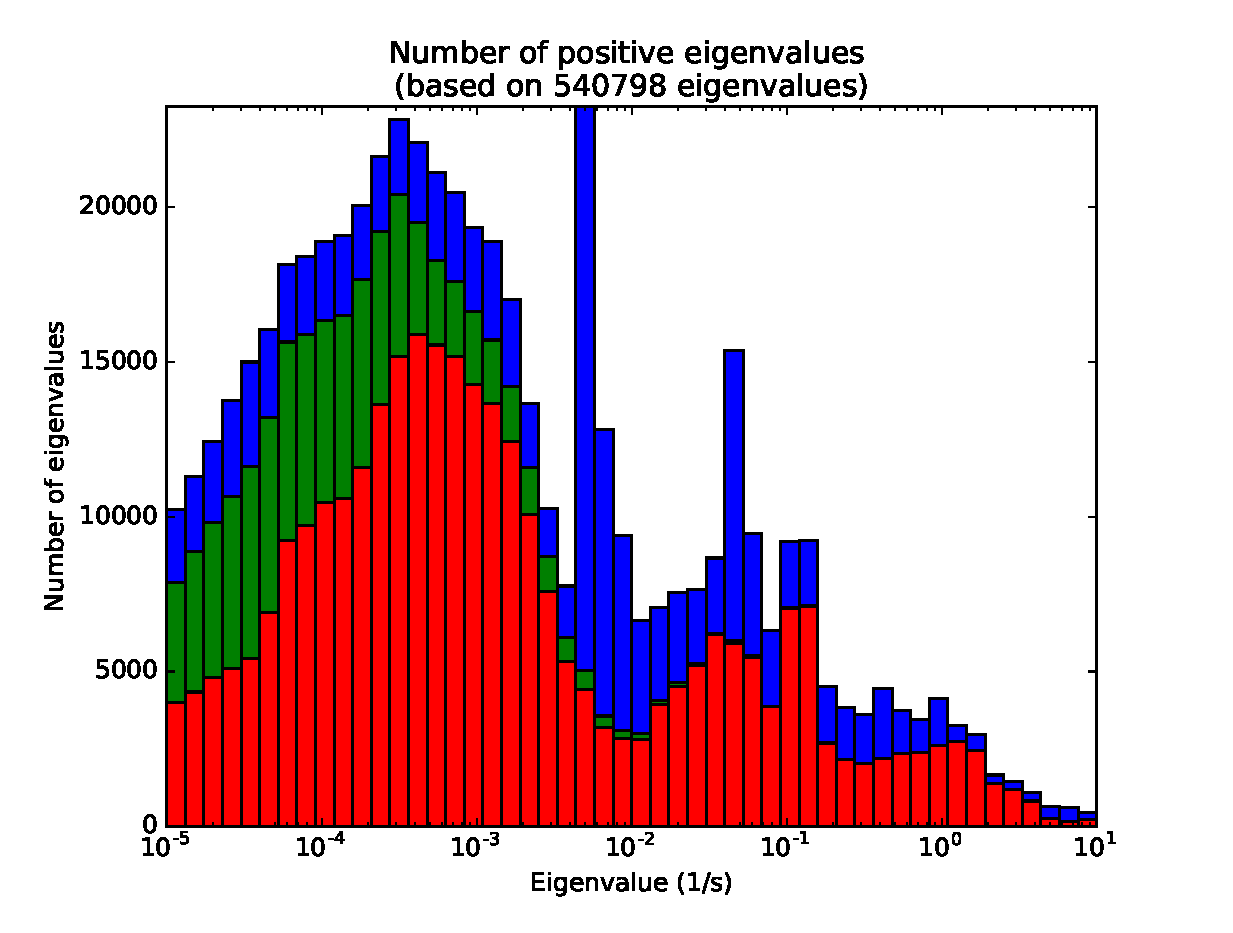
\includegraphics[width=6.5in]{./time_hist_all_values_pos.eps}
  \caption[Histogram of the positive eigenvalues of the Jacobian of MG2]{Histogram of the real parts of the eigenvalues of MG2's Jacobian, focusing on positive eigenvalues. Red bars represent eigenvalues associated primarily with an active process (see section \ref{sec:MG2-proc-timescales} for further details on this association). Green bars represent eigenvalues associated with at least one active process, but no ``primary'' process. Blue bars represent eigenvalues associated with inactive processes.}
  \label{pos-eig-hist}
\end{figure}

In general we were most interested in dealing with the second case, the large negative eigenvalues, since these are common and correspond to cases where MG2's large timescale is likely to cause problems. Note that while the forward Euler method is absolutely stable up to eigenvalues of $(\SI{150}{\second})^{-1}$ at this time step, the $(\SI{300}{\second})^{-1}$ threshold is the point at which the method will produce a monotonic decay in the error. This is more relevant for avoiding negative mass concentrations, and therefore for avoiding triggering limiters that artificially constrain the process rates. Figure \ref{neg-eig-hist} shows that there are a great number of timescales that are not adequately resolved at MG's current time step (by this measure, even more than the number that do seem adequately resolved).

We also wanted to understand the nature of the positive eigenvalues, since these eigenvalues are always outside the region of stability for the forward Euler method (though this may not be as bad as it seems, as we discuss in section \ref{sec:proc-assoc-results}).

In order to better interpret this result, however, we needed to associate the eigenvalues more closely with both specific sets of processes within MG2, and the physical conditions under which these eigenvalues arise. For instance, there may be cases where the model is formally unstable without limiters at a given time step, but in practice there is little difference between the resolved and limited behaviors.

\section{Connecting Timescales to Specific Processes} \label{sec:MG2-proc-timescales}

Documenting the timescales of MG2 processes was of inherent interest, but we were particularly interested in the finding that MG2 is often integrated using a $\Delta t$ which is too large to represent the processes it represents. Substepping all of MG2 in order to capture these timescales is not computationally feasible, but numerically accurate solutions may still be affordable if the need for substepping could be isolated to just a few processes.

\subsection{Methodology}
\subsubsection{Measuring Eigenvalue-to-Process Associations}

We sought to assign each eigenvalue from Sect. \ref{sec:MG2-timescales} to one or more of the MG2 processes listed in Table \ref{tab:processes}. Let us label the grid-cell output tendencies from applying MG2 to state $\mathbf{s}$ as $\mathbf{r} = \partial \mathbf{s}/\partial t$. The Jacobian $J_{\mathbf{r}}$ has $i,j$th entry $\partial r_i/\partial s_j$ where $r_i$ is the ith entry in $\mathbf{r}$ and $s_j$ is the $j$th entry in $\mathbf{s}$. As noted above, $J_{\mathbf{r}}$ is diagonalizable for the states that were of interest for us, so matrices of eigenvalues $\Lambda$ and eigenvectors $V$ exist such that $V \Lambda V^{-1} = J_{\mathbf{r}}$.

If we label the tendencies due to a particular process $p$ as $\mathbf{r}_p$, then $\Sigma_{p=1}^{P}\mathbf{r}_p = \mathbf{r}$. This leads directly to the identity
%-------------------------------------
\begin{eqnarray}
  \Lambda = V^{-1} (J_{\mathbf{r}}) V &= \Sigma_{p=1}^{P}V^{-1} (J_{\mathbf{r}_p}) V
\end{eqnarray}
%-------------------------------------
which is the heart of our association method. Now construct a matrix $\tilde{C}$ of dimensions $N$ (number of eigenvalues) by $P$ (number of processes to consider) whose $n,p$th entry $\tilde{C}_{np}$ is the $n$-th diagonal element of $V^{-1} (J_{\mathbf{r_p}})V$. Since it depends only on these diagonal elements, $\tilde{C}$ is independent of the scaling of the columns of $V$. Additionally,
%------------------------------------
\begin{eqnarray}
  \Sigma_{p=1}^{P}\tilde{C}_{np} &= \lambda_{n}
\end{eqnarray}
%-------------------------------------
so the $n$th row of $\tilde{C}$ represents the contributions from each process to the value of $\lambda_{n}$. The elements that contribute to a particular eigenvalue may be of different signs. Two large-magnitude values of $\tilde{C}_{np}$ may add to produce a larger $\lambda_{n}$, or they may partially cancel to produce a smaller $\lambda_{n}$. In either case, however, we would say that the largest magnitude values in $\tilde{C}$ have the most influence on the corresponding eigenvalues.

As a final step, normalize $\tilde{C}$ by taking the absolute value of each element, and by dividing each row by its $1$-norm, producing a new matrix $C$. Then each element of $C$ describes the fractional contribution of its column's process to its row's eigenvalue. If any element of $C$ is greater than \num{0.5} (our heuristic for whether at least \SI{50}{\percent} of an eigenvalue's magnitude can be attributed to a particular process), then we say that the eigenvalue for that row is \emph{primarily associated} with the process for that column. This is how the colors in Figures \ref{neg-eig-hist}-\ref{pos-eig-hist} are derived: the red bars count eigenvalues primarily associated with active processes, blue bars correspond to inactive processes, and green bars represent eigenvalues without a primary association. We are mainly concerned with large-magnitude eigenvalues, which almost all have a primary association with a particular process.

For purposes of this study, we treated the effects of MG2's size limiters as if they were a separate physical process. This was largely because MG2's state can become unrealistic or invalid if these limiters are disabled, so we were not able to disable them as we had with other instantaneous processes, and it was therefore necessary to account for their effects on MG2's state. Note also that these limiters are not applied purely for artificial, numerical reasons, since the maximum size limiters are also the means by which MG2 accounts for the spontaneous breakup of large particles, which is important especially for a reasonable treatment of precipitation.

\subsubsection{Correlation of Multiple Processes}

In addition to identifying processes associated with particular timescales, we wanted to identify tightly coupled processes. Such processes must be solved simultaneously or substepped together in order to obtain numerically accurate solutions. In addition, accounting for such coupling is needed in order to create useful conceptual models of microphysical behavior.

We hypothesized that processes that are tightly coupled in this way would be tend to be associated with the same eigenvalues. That is, while most eigenvalues have a single \emph{primary} association with another process, there are also large values of $C$ linking these eigenvalues to other processes, and we believed that this might signify cases where both processes must be solved together for accurate time integration.

To identify such possible sets of tightly coupled processes, we therefore first tallied the number of eigenvalues with primary associations to each process. We then looked at the average value of $C$ across all eigenvalues primarily associated with a given process. If, for instance, eigenvalues that are primarily associated with autoconversion also typically have strong association with accretion, then we would focus on autoconversion/accretion coupling for further study and optimization.

\subsection{Results}
\label{sec:proc-assoc-results}

We will first examine the association between positive eigenvalues and specific processes, shown in Figure \ref{process-2D-pos-eig}.

\begin{figure}[htbp]
  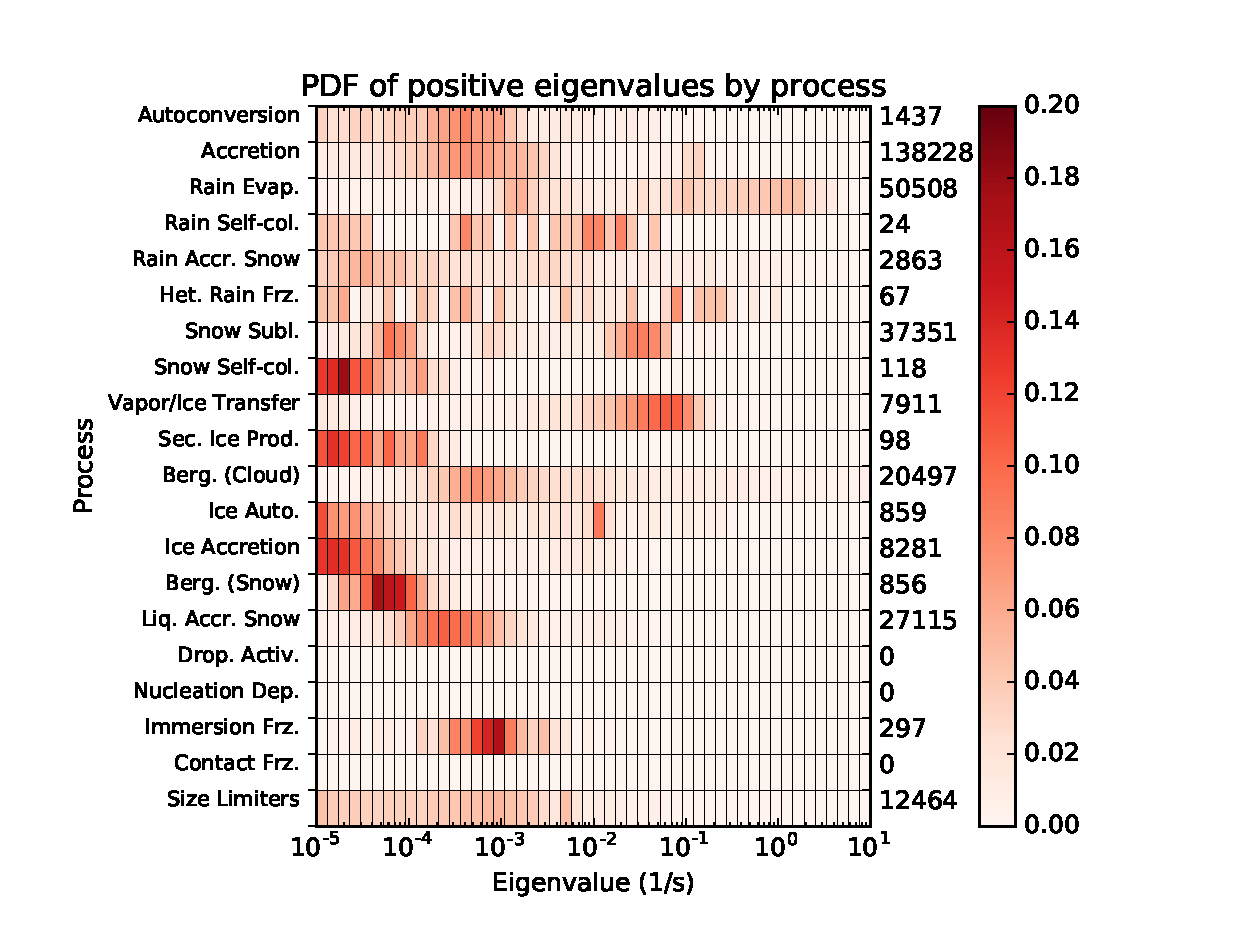
\includegraphics[width=6.5in]{./time_hist_process_2D_pos.eps}
  \caption[PDF of positive eigenvalues of the Jacobian of MG2, separated by process]{PDF of positive MG2 Jacobian eigenvalues, based on process primarily associated with each eigenvalue. Each row sums to \num{1}, except for processes with no associated positive eigenvalues. The right-hand y-axis label shows the number of positive eigenvalues associated with each process.}
  \label{process-2D-pos-eig}
\end{figure}

Many positive eigenvalues that are associated mainly with accretion-related processes (e.g. note the large number of eigenvalues associated with liquid accumulation onto rain and snow in Figure \ref{process-2D-pos-eig}). These eigenvalues are positive when the accumulating particles are small and few in number, since in this case the initial accretion increases the size of the particles, making them better at accumulating additional mass. In the long run, this is not a threat to the stability of the model, since eventually the accretion will begin to deplete the cloud, which will cause the rate of accretion to slow.

\begin{figure}[htbp]
  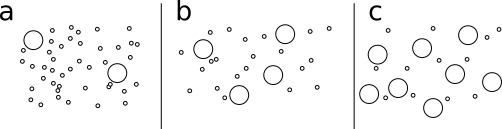
\includegraphics[width=6.5in]{./accretion_regimes.png}
  \caption[Diagram of accretion regimes]{Diagram of accretion regimes, with large circles representing rain drops and small circles representing cloud droplets. In case (a), the cloud mass is still much larger than the rain mass. As the rain accretes more liquid mass, it becomes more effective at accreting additional mass, so accretion experiences positive feedback. In case (c), the rain has already accreted most of the cloud, and further depletion of cloud mass slows the accretion rate, producing negative feedback. In case (b), cloud and rain mass are comparable, and these effects are in balance, producing only weak positive or negative feedback.}
  \label{accretion-regimes}
\end{figure}

As a concrete example, consider the accretion of cloud liquid onto rain, which responds to different conditions as shown in Figure \ref{accretion-regimes}. If we take this to be the only process active in a grid cell, MG2 gives us the following differential equation, where $c_a$ (the accretion enhancement factor) is typically a constant:

\begin{align}
  \frac{\partial}{\partial t}
  \begin{pmatrix}
    q_c \\ n_c \\ q_r
  \end{pmatrix}
  = 67 c_a
  \begin{pmatrix}
    -(q_c q_r)^{1.15} \\ q_c^{0.15} q_r^{1.15} n_c \\ (q_c q_r)^{1.15}
  \end{pmatrix}
\end{align}

The eigenvalues and eigenvectors of the Jacobian in this case are:

\begin{align}
  \lambda_1 &= 67 (1.15) c_a (q_c - q_r) (q_c q_r)^{0.15} & \lambda_2 &= -67 c_a q_c^{0.15} q_r^{1.15} & \lambda_3 &= 0 \\
  \mathbf{v}_1 &= 
  \begin{pmatrix}
    -q_c \\ -n_c \\ q_c
  \end{pmatrix} & \mathbf{v}_2 &= 
  \begin{pmatrix}
    0 \\ 1 \\ 0
  \end{pmatrix} & \mathbf{v}_3 &= 
  \begin{pmatrix}
    -q_c \\ -n_c \\ q_r
  \end{pmatrix}
\end{align}

The trajectory of the system always points in the direction of the first eigenvector, and therefore this eigenvector describes the response to errors in accretion rate. This the only one of the three that can be positive. The second of these eigenvalues governs errors in cloud droplet number, and is always negative when accretion is active. The third eigenvalue governs the response to errors that do not change the accretion rate but violate conservation of mass (except in the degenerate case where $q_c = q_r$), and is always \num{0}.\footnote{We stated above that the Jacobian of MG2 is \emph{almost} never defective when hydrometeors are present. This simplified system shows one of the rare exceptions: the Jacobian is defective when $q_c = q_r$. This is not much of a problem for our analysis, since the accretion rate is at its highest when $q_c \approx q_r$, so the trajectory spends very little time in the neighborhood of this point, and since our focus is on larger magnitude eigenvalues in any case.}

For a given initial condition, we can define $q_{tot} = q_c + q_r$, and then convert to a nondimensionalized time $t'$ using the transformation $t' = 67 c_a q_{tot}^{1.3} t$. The time evolution of the nondimensionalized system, including the evolution of two eigenvalues, is shown in Figure \ref{accretion-trajectory}. While $\lambda_1$ is initially positive, it changes sign once $q_c$ is sufficiently depleted, which is typical of accretion processes. The main threat to the stability of the system occurs when $q_c < 0$ (triggering the conservation limiters). For the forward Euler method, this occurs when $\lambda_2 \Delta t < -1$, which in turn is most likely to occur when $q_c < q_r$ and both nonzero eigenvalues are strongly negative.

Although the system will typically remain stable when $\lambda_1$ is positive, the error from the forward Euler method will still have some effect. Using a coarse time step will cause the accretion rate to grow more slowly, delaying the onset of peak accretion by $\sim$\num{1.8} timesteps (see Figure \ref{accretion-time}). We believe this delay is not important for MG2, however, because when $q_c \gg q_r$, autoconversion, not accretion, dominates rain production.

\begin{figure}[htbp]
\begin{center}
  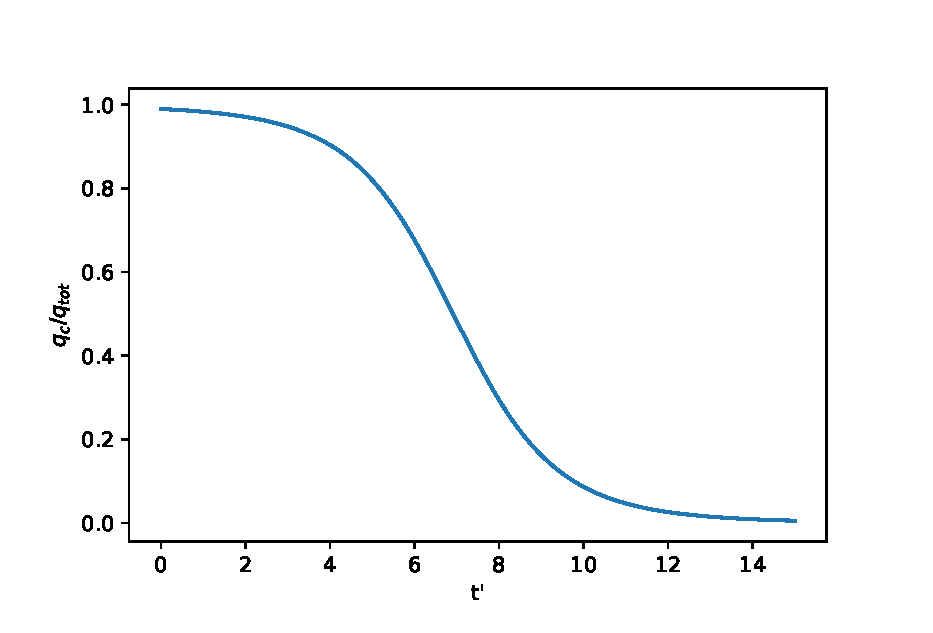
\includegraphics[height=3.5in]{./accretion_qc.eps}
  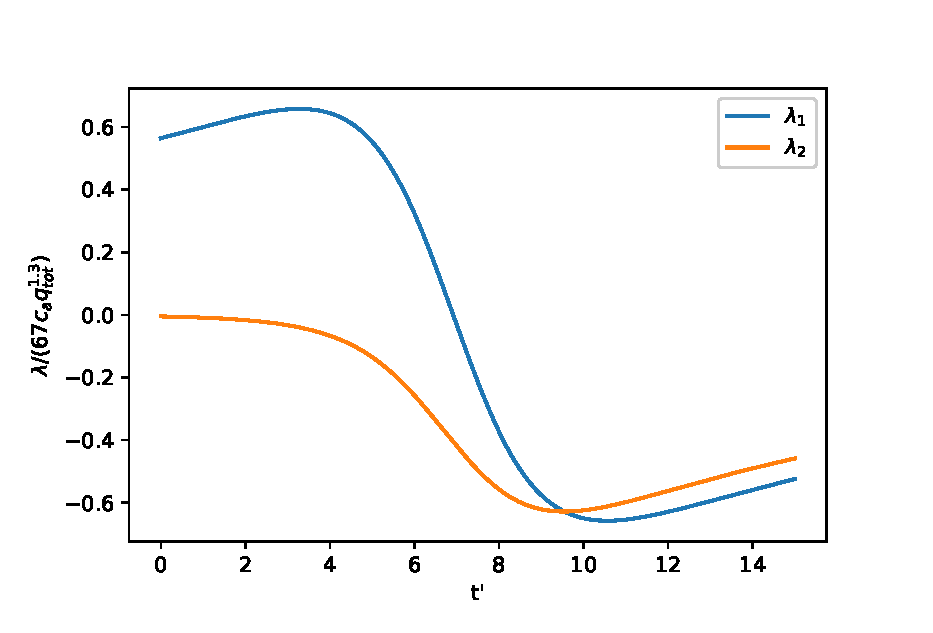
\includegraphics[height=3.5in]{./accretion_lambdas.eps}
\end{center}
  \caption[Trajectories of accretion subsystem]{The values of $q_c$ (top) and two eigenvalues (bottom) over time for a grid cell where only MG2's accretion is active.}
  \label{accretion-trajectory}
\end{figure}

\begin{figure}[htbp]
  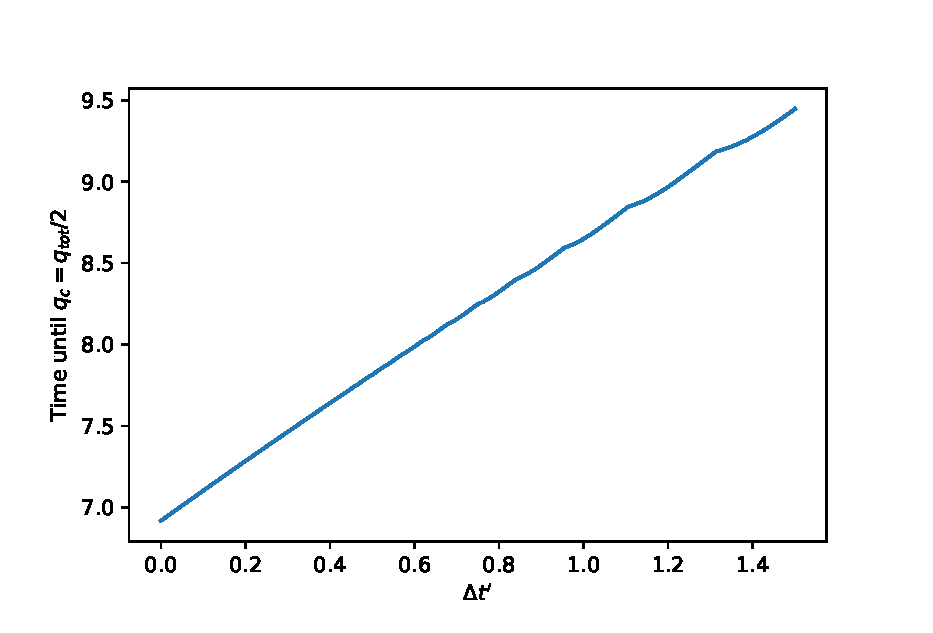
\includegraphics[width=6.5in]{./accretion_half_time.eps}
  \caption[Time to accrete half of a cloud's mass]{Time taken to accrete half a cloud's mass versus time step used for simulations using the forward Euler method, using linear interpolation between time steps to determine when $q_c=q_{tot}/2$. All simulations start from an initial condition where 1\% of total mass is rain. Slope of this curve for small time steps is approximately \num{1.86}, decreasing slightly as time step size increases.}
  \label{accretion-time}
\end{figure}

Setting aside positive eigenvalues from accretion, most other positive eigenvalues of MG2 are primarily associated with evaporation or sublimation. (Again in Figure \ref{process-2D-pos-eig}, there are large counts for rain evaporation, snow sublimation, and the Bergeron process.) These eigenvalues are positive mainly when the affected particles are small and few in number, as such particles rapidly evaporate when out-of-cloud. In such cases, the particle mass rapidly drops to zero, and the temporal resolution should not be relevant to the final state of the system.

Turning back to the negative eigenvalues, we wanted to examine the processes associated with the smallest timescales. As seen in Figure \ref{process-2D-neg-eig}, these processes are:

\begin{enumerate}
\item Accretion of cloud water by rain.
\item Rain evaporation.
\item Rain self-collection.
\item Snow sublimation.
\item Snow self-collection.
\item Vapor/Ice transfer.
\end{enumerate}

Other processes that were active with relatively short timescales include the Bergeron process and heterogeneous rain freezing, but we believe that the process rates are not being accurately calculated by our driver, and so we are less concerned about the apparent short timescales involved. The Bergeron process rate calculation is believed to be one of the least accurate parameterizations in MG2, primarily because it is poorly suited to the coarse spatial resolution used for GCMs, sometimes even resulting in a rate that is orders of magnitude too large \parencite{Tan2016,Zhang2019}. Reducing the time integration error is simply not a priority until this issue is addressed. As for the heterogeneous rain freezing, it is the process least likely to behave the same way in our driver as it does in E3SMv1, because we have disabled instantaneous freezing of rain, and the heterogeneous process should be expected to be more active to compensate.

The particular processes that we examined in more detail were rain evaporation, self-collection, and accretion of cloud water.  Partially this was because the purely liquid processes were easier to examine in isolation from the other physics, and partly this was because in practice the vapor/ice transfer was usually associated with small timescales only when the effect of this process was small anyway, so the error due to finite time resolution was small. In particular, sublimation of a small ice mass in relatively dry air can be quite rapid, but leads to the same behavior as given by the limited behavior, namely that the ice sublimates completely and rapidly.

We can also note that almost no eigenvalues are associated with the external processes, which is what we expect since these process' rates don't directly depend on the MG2 inputs, and only interact with MG2's physics due to being affected by the conservation limiters. In our data set, we found only three eigenvalues associated with contact freezing, a few thousand associated with immersion freezing, and none with nucleation deposition or droplet activation.

\begin{figure}[htbp]
  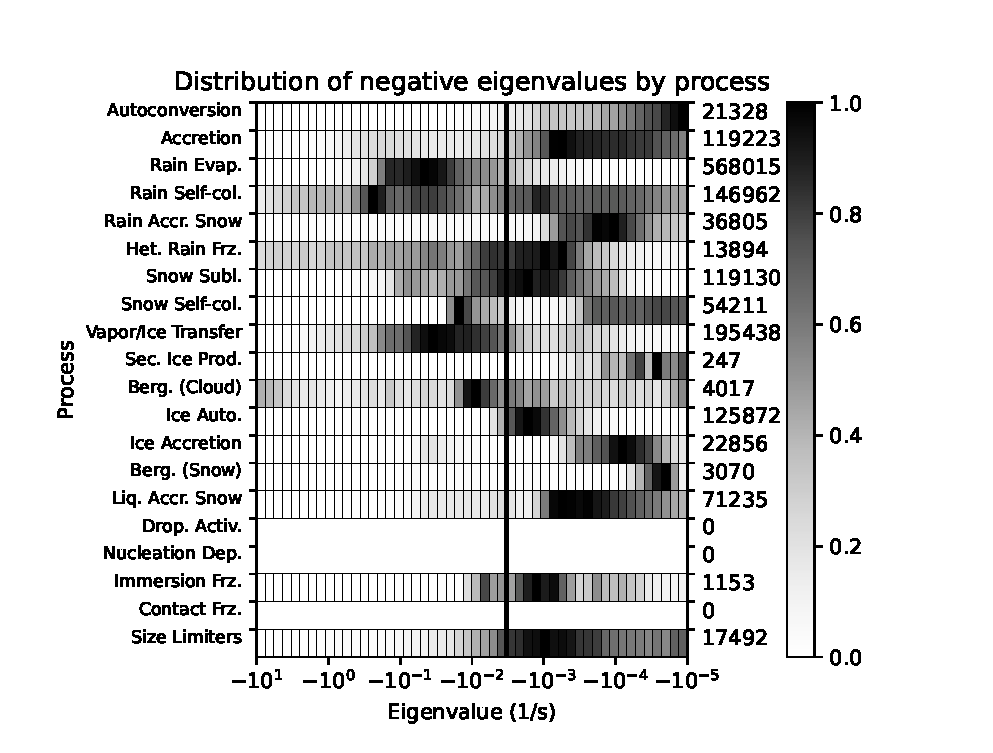
\includegraphics[width=6.5in]{./time_hist_process_2D_neg.eps}
  \caption[PDF of negative eigenvalues of the Jacobian of MG2, separated by process]{PDF of negative MG2 Jacobian eigenvalues, based on process primarily associated with each eigenvalue. Each row sums to \num{1}, except for processes with no associated negative eigenvalues.The right-hand y-axis label shows the number of negative eigenvalues associated with each process. A black line is placed at $(\SI{300}{\second})^{-1}$ for comparison with the MG2 time step.}
  \label{process-2D-neg-eig}
\end{figure}

Figure \ref{process-association} shows the degree to which different processes were associated with the same eigenvalues (and hence timescales). Looking at timescales associated primarily with the processes listed above, we found the following:

\begin{enumerate}
\item Accretion of cloud water by rain is associated with autoconversion.
\item Rain self-collection is strongly associated with rain evaporation.
\item The degree of association between ice processes is quite complex. In particular, vapor/ice transfer is associated with several processes, possibly because it is mildly active in a very large number of grid cells.
\end{enumerate}

\begin{figure}[htbp]
  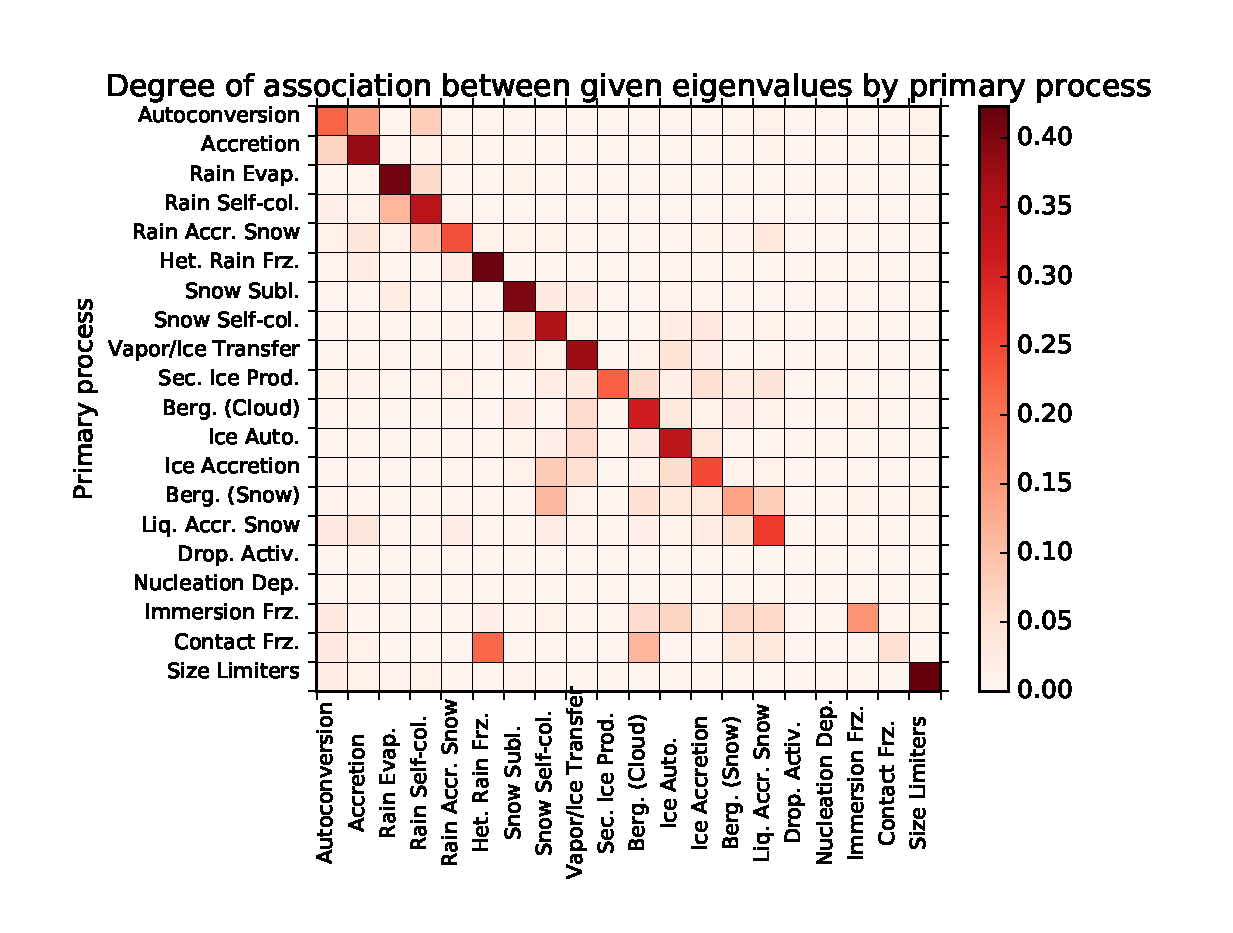
\includegraphics[width=6.5in]{./process_association.eps}
  \caption[Association between pairs of processes in MG2 based on Jacobian eigenvalues]{Association between pairs of processes in MG2. Each row shows the average association index ($C$) for eigenvalues associated with a given primary process. That is, each row of the table shows the average value of a row of $C$ for eigenvalues primarily associated with the process shown on the left axis. By our definition of primary association, this means that all elements on the diagonal have values of at least \num{0.5}, so each entry on the diagonal has had its value reduced by \num{0.5} to fit in the same color range.}
  \label{process-association}
\end{figure}

As Figure \ref{process-2D-neg-eig} shows, the timescales associated with both liquid and ice autoconversion were relatively long. We therefore expected that the regime in which, say, liquid autoconversion and accretion interact most heavily would be different from the regime in which accretion by rain is associated with short timescales, and therefore we hypothesized that autoconversion should not require a short time step to adequately resolve, despite its association with accretion.

On the other hand, rain self-collection and evaporation were both primarily associated with the same short timescales, and so it appeared less likely that we could resolve rain-related processes without using a relatively short timescale for both.

\section{Decomposition by Weather Regime} \label{sec:MG2-regime}

Microphysics operates differently in different meteorological conditions. In particular, only a few microphysical processes are typically active at any particular point in space and time. Thus breaking cases down by weather regime can simplify the task of understanding model behavior. Such decomposition is also important because processes are likely to have different timescales depending on the weather regime they're in. For instance, the rate of accretion is fairly steady when rain and cloud mass are similar, but the accretion rate decreases rapidly when cloud becomes depleted, and the associated timescale is therefore much smaller in the latter case.

\subsection{Methodology}

We accomplished this decomposition by normalizing all process rates by typical values (so all processes were given approximately equal weight) and using a simple $k$-means algorithm to cluster grid cells based on process rates, so that we could treat the clusters as separate regimes.

We were interested in finding clusters containing qualitatively different, common types of behavior to examine in further detail, not in an objective categorization of all types of grid cells in the model. For this purpose we were content to use a degree of hand-tuning to determine both the total number of clusters and the scaling of process rates used in the clustering algorithm (for instance, reducing the effect of the Bergeron process). We iterated with changes to the cluster number and scaling until we found \num{10} clusters that had reasonably distinct process rates from one another.

Once this was accomplished, we could then look at the eigenvalues associated with the Jacobian for each cluster, in order to determine which regimes were likely to have short timescale behavior based on process rates alone.

\subsection{Results}

Table \ref{tab:clusters} gives a brief summary of the most active processes in each of these clusters, specifically those with mean rate above \SI{e-5}{\gram\per\kilo\gram\per\second} (or \SI{0.298}{\per\kilo\gram\per\second} for precipitation self-collection), as well as the number of grid points in each cluster. Note that these rates are \num{100} times greater than those used in section \ref{sec:timescales-results}, since we are describing those processes that dominate the physics for each cluster, rather than those that simply have some appreciable activity. Note that cluster 0, which consists of generally clear-sky grid cells where no processes are particularly active, comprises the majority of our data set.

While the Bergeron process for cloud ice and heterogeneous rain freezing may seem quite large in many clusters, these should be disregarded for two reasons. Firstly, as noted in section \ref{sec:proc-assoc-results}, these two processes are not likely to be well represented in our driver. For the Bergeron process, this is due to the low accuracy of MG2's representation of this process at the spatial resolutions used by GCMs. We believe that there will be little benefit to improving time integration of the Bergeron process until this more fundamental concern is addressed. As for the heterogeneous rain freezing, this process is likely affected by our standalone driver deviating from the behavior of MG2 within E3SMv1, in particular by the fact that the instantaneous rain freezing has been disabled. Secondly, our scaling deemphasized these processes, so they had the less impact on the clustering algorithm itself than the other MG2 processes.

\begin{table}
  \centering
  \scriptsize
  \begin{tabular}{|c|p{0.35\linewidth}|p{0.35\linewidth}|r|}
    \hline
    Index & Cluster Description & Active Processes & \# Grid Points \\
    \hline
    0 & MG2 mostly inactive. & Berg. (Cloud): \SI{1.03e-5}{\gram\per\kilo\gram\per\second} & \num{3404586} \\
    \hline
    1 & Ice cloud growth. & Berg. (Cloud): \SI{2.53e-2}{\gram\per\kilo\gram\per\second} \newline Vapor/Ice Transfer: \SI{3.58e-5}{\gram\per\kilo\gram\per\second} \newline Het. Rain Frz.: \SI{1.03e-5}{\gram\per\kilo\gram\per\second} & \num{2504} \\
    \hline
    2 & Snow accumulating rain and cloud liquid. & Het. Rain Frz.: \SI{1.11e-4}{\gram\per\kilo\gram\per\second} \newline Rain Accr. Snow: \SI{2.11e-5}{\gram\per\kilo\gram\per\second} \newline Liq. Accr. Snow: \SI{1.96e-5}{\gram\per\kilo\gram\per\second} \newline Rain Self-col.: \SI{2.57}{\per\kilo\gram\per\second} & \num{23854} \\
    \hline
    3 & Early/light rain production. & Autoconversion: \SI{1.59e-5}{\gram\per\kilo\gram\per\second} \newline Accretion: \SI{1.09e-5}{\gram\per\kilo\gram\per\second} \newline Rain Self-col.: \SI{16.16}{\per\kilo\gram\per\second} & \num{22378} \\
    \hline
    4 & Snow-producing cloud with out-of-cloud precipitation. & Het. Rain Frz.: \SI{1.26e-4}{\gram\per\kilo\gram\per\second} \newline Berg. (Cloud): \SI{1.00e-4}{\gram\per\kilo\gram\per\second} \newline Ice. Auto.: \SI{3.66e-5}{\gram\per\kilo\gram\per\second} \newline Snow Subl.: \SI{3.06e-5}{\gram\per\kilo\gram\per\second} \newline Rain Evap.: \SI{1.09e-5}{\gram\per\kilo\gram\per\second} \newline Snow Self-col.: \SI{1.40}{\per\kilo\gram\per\second} & \num{694} \\
    \hline
    5 & Out-of-cloud, mixed precipitation. & Berg. (Cloud): \SI{2.90e-4}{\gram\per\kilo\gram\per\second} \newline Rain Evap.: \SI{3.59e-5}{\gram\per\kilo\gram\per\second} \newline Snow Subl.: \SI{3.21e-5}{\gram\per\kilo\gram\per\second} \newline Rain Self-col.: \SI{0.619}{\per\kilo\gram\per\second} & \num{5456} \\
    \hline
    6 & Late/heavy rain production. & Accretion: \SI{3.80e-5}{\gram\per\kilo\gram\per\second} \newline Autoconversion: \SI{1.15e-5}{\gram\per\kilo\gram\per\second} \newline Rain Self-col.: \SI{47.46}{\per\kilo\gram\per\second} & \num{5404} \\
    \hline
    7 & Heavy rain in a concentrated area. & Rain Evap.: \SI{1.25e-4}{\gram\per\kilo\gram\per\second} \newline Rain Self-col.: \SI{511}{\per\kilo\gram\per\second} & \num{849} \\
    \hline
    8 & Snow-producing cloud with all precipitation in cloud. & Het. Rain Frz.: \SI{3.63e-4}{\gram\per\kilo\gram\per\second} \newline Berg. (Cloud): \SI{2.73e-5}{\gram\per\kilo\gram\per\second} \newline Liq. Accr. Snow: \SI{1.37e-5}{\gram\per\kilo\gram\per\second} \newline Ice. Auto.: \SI{1.00e-5}{\gram\per\kilo\gram\per\second} \newline Rain Self-col.: \SI{1.00}{\per\kilo\gram\per\second} \newline Snow Self-col.: \SI{0.535}{\per\kilo\gram\per\second} & \num{4579} \\
    \hline
    9 & Rain over a broad area. & Rain Evap.: \SI{3.48e-4}{\gram\per\kilo\gram\per\second} \newline Rain Self-col.: \SI{44.5}{\per\kilo\gram\per\second} & \num{29040} \\
    \hline
  \end{tabular}
  \caption{Description of clusters found through k-means algorithm}
  \label{tab:clusters}
\end{table}

Note that this provides another, simpler way to look at associations between processes. Looking again at liquid autoconversion and accretion, we see that these two processes are active together in clusters 3 and 6, but that the rate of accretion is much larger in cluster 6. We can then look at the eigenvalues of the Jacobian based on cluster, which is shown in Figure \ref{cluster-2D-neg-eig}. Unsurprisingly, the negative eigenvalues are much larger in cluster 6, implying that the short timescales are associated with the heavy accretion present in cells with a relatively large in-cloud rain mass.

\begin{figure}[htbp]
  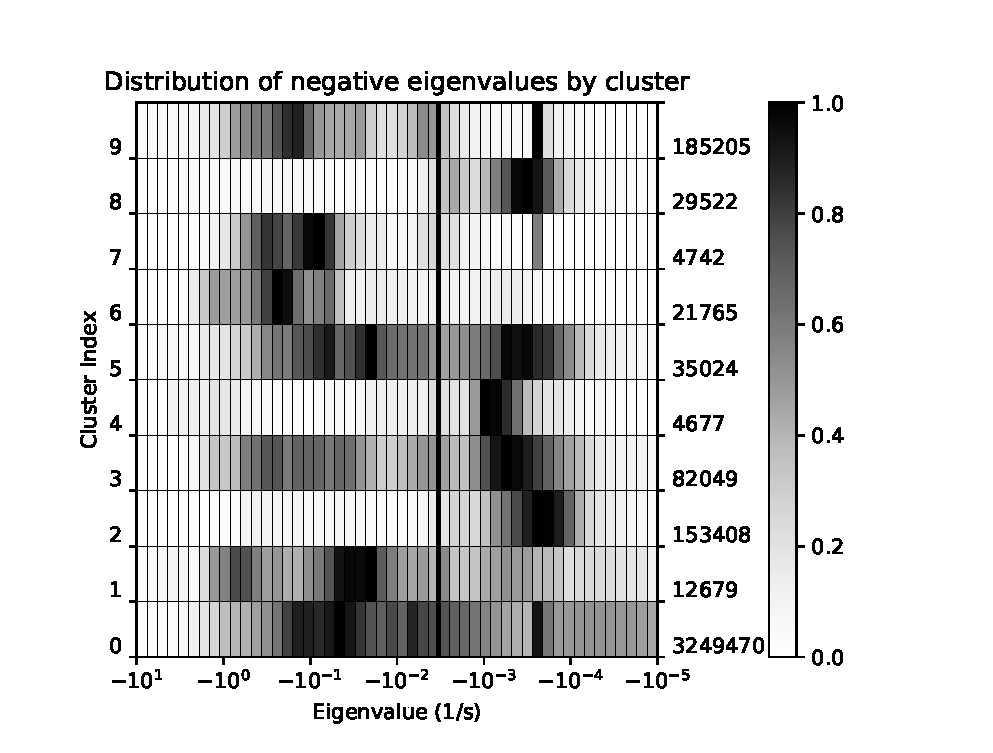
\includegraphics[width=6.5in]{./time_hist_cluster_2D_neg.eps}
  \caption[PDF of negative eigenvalues of the Jacobian of MG2, separated into clusters corresponding to different regimes]{PDF of negative MG2 Jacobian eigenvalues, based on cluster of grid cell where the eigenvalue was calculated. The right-hand y-axis label shows the number of eigenvalues plotted for grid points in each cluster.}
  \label{cluster-2D-neg-eig}
\end{figure}

Similarly, we can use other clusters to examine other sets of short timescale processes. Cluster 1 would the best test case for short timescales associated with the Bergeron process and ice deposition (if the Bergeron parameterization was made more accurate). Rain evaporation and self-collection are both active and associated with short timescales in clusters 7 and 9.

\section{Impact of Shorter Time Steps} \label{sec:MG2-impact}

In the previous sections we identified processes and combinations of processes that evolve much more rapidly than the default model step. In this section we test whether accurately resolving those processes has a big impact on model behavior.

\subsection{Methodology}

In this section, we focus on two clusters, each associated with a set of processes that we believed would change considerably if substepped so as to resolve their behavior:

\begin{enumerate}
\item Grid cells with large rain self-collection and evaporation rates, corresponding to heavy out-of-cloud rain. (Cluster 9)
\item Grid cells with large accretion rates and moderate autoconversion rates, corresponding to heavy in-cloud rain. (Cluster 6, filtered to remove grid cells with any ice process rate or rain evaporation rate above \SI{e-7}{\gram\per\kilo\gram\per\second})
\end{enumerate}

The subsampling of cluster 6 was necessary to remove cases where accretion and autoconversion were not the only active processes. This was necessary for two reasons. Firstly, the clustering algorithm alone did not perfectly separate those grid cells with only rain production from grid cells that combined rain production with evaporation/sublimation of precipitation falling from above. Secondly, in some grid cells, especially at large time step sizes, the cloud liquid is turned completely to rain. If all cloud mass is removed from a grid cell, MG2 no longer considers the fraction of the grid cell that was occupied by the cloud to be saturated, and rain evaporation turns on. Since we were interested in the effect of substepping on autoconversion and accretion specifically, we removed grid cells where this occurred from this portion of the study. It should be noted that rain self-collection is also active in cluster 6. However, autoconversion and accretion within MG2 are not functions of the rain number, so it is not necessary to account for rain self-collection to accurately represent these processes.

For each of these cases, we produced modified versions of the MG2 standalone driver from section \ref{sec:MG2-standalone}, which allowed these processes to be run at a smaller time step using the forward Euler method. For instance, for heavy in-cloud rain, autoconversion and accretion were substepped inside a nested series of loops, so that it was possible to adjust the time step of each independently of MG2 as a whole. If both processes were run at a finer time step, it was also possible to independently adjust the coupling frequency. At all levels processes were coupled using a parallel split, as in the original code. By adjusting the process time steps and coupling time steps, it was possible to determine which processes needed to be better resolved to improve MG2's accuracy, and which were less relevant.

In order to assess the accuracy of these substepped simulations, it was necessary to decide upon both a measure of error, and a ``converged'' result for comparison. To measure the error in each grid cell, we used the total water mass difference defined above ($D_w$), which for Cluster 9 was effectively identical to the evaporation rate due to the absence of other influences (recall that $D_w$ only accounts for the error in water mass, not hydrometeor number). The converged result was first approximated by using MG2 run at a very fine time step of \SI{75/512}{\second}, which is \num{1/2048} of the normal MG2 time step of \SI{300}{\second}. Using a power of two in this way is convenient for convergence studies, where the time step can be progressively halved to provide results that are closer and closer to converged.

However, this tended to underestimate the error for similarly fine time steps. The error found when using a \SI{75/512}{\second} time step for a first order method is approximately half the error found when using \SI{75/256}{\second} time step, meaning that the former is not a useful reference result for measuring the error of the latter. We therefore improved the estimate using a Richardson extrapolation. Since we are using the forward Euler method, which is a first-order method, if we denote these two results from small time steps as $\mathbf{s}_{75/512}$ and $\mathbf{s}_{75/256}$, our extrapolated reference state $\mathbf{s}_{ref}$ is simply:

\begin{align}
    \mathbf{s}_{ref} = 2 \mathbf{s}_{75/512} - \mathbf{s}_{75/256}
\end{align}

Although we expect roughly first-order convergence for these very short time steps, we do not expect to see it for much larger time steps, and in particular there is no guarantee that this will hold when the method is kept stable by limiters rather than because the method is absolutely stable at a given time step. There is little point in reducing the model time step if doing so does not much improve the accuracy, so we should hope that we can afford to use a time step short enough to reach the regime where first-order convergence holds, as a bare minimum.

\subsection{Results}

We hypothesized that for the grid cells with large rain evaporation, there would be a noticeable benefit from substepping rain self-collection as well, since our Jacobian-based analysis associates these two processes with the same short timescales.

Since these timescales are typically around \SI{20}{\second}, we also expect to see roughly first-order convergence for time steps shorter than this, but not for larger time step sizes, because for larger time steps this method (or rather, its linearization around a typical state) is not stable on this problem. The model therefore becomes increasingly dependent on limiters for longer time steps.

The actual evaporation/self-collection results are shown in Figure \ref{convergence-evap-scol}. For comparison, note that the mean evaporation rate in this cluster is about \SI{1.82e-4}{\gram\per\kilo\gram\per\second}, so the mean error at a \SI{300}{\second} time step is an appreciable fraction of the evaporation rate itself. Substepping evaporation by itself is indeed much less effective than substepping both processes together. The self-collection of raindrops is a very fast process in MG2, and accounting for this considerably reduces the rate of evaporation. In particular, for grid points in cluster 9, the self-collection causes rain drops to reach the maximum allowed size in less than \SI{300}{\second}, meaning that unless processes like rain evaporation are coupled at a smaller timescale, the particle size is effectively determined by the size limiter, not the details of the self-collection itself. This is one reason it is unsurprising that we see sub-linear convergence at larger time step sizes.

\begin{figure}[htbp]
  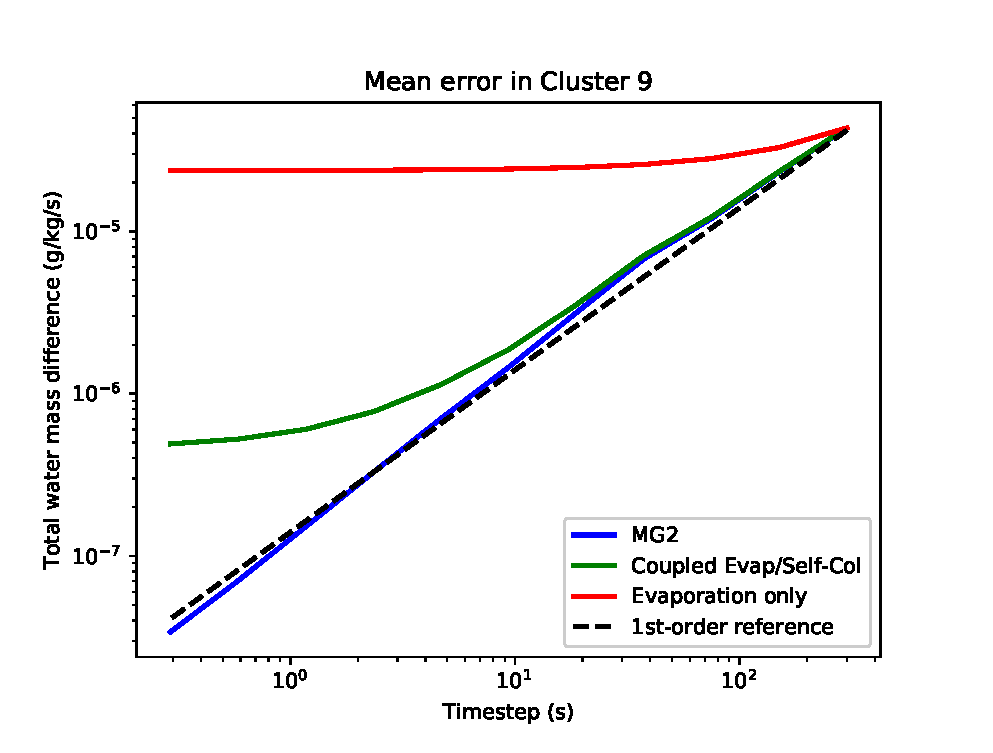
\includegraphics[width=6.5in]{./substep_convergence_mean_c9_richext.eps}
  \caption[Convergence plot for mean MG2 error in a cluster of rainy, cloudless grid cells using different substepping strategies]{Convergence plot for mean error in cluster 9 grid cells under different substepping strategies for rain evaporation and self-collection. Runs substepping all of MG2 are shown in blue. Runs substepping evaporation and self-collection together, with total MG2 time step held fixed at \SI{300}{\second}, are shown in green. Substepping evaporation alone, with all other processes at \SI{300}{\second}, shown in red. The dotted reference line has slope \num{1}.}
  \label{convergence-evap-scol}
\end{figure}

Furthermore, the rate of convergence of the model becomes first-order below a time step size of roughly \SIrange{30}{60}{\second}, both when all of MG2 is substepped and when only these two processes are substepped together. In fact, it appears faster than first-order when all of MG2 is substepped. This may be due to the fact that our ``resolved'' result is the \SI{75/512}{\second} result, and this causes some underestimation of the error in the leftmost few points on the graph. At very short time steps, the error levels off when substepping only evaporation and self-collection due to small contributions from other, non-substepped processes in the grid cell (e.g. small amounts of cloud are present, causing some accretion, though the average accretion rate in this cluster is orders of magnitude less than the evaporation rate).

For grid cells dominated by accretion and autoconversion, we expected the effect of substepping accretion to matter much more than that of autoconversion, since autoconversion is associated almost exclusively with timescales longer than the maximum MG2 step size of \SI{300}{\second}. Similar to the evaporation case, we expected that first-order convergence would occur only for timescales shorter than about \SI{5}{\second}.

Figure \ref{convergence-accr-auto} shows the results of this substepping of accretion and autoconversion in cluster 6. Accretion rates are \SI{1.13e-4}{\gram\per\kilo\gram\per\second}, so the error is again comparable to the accretion rate itself. Substepping autoconversion alone is ineffective for reducing the error. Substepping the accretion, however, can cut the errors by more than an order of magnitude, while substepping autoconversion as well improves the error by only another factor of \num{2}.

\begin{figure}[htbp]
  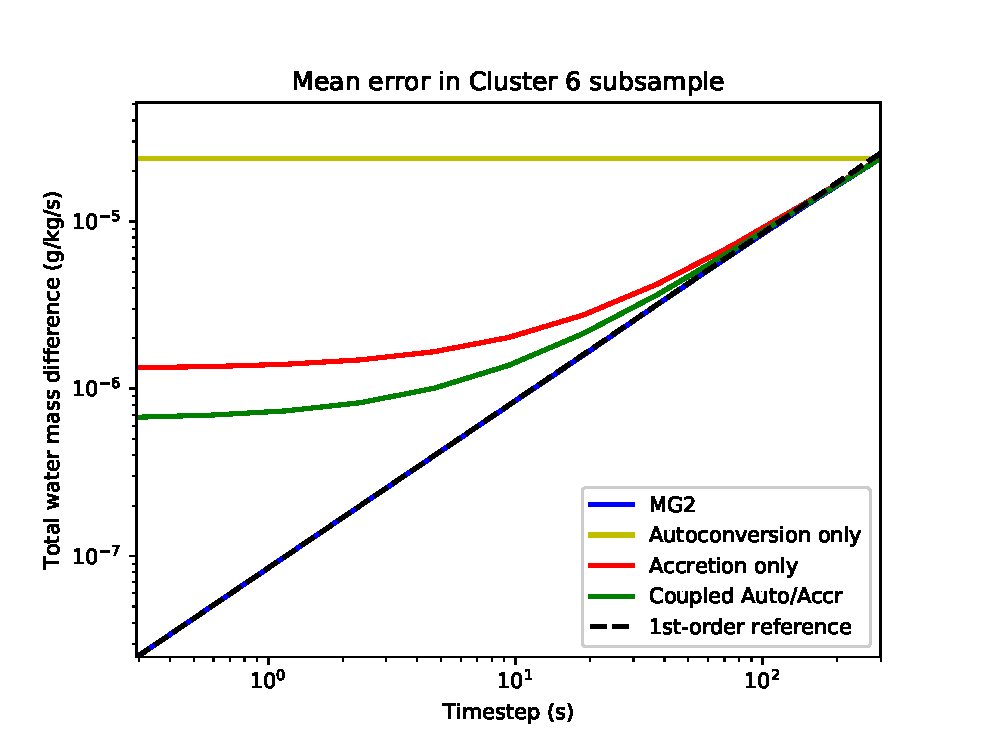
\includegraphics[width=6.5in]{./substep_convergence_mean_c6_richext.eps}
  \caption[Convergence plot for mean MG2 error in a cluster of rain-producing grid cells using different substepping strategies]{Convergence plot for mean error in cluster 6 subsample under different substepping strategies for accretion and autoconversion. Runs substepping all of MG2 are shown in blue. Runs substepping accretion and autoconversion together, with total MG2 time step held fixed at \SI{300}{\second}, are shown in green. Substepping accretion alone is shown in red, and substepping autoconversion alone is shown in yellow. The dotted reference line has slope \num{1}.}
  \label{convergence-accr-auto}
\end{figure}

However, we find, somewhat surprisingly, a near-perfect first-order convergence when substepping these processes, even out to \SI{300}{\second}. Note, again, the much smaller timescales in cluster 6 shown in Figure \ref{cluster-2D-neg-eig}, which would seem to suggest that this time step would produce instability, not linear convergence.

We came to suspect that by subsampling cluster 6, we had removed the grid points with the shortest timescales. There are three possible reasons this could happen. Firstly, the grid points with active ice processes could have been the grid points disproportionately associated with the shortest associated timescales. Secondly, the grid points with no ice processes but some evaporation at the beginning of the time step could be responsible, since some grid cells with out-of-cloud precipitation were included. Finally, some grid points could have no rain evaporation at the beginning of the time step, but develop rain evaporation over the course of a time step. In these grid points, at the beginning of the time step, all rain is considered to be inside the cloud, and no evaporation occurs. However, if the cloud is depleted to a concentration of less than \SI{e-3}{\gram\per\kilo\gram}, MG2 ignores the cloud area and assumes that all precipitation is outside the cloud, and therefore can evaporate.

Figure \ref{eig-c6-subsample} shows the results of our investigation. We find that our subsample did in fact include mostly points associated with long timescales, and excluded the majority of shorter timescales. Furthermore, the majority of points in cluster 6, especially those associated with short timescales, were points that started with no active evaporation or ice processes, but which ended up depleting enough cloud to cause MG2's evaporation process to switch on.

\begin{figure}[htbp]
  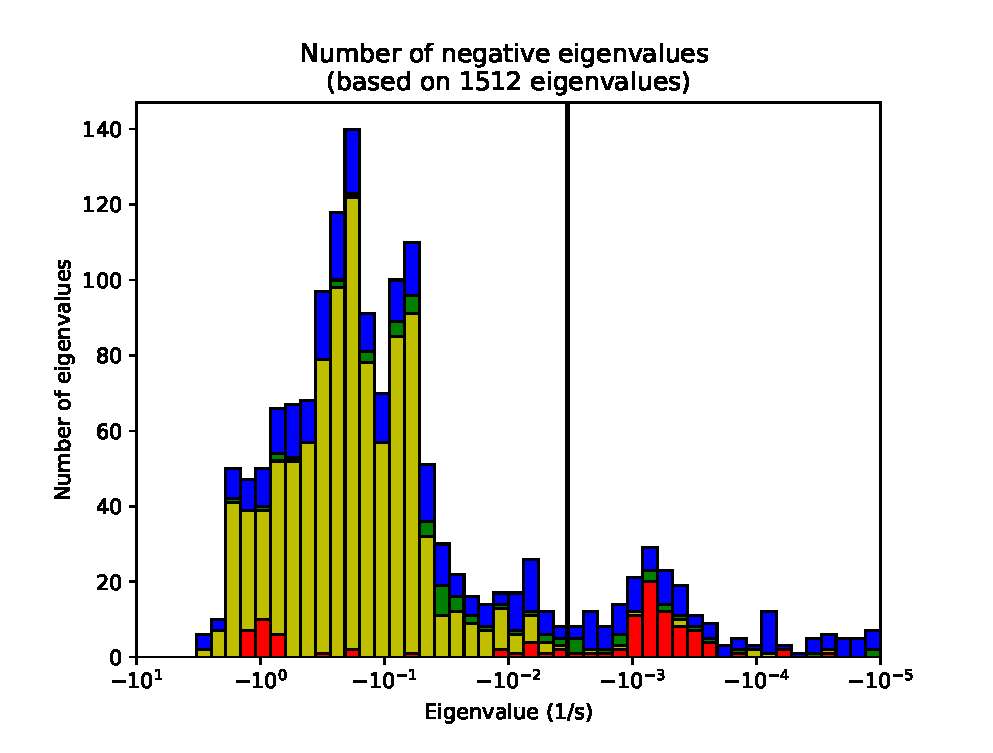
\includegraphics[width=6.5in]{./time_hist_all_values_neg_c6_subsample.eps}
  \caption[Histogram of negative eigenvalues of the Jacobian of MG2, focusing on a cluster of rain-producing grid cells]{Histogram of negative eigenvalues in cluster 6. Blue bars correspond to eigenvalues at grid points excluded from the subsample due to having active ice processes (\num{647} grid points). Green bars correspond to grid points excluded due to having active rain evaporation at the beginning of the time step (\num{118} grid points). Yellow bars correspond to the grid points excluded due to developing rain evaporation over the course of a time step (\num{3796} grid points). Red bars correspond to the grid points included in the subsample (\num{843} grid points). A black line is placed at $(\SI{300}{\second})^{-1}$ for comparison with the MG2 time step.}
  \label{eig-c6-subsample}
\end{figure}

Given this situation, we decided to use a second, broader subsample so as not to exclude points that develop rain evaporation. This corresponds to the yellow and red bars in Figure \ref{eig-c6-subsample}. For this broader subsample, substepping accretion and autoconversion alone would probably not be sufficient to adequately represent the rain mass overall, since rain evaporation also becomes an important process. However, we might hope that substepping accretion and autoconversion together would at least reduce error in the rain production rate, especially since most evaporation should occur after the cloud is depleted, when the accretion should be slowing down.

Unfortunately, this is not the case, as Figure \ref{convergence-accr-auto2} shows. There is significant error in the rain production rate unless all rain-related processes are substepped together. We note that first-order convergence happens below a time step of about \SI{20}{\second}. Figure \ref{eig-c6-subsample} suggests that we might need an even smaller time step, but in practice, this does not seem to make much difference. This may be because these eigenvalues were calculated based on the conditions at the beginning of the time step. After some time has elapsed, the evaporation is turned on, while the self-collection is likely to cause the particles to reach maximum size, at which point the self-collection effectively turns off. This represents an important feature of MG2 not captured by our linear approach; if the time step is reduced, then different processes may activate at different times, and the timescales associated with active processes may also change over time.

\begin{figure}[htbp]
  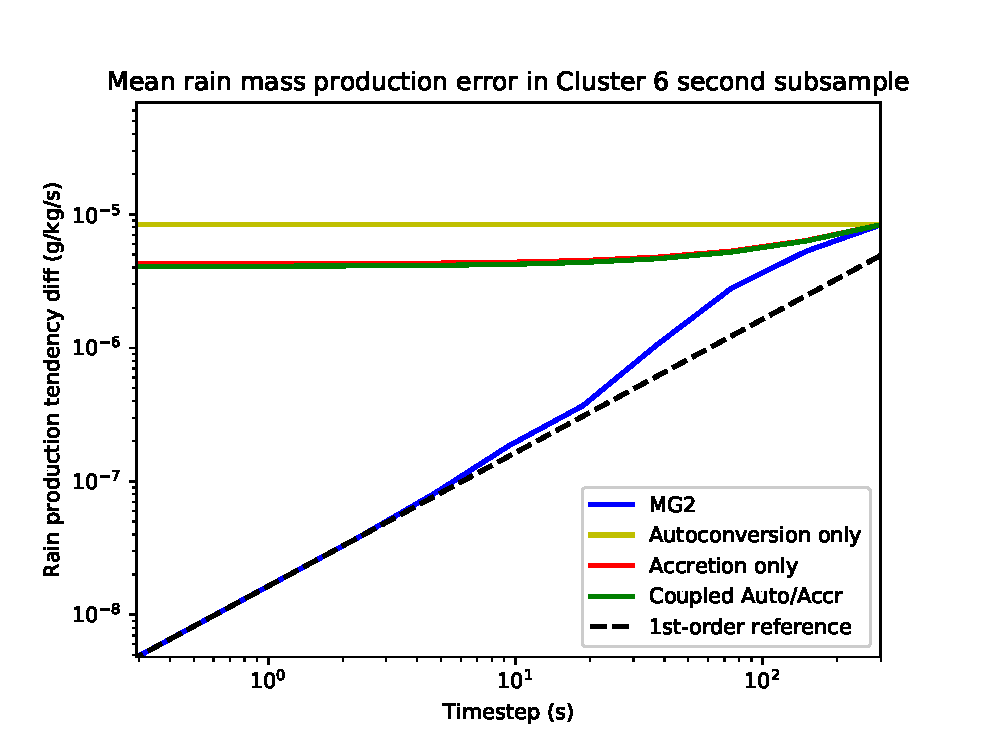
\includegraphics[width=6.5in]{./substep_convergence_prod_c6_initicefilter_richext.eps}
  \caption[Convergence plot for mean MG2 error in a subsample of a cluster of rain-producing grid cells using different substepping strategies]{Convergence plot for mean error in second cluster 6 subsample, under different substepping strategies for accretion and autoconversion. Instead of the total water mass difference, only the rate of rain production (autoconversion+accretion) is plotted. Runs substepping all of MG2 are shown in blue. Runs substepping accretion and autoconversion together, with total MG2 time step held fixed at \SI{300}{\second}, are shown in green. Substepping accretion alone is shown in red, and substepping autoconversion alone is shown in yellow. The dotted reference line has slope \num{1}.}
  \label{convergence-accr-auto2}
\end{figure}

It is worth noting that all results in this section are broadly consistent with the prior literature in that they suggest a time step size of \SI{60}{\second} or below is necessary to reduce the error to within a few percent of the total process rate. Notably, in the case of rain evaporation, the error hardly improves until the time step is on the order of tens of seconds or lower.

\section{Discussion} \label{sec:MG2-discussion}

Our analysis of MG2, based on examining the eigenvalues of a numerically-derived Jacobian, shows that there are many situations where MG2 would appear to be unstable when using a forward Euler method at a \SI{300}{\second} time step. It is stable in practice due to nonlinearities in MG2, and especially due to the presence of limiters, but we would expect these limiters to reduce the accuracy with which E3SMv1 solves the equations that MG2 is intended to implement.

This leads us to three concerns. First, is the time discretization error first-order, so that we can readily trade off increased computational cost for a proportional decrease in error? Or are there key unresolved timescales present in the system, so that the solutions we find at a \SI{300}{\second} time step are qualitatively different from the converged results? For instance, if certain process rates are typically constrained by limiters at long time steps, then modest improvements to the process rates will have little effect on the result, since both the original and ``improved'' process rates will be overwritten with the limited value. There will therefore be little benefit to reducing the time step until we reach the point where the model runs stably without these limiters.

Our results show that the default time step is adequate to resolve MG2's physics in some cases and not others. The time step needed by MG2 depends on the regime, and particularly on the set of processes that are active in that regime. The timescales involved in the production and growth of snow, for instance, seem to be generally much longer than the \SI{300}{\second} time step MG2 typically runs at. For processes involving rain or cloud ice, however, MG2 relies on limiters for stability, and in cases where rain evaporation is an important process, we have shown that the \SI{300}{\second} time step is an order of magnitude too large to achieve first-order convergence.

Our second concern is whether we can use a process-based analysis of MG2 to improve accuracy without substepping the entire microphysics. Our results again suggest that it is possible to considerably improve accuracy in this way in certain regimes, but that it takes some care to do so effectively. For instance, substepping MG2's rain evaporation at a much shorter time step, say \SI{10}{\second}, produces a large increase in model cost (it requires multiple calculations involving computationally-expensive exponential functions), yet this only moderately reduces the error. But by also substepping rain self-collection (a less computationally-intensive process) in the same loop, the error can be reduced by an order of magnitude. In general, it seems necessary to substep rain-related processes together, but it may be possible to do so without substepping the entire microphysics. We believe that sedimentation may also be relevant to these rain processes, and hope that a future study will investigate including rain evaporation, self-collection, and accretion as part of the sedimentation solver itself, rather than sequentially splitting sedimentation from the microphysical processes.

Third, we can broaden our view and ask whether resolving MG2's physics better would have a significant effect on model climate. To answer this question, we ran a simulation using E3SMv1 with MG2 substepped at a \SI{1}{\second} time step (compset F1850C5AV1C-04P2, grid ne30\_ne30) for four simulated years.

Figure \ref{e3sm-taylor} shows a Taylor diagram \parencite{Taylor2001} that compares the spatial variability of several key variables in this run to a control run with the MG2 default time step of \SI{300}{\second}. Taylor diagrams are polar plots that are typically used to summarize the differences between different simulations (or between a simulation and an observational data set). For each variable, the standard deviation is calculated in the modified simulation, and this is used to set the radius for the data point associated with the variable. The correlation between the variable in the modified run and the same variable in the control run is also calculated, and the inverse cosine of this value is used to set the angle where the point is plotted. A useful property of Taylor diagrams is that the \num{2}-norm (root mean square) of the difference between the modified and control data is proportional to the distance of each point from the reference point on the $x$ axis. In this case, the differences between the modified run and the control run are quite minor.

Figure \ref{e3sm-prect-comparison} shows the spatial distribution of total precipitation, which likewise is quite similar and shows no obvious systematic differences. We do note that the global mean stratiform precipitation from MG2 increases from \SI{1.23}{\milli\meter} to \SI{1.31}{\milli\meter} per day. However, the convective precipitation is reduced to a degree that almost exactly cancels this, from \SI{1.90}{\milli\meter} to \SI{1.83}{\milli\meter} per day.

We can see much larger differences if we look specifically at the vertical distribution of rain mass from MG2. Figure \ref{e3sm-rain-comparison} shows the difference between the zonally averaged in-area rain mass, which shows a reduction of rain in the upper cloud and near the surface, as well as an increase in the lower cloud. This is due to a combination of reduced production of rain, reduced rain evaporation, and the effects of these differences on the rain fall speed. In particular, if a reduction in rain evaporation in the cloud base is matched by an equal reduction in rain production within the cloud (both from the stratiform and convective schemes), that suggests that the model is not particularly sensitive to the rain evaporation rate, since the precipitation is governed largely by energetic constraints rather than such specific details of the microphysics. However, the exact mechanism for this feedback is not immediately clear; one could also easily imagine an alternative outcome where a change in rain process rates affects cloud properties enough to cause a significant change in the shortwave cloud forcing. We also believe that the coupling of sedimentation to these processes should be further examined.

\begin{figure}[htbp]
  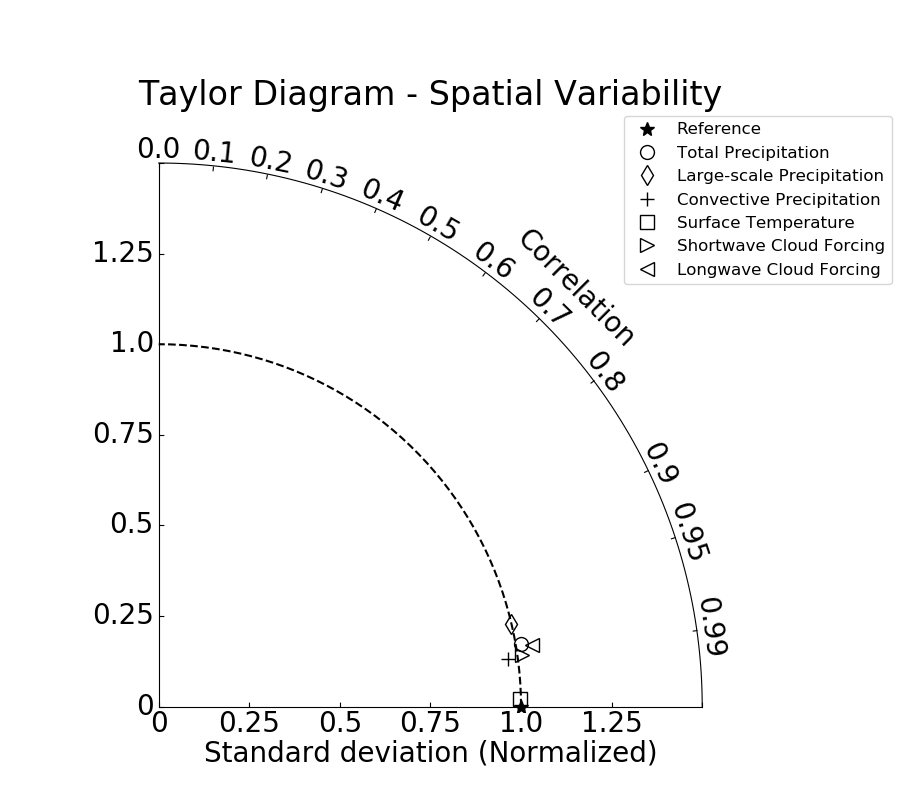
\includegraphics[width=6.5in]{./ANN_metrics_taylor_diag.png}
  \caption[Taylor diagram comparing an EAMv1 simulation with reduced MG2 substep to a control run]{Taylor diagram comparing run with MG2 running at \SI{1}{\second} to run at default settings. Only years \numrange{2}{4} of the simulation were used.}
  \label{e3sm-taylor}
\end{figure}

\begin{figure}[htbp]
  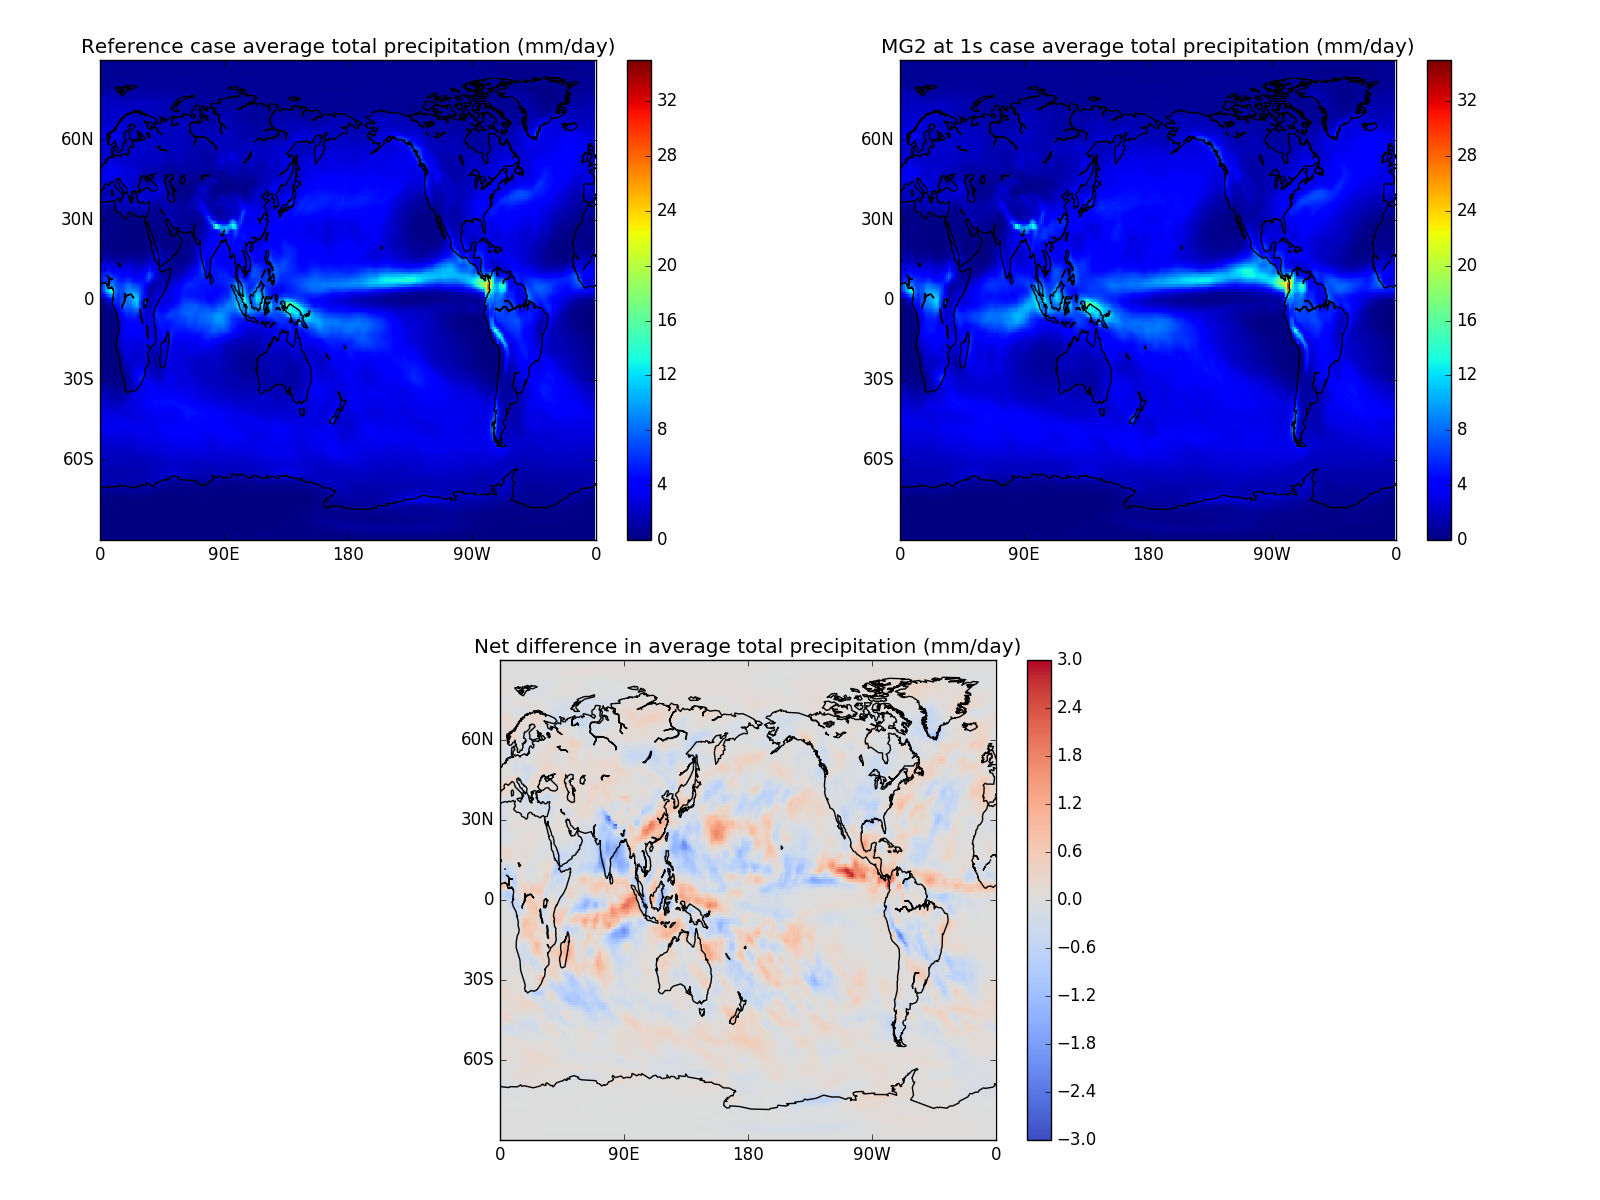
\includegraphics[width=6.5in]{./MG2Figure13.png}
  \caption[Comparison of total surface precipitation in EAMv1 simulations with different MG2 substep sizes]{Comparison of total precipitation at the surface using MG2 at a \SI{300}{\second} (left) and \SI{1}{\second} (right) time step over three years, with the difference also plotted (center).}
  \label{e3sm-prect-comparison}
\end{figure}

\begin{figure}[htbp]
  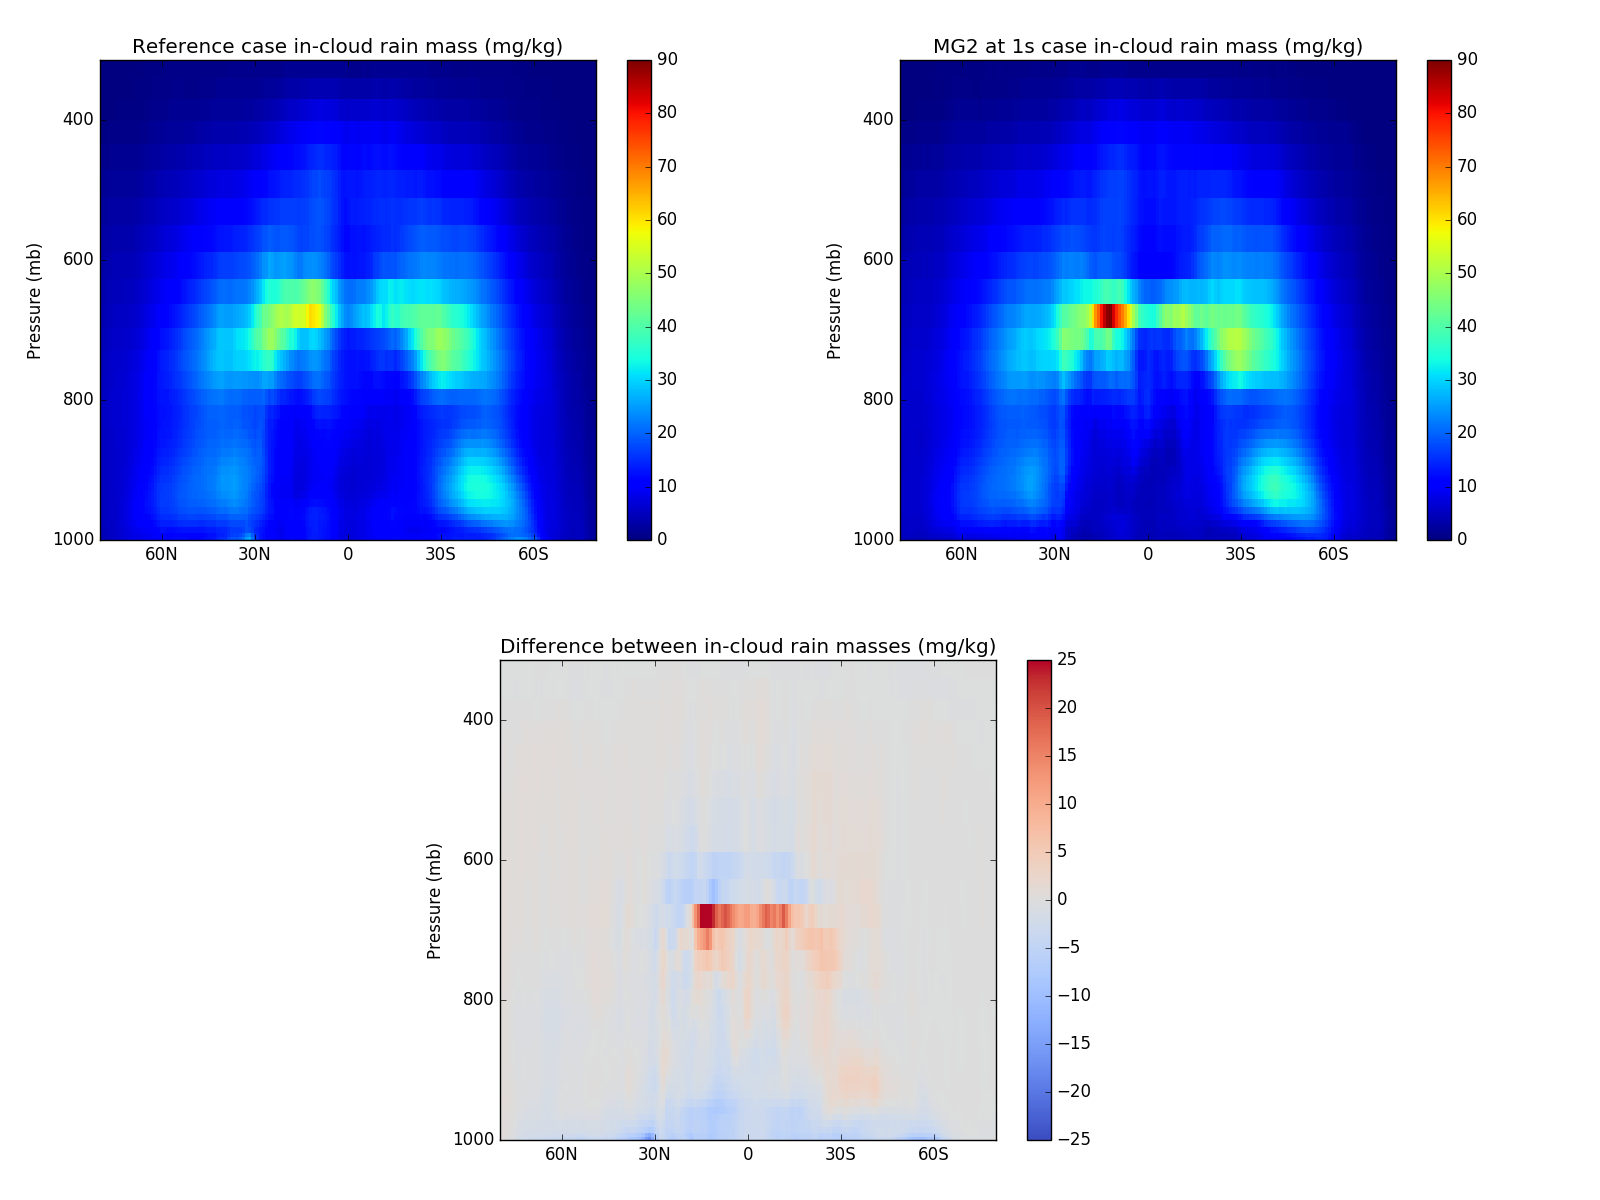
\includegraphics[width=6.5in]{./MG2Figure14.png}
  \caption[Comparison of zonally-averaged rain mass in EAMv1 simulations with different MG2 substep sizes]{Comparison of zonally-averaged rain mass in E3SMv1 runs using MG2 at \SI{300}{\second} (left) and \SI{1}{\second} (right) time step over three years, with the difference also plotted (center).}
  \label{e3sm-rain-comparison}
\end{figure}

These results with the global model present us with an interesting conundrum. Within MG2, we found that, while the rain evaporation rate was sensitive to the MG2 time step, substepping the rain evaporation by itself provided only a modest improvement in the evaporation rate. The coupling frequency between rain evaporation and self-collection was just as important a factor as the rain evaporation time step itself. By analogy, it's possible that accurately resolving MG2 process rates may require coupling MG2 with other parameterizations, rather than substepping the microphysics by itself.

Is this really the case, or is EAMv1 just not sensitive to these microphysical process rates? What time steps actually do impact model climate? To answer questions, we turn our attention in the next chapter to simulations using the full EAMv1 model.

\chapter{Process Coupling in the E3SM Atmosphere Model} \label{ch:EAM}

In this chapter, we discuss our study on changing time steps in global EAMv1 simulations. Section \ref{sec:EAM-background} will discuss results on time step sensitivity in related models. In section \ref{sec:EAM-methodology}, we will discuss the methodology of this study, and we will cover the outcomes of the study in section \ref{sec:EAM-results}. Section \ref{sec:EAM-discussion} will summarize these results and their implications for model development.

\section{Background} \label{sec:EAM-background}

Prior research using the CAM, versions 3 and 4, (CAM3/CAM4), as well as CAM's predecessor, the Community Climate Model, version 3, suggests that time step size for a GCM has significant effects on precipitation in an aquaplanet simulation, particularly in the intertropical convergence zone (ITCZ) \parencite{Williamson2003, Williamson2008, Mishra2008}. Decreasing the time step increases total precipitation in the ITCZ and the frequency of extreme precipitation events. The partition of precipitation between the large-scale and convective parameterizations is also affected, with an increase in the large-scale precipitation being responsible for the aforementioned effects. For CAM3, the increase in total precipitation was found to be dependent on an increase in evaporation at the surface, which in turn was due to an increase in wind speed and a decrease in specific humidity near the surface \parencite{Mishra2008}. Further research using CAM3 for real-planet simulations confirmed these results, and showed that the increased evaporation, in addition to producing increased precipitable water (and precipitation), also produced a larger cloud fraction at low altitude and an increased magnitude of radiative cloud forcing \parencite{Mishra2011}. \textcite{Williamson2013}, using CAM4, found that the time step of the convective schemes, and in particular their rate of coupling with other processes, controlled the repartitioning of precipitation between large-scale and convective processes.

\textcite{Yu2015} experimented with changes in the global model time step for a superparameterized version of CAM3 (SPCAM3), without changing its cloud resolving model's time step. Decreasing the CAM time step increased overall precipitation in SPCAM3, as well as the frequency of heavy precipitation events, which also happened for CAM3. However, reducing the time step size in SPCAM3 \emph{decreased} precipitable water, decreased both liquid and ice water path, and ultimately decreased the magnitude of radiative cloud forcings. This was hypothesized to be due to changes in convective organization, producing an increase in precipitation efficiency and effectively drying out the atmosphere.

Although both CAM3 and SPCAM3 experience similar increases in surface evaporation and precipitation (which must match in the long run, to balance the water budget), the proposed mechanisms driving these changes are different. In effect, the increased evaporation in CAM3 ``pushes'' more precipitable water into the atmosphere, eventually forcing an increase in condensation and precipitation to remove this water, while the increased precipitation efficiency in SPCAM3 ``pulls'' water out of the atmosphere, drying it out and encouraging evaporation to replace the lost water.

EAMv1 shares very little of its physics with CAM3, and almost none with SPCAM3. Nevertheless, EAMv1 uses the same general strategies for coupling the physics parameterizations, dynamics, and surface components. Although our study on MG2 found that the total precipitation was not very sensitive to changes to the MG2 time step alone, we did see a mild increase in the ratio of stratiform to convective precipitation, consistent with the CAM3 and SPCAM3 results. We therefore expected that our experiments with changing the time step of the full model would show some of the same effects on precipitation rates seen in CAM3 and SPCAM3.

Unlike earlier models, EAMv1 has the ability to easily substep two of the main cloud physics parameterizations, CLUBB and MG2, besides changing the overall physics time step. The radiative transfer and dynamics can also be adjusted independently from the dynamics-physics coupling interval. This provides an opportunity to perform a series of controlled experiments on time step sensitivity in EAMv1's cloud and precipitation-related variables. By independently changing these various time steps, we could observe whether EAMv1 is most sensitive to the time step used to integrate specific physical processes, or to the coupling frequency between particular sets of processes.

\section{Methodology} \label{sec:EAM-methodology}

We ran E3SMv1 at a $\sim$\SI{100}{\kilo\meter} atmospheric resolution (ne30\_ne30 grid) with standard E3SMv1 tuning and prescribed sea surface temperature. These runs were performed using a maintenance version of E3SM 1.1 (hash 25c94366) with pre-industrial forcings (compset F1850C5AV1C-04P2) unless otherwise specified, and all had prescribed sea surface temperature (SST) and sea ice extent.

The control run (CTRL) is an out-of-the-box run using default settings. We compare this to a new run (ALL10) that changed the atmosphere's dynamics-physics-surface coupling time step, known as ``dtime'' in the model settings, to \SI{10}{\second}. This time step is chosen to be as small as we could reasonably afford, within the constraints of the computing power we had available for this study. CTRL and ALL10 simulations are both \num{3} years in length. Results based on years \numrange{1}{2} were unchanged after adding year \num{3}, which gives us confidence that \num{3} years is long enough to draw robust conclusions.

The dtime setting is often thought of as specifying the entire atmosphere's time step, but there are three ways in which this is not quite true. First, the radiation parameterization uses a fixed time step of once per hour, regardless of dtime. While the ALL10 run does not modify the radiation time step, our tests with shorter runs show that the model is not especially sensitive to this time step. Second, the dynamics and cloud physics contain some substepping by default, though none run at a time step as small as \SI{10}{\second}. In the ALL10 run, we disable these forms of substepping, so that all major dynamics and physics processes aside from radiation run at the same small time step. Third, because the dtime setting also governs the rate at which EAMv1 exchanges information with the surface components, changing it forces a change in the land and sea ice components, which must run at a \SI{10}{\second} time step as well.

To investigate which processes within EAMv1 were most responsible for its overall time step sensitivity, we configured a series of runs using built-in options to substep individual parameterizations at a \SI{10}{\second} time step. These runs include DYN10, which substepped EAMv1's spectral element dynamical core, CLUBB10, which substepped the CLUBB cloud physics parameterization, and MICRO10, which substepped the MG2 stratiform microphysics. Typically CLUBB and MG2 are substepped together within a single loop, so we also produced a CLUBBMICRO10 run that used this capability to run both schemes at \SI{10}{\second}. Because this run showed clear differences from the control, we produced a CLUBBMICRO60 run where CLUBB and MG2 were substepped together at \SI{60}{\second}. Separately, we also produced a CLUBB10MICRO10 run, where the individual time steps for CLUBB and MG2 were reduced, but the two schemes were only coupled at the default rate of once per \SI{300}{\second}. To verify our prior belief that the model is less sensitive to the radiative transfer time step than to other physics time steps, we produced the ALLRAD10 run, which is identical to the ALL10 run except that the radiation is also run at a \SI{10}{\second} time step. Finally, we produced the ALL300 and ALL60 runs, which change dtime to \SI{300}{\second} and \SI{60}{\second}, respectively. ALL300 is useful as an additional control, because it decreases the dynamics-physics coupling time step, but does not decrease the CLUBB or MG2 time steps, nor does it decrease the dynamics time steps (except the remapping for the vertically Lagrangian advection scheme, which normally runs every \SI{900}{\second}). A summary of all these runs can be found in Table \ref{tab:runs}.

\begin{table}
  \centering
  \footnotesize
  \begin{tabular}{|c|p{0.4\linewidth}|r|r|}
    \hline
    Name & Substepped processes & Substep size & Run length \\
    \hline
    CTRL & None & N/A & \SI{38}{\month} \\
    \hline
    ALL10 & Dynamics-physics coupling & \SI{10}{\second} & \SI{38}{\month} \\
    ALL60 & & \SI{60}{\second} & \SI{30}{d} \\
    ALL300 & & \SI{300}{\second} & \SI{30}{\day} \\
    \hline
    DYN10 & Dynamics and tracer advection & \SI{10}{\second} & \SI{30}{\day} \\
    \hline
    MICRO10 & MG2 microphysics & \SI{10}{\second} & \SI{30}{\day} \\
    \hline
    CLUBB10 & CLUBB unified cloud parameterization & \SI{10}{\second} & \SI{30}{\day} \\
    \hline
    CLUBB10MICRO10 & CLUBB and MG2 & \SI{10}{\second} & \SI{30}{\day} \\
    \hline
    CLUBBMICRO10 & CLUBB+MG2 combined loop & \SI{10}{\second} & \SI{30}{\day} \\
    CLUBBMICRO60 & & \SI{60}{\second} & \\
    \hline
    ALLRAD10 & Dynamics-physics coupling and radiation & \SI{10}{\second} & \SI{30}{\day} \\
    \hline
  \end{tabular}
  \caption{Runs performed using the default aerosol scheme.}
  \label{tab:runs}
\end{table}

In EAMv1, the most important parameterization that does \emph{not} have this built-in substepping capability is the ZM deep convection, which always runs at the time step given by dtime. Substepping this parameterization individually is challenging and is described further in section \ref{sec:zm-substep}.

\section{Results} \label{sec:EAM-results}

\subsection{Effects of Decreasing the Physics Time Step}

Consistent with the literature on CAM, we find a \SI{0.08}{\milli\meter\per\day} increase in global-mean total precipitation with \SI{10}{\second} time steps, mostly stemming from low latitudes. While convective precipitation decreases, large-scale precipitation increases by $\sim$\SI{60}{\percent} in the tropics (defined here as latitudes from \num{30}S to \num{30}N), especially over land (Figure \ref{fig:all10-prec-map}a). The overall effect is an increase in tropical precipitation over the Pacific warm pool, and a near-doubling of precipitation in parts of Borneo, New Guinea, and Colombia (Figure \ref{fig:all10-prec-map}b). We also note an increase in heavy precipitation, seen in Figure \ref{fig:all10-prec-intensity} as a shift towards more precipitation falling in extreme precipitation events. This shift is again due primarily to an increase in heavy large-scale precipitation and a decrease in convective precipitation (not shown).

\begin{figure}
    \centering
    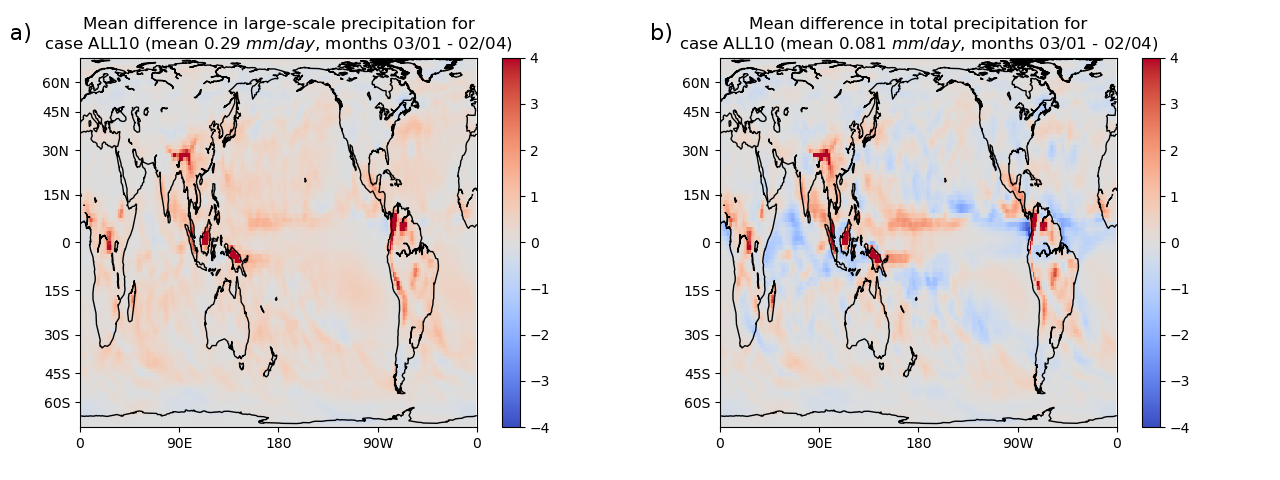
\includegraphics[width=6.5in]{Figure1.png}
    \caption[Differences in large-scale and total precipitation between CTRL and ALL10]{Differences in a) large-scale precipitation and b) total precipitation between CTRL and ALL10 runs.}
    \label{fig:all10-prec-map}
\end{figure}

\begin{figure}
    \centering
    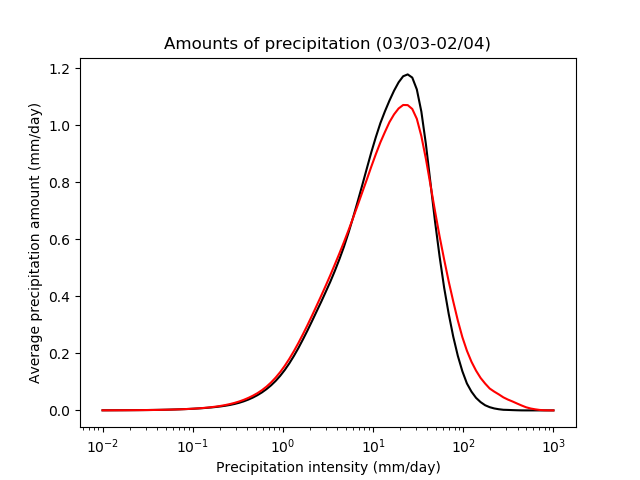
\includegraphics[width=6.5in]{PRECT_amount_y03m03-y04m02.png}
    \caption[Comparison between CTRL and ALL10, of amount of precipitation falling as a function of intensity of precipitation events]{Global mean of the average amount of rain produced by precipitation falling at a given rate, produced from hourly data from CTRL (black) and ALL10 (red). Amount is normalized so that an integral over the natural logarithm of precipitation intensity yields total global mean precipitation amount.}
    \label{fig:all10-prec-intensity}
\end{figure}

Evaporation must increase to fuel the precipitation increases.  Over the oceans, this is due to slightly higher wind speed and lower near-surface relative humidity. The average \SI{10}{\meter} wind speed in the tropics increases from \SIrange{5.56}{5.70}{\meter\per\second}, and occurs mainly in the northern Indian ocean and central Pacific, while latent heat flux increases in the same areas, by about \SI{4}{\watt\per\meter\squared} (not shown). This is consistent with the CAM3 literature, suggesting that an increase in wind speed contributes an increase in evaporation for short time steps.

Unlike in CAM3, the relative humidity decreases throughout the troposphere in the ALL10 run, as shown in Figure \ref{fig:all10-relhum-map}. The decreases in the \SIrange[range-phrase=--,range-units=single]{800}{850}{\millibar} layer correspond to a significant reduction in low cloud mass (Figure \ref{fig:all10-wp-map}). This suggests that the increase in precipitation is caused primarily by increased precipitation efficiency. At the same time, we see an increase in cloud liquid above the boundary layer, particularly at high latitudes. In the ALL10 run, the cloud fraction not only decreases at lower levels, where less liquid cloud is present, but also at higher levels, where the average cloud mass mixing ratios are similar to or greater than their values in CTRL (Figure \ref{fig:all10-cld-map}).

\begin{figure}
    \centering
    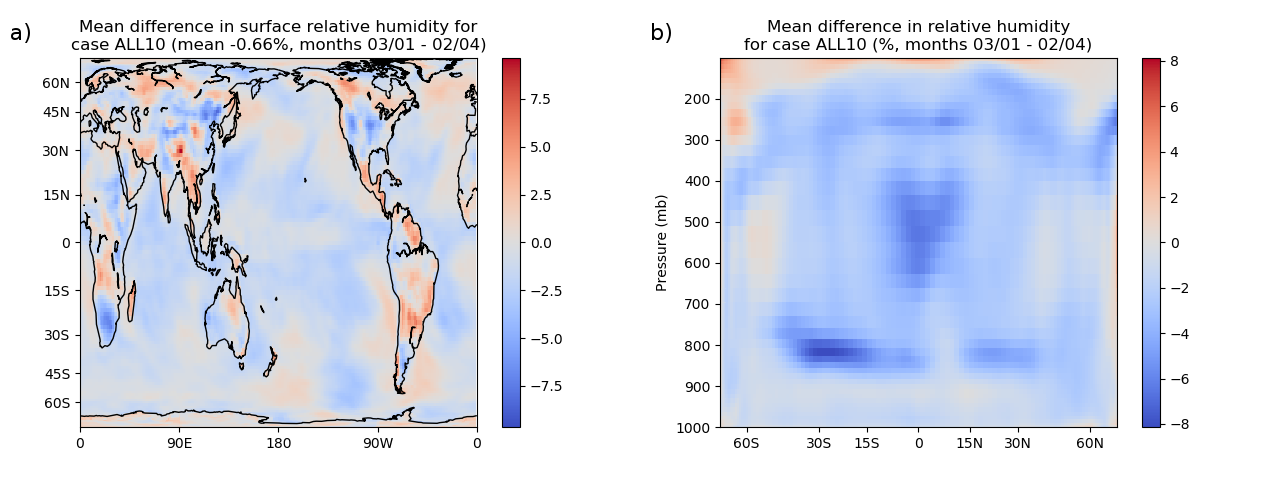
\includegraphics[width=6.5in]{Figure2.png}
    \caption[Differences in relative humidity between CTRL and ALL10 runs]{Differences in a) surface relative humidity and b) zonal mean relative humidity between CTRL and ALL10 runs.}
    \label{fig:all10-relhum-map}
\end{figure}

\begin{figure}
    \centering
    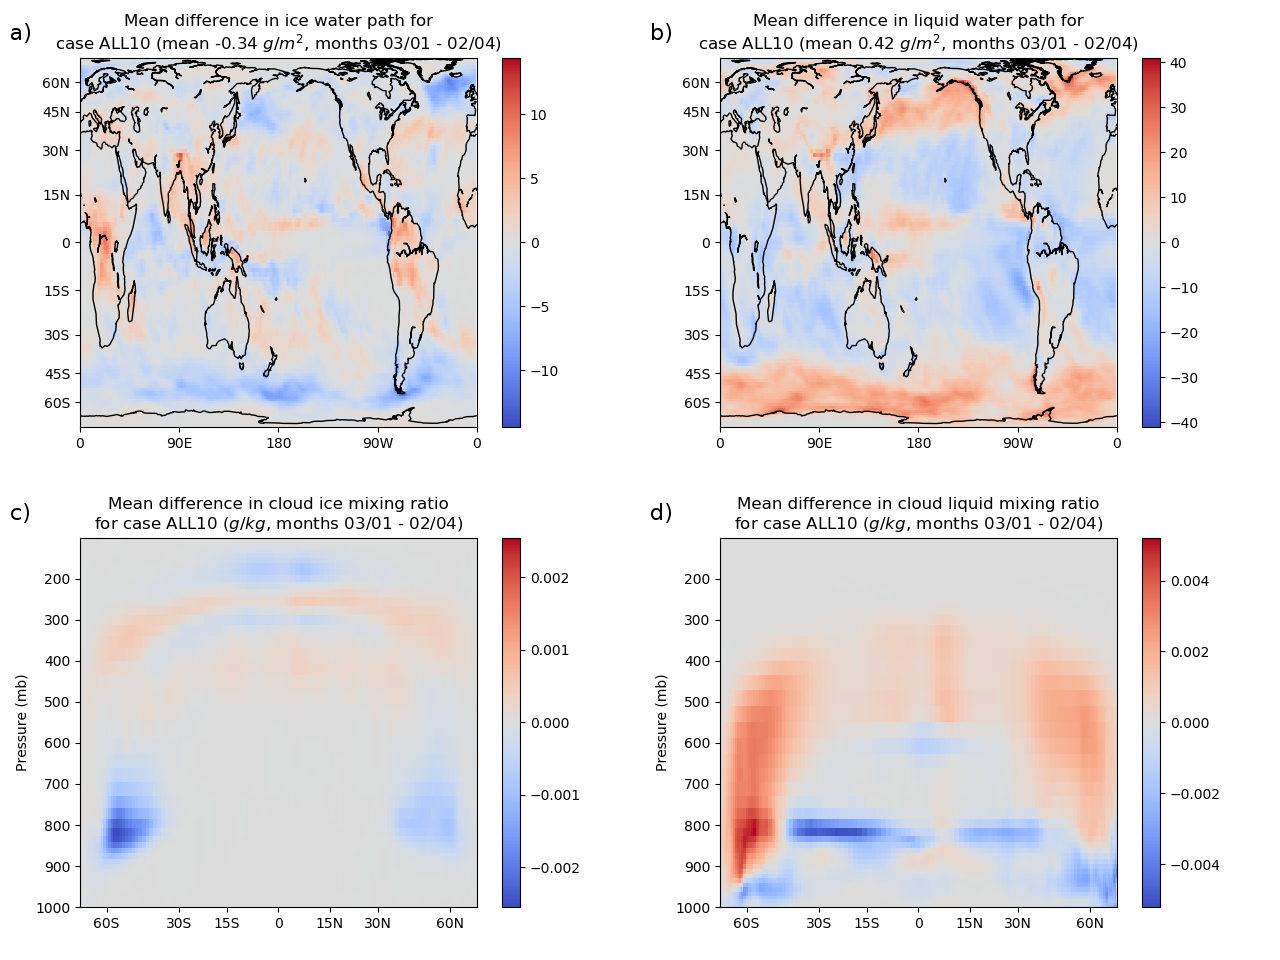
\includegraphics[width=6.5in]{Figure3.png}
    \caption[Differences in cloud mass between CTRL and ALL10 runs]{Differences in mass of cloud ice and liquid water between CTRL and ALL10 runs, measured by a) ice water path, b) liquid water path, c) zonal mean cloud ice mixing ratio, and d) zonal mean cloud liquid mixing ratio.}
    \label{fig:all10-wp-map}
\end{figure}

\begin{figure}
    \centering
    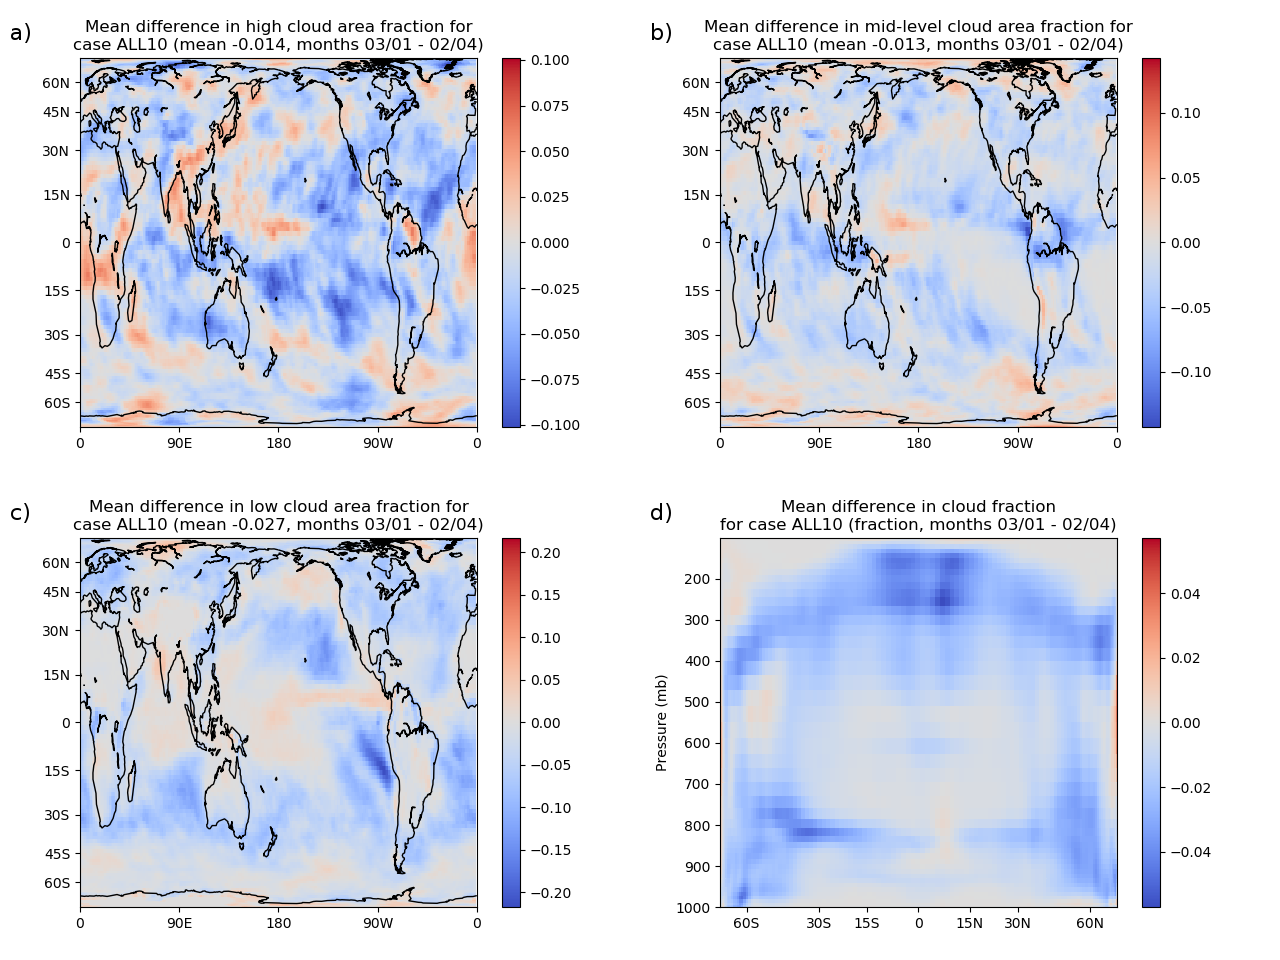
\includegraphics[width=6.5in]{Figure4.png}
    \caption[Differences in cloud fraction between CTRL and ALL10 runs]{Differences in cloud fraction between CTRL and ALL10 runs: a) high cloud fraction (defined as the vertical integral above \SI{400}{\millibar}), b) mid-level cloud fraction (vertical integral over the range \SIrange[range-phrase=--,range-units=single]{400}{700}{\millibar}), c) low cloud fraction (vertical integral below \SI{700}{\millibar}), and d) zonal mean cloud fraction at each level.}
    \label{fig:all10-cld-map}
\end{figure}

Consistent with the decrease in overall cloud mass and fraction, the ALL10 run shows substantially reduced radiative cloud forcing compared with CTRL, as can be seen in Figure \ref{fig:all10-cf-map}. The effect on shortwave cloud forcing is especially large, the global mean being reduced from \SI{-43.0}{\watt\per\meter\squared} to \SI{-37.5}{\watt\per\meter\squared}.

\begin{figure}
    \centering
    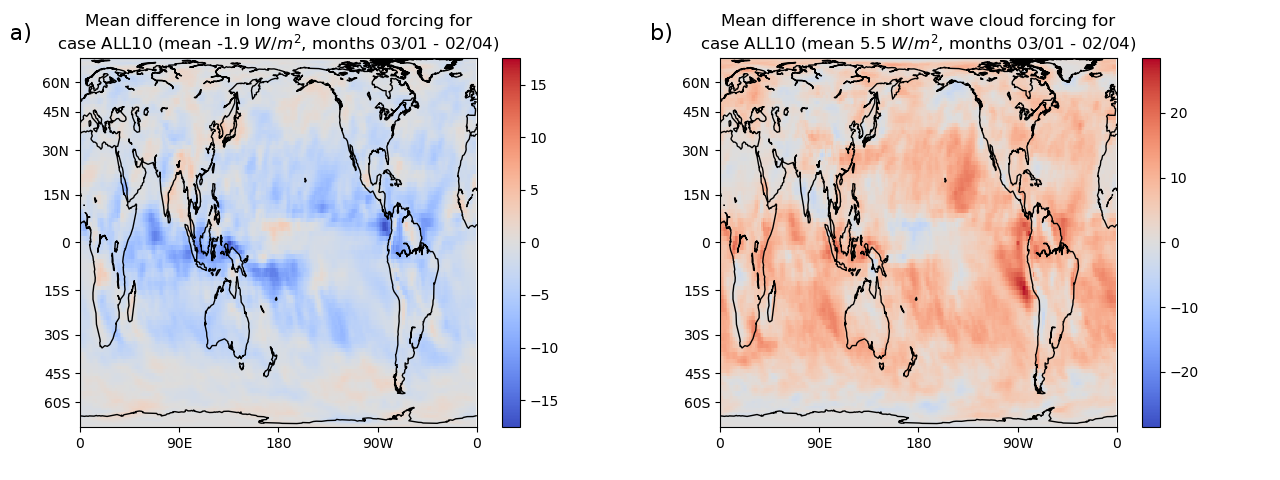
\includegraphics[width=6.5in]{Figure5.png}
    \caption[Differences in radiative cloud forcing between CTRL and ALL10 runs]{Differences in a) longwave cloud forcing and b) shortwave cloud forcing between CTRL and ALL10 runs.}
    \label{fig:all10-cf-map}
\end{figure}

Spatial-pattern differences between CTRL and ALL10 are summarized by a Taylor diagram shown in Figure \ref{fig:taylor}. We find that the effect of reducing the model time step to \SI{10}{\second} (black symbols) is comparable to the effect of doubling the model's horizontal grid spacing (red symbols), a natural standard for comparison. Historically, spatial resolution changes have been perceived as a major model change while accompanying time step changes have been taken for granted; Figure \ref{fig:taylor} illustrates that this viewpoint has shortcomings. The variables most affected by the time step are related to precipitation, with the large-scale precipitation showing the most difference.

\begin{figure}
    \centering
    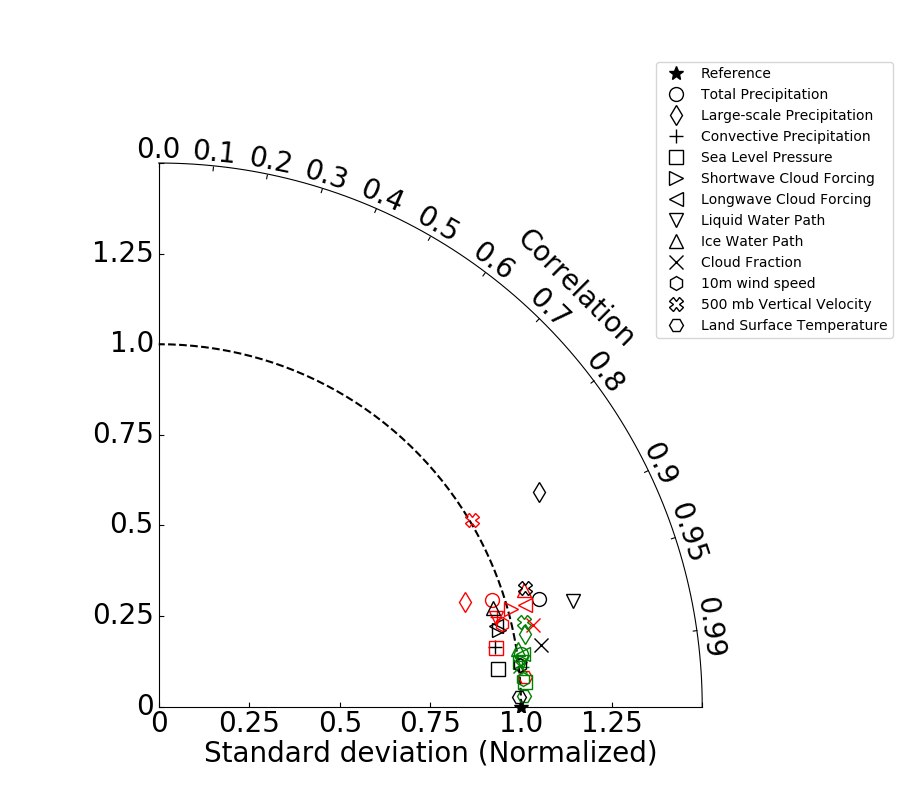
\includegraphics[width=6.5in]{ANN_metrics_taylor_diag_timesteps.png}
    \caption[Taylor diagram comparing EAMv1 simulations at varying spatial and temporal resolution]{Taylor diagram comparing results from the CTRL and ALL10 runs (black), and comparing results from CTRL to a run with default settings using the ne16 grid (red), which has a grid spacing of $\sim$\ang{1.9}. For these runs, we use values averaged over a three year time period starting March of the first simulated year. We also extend CTRL by an additional three years, and plot a comparison of those three years to the original three (green), to demonstrate that correlation is much higher if no change to spatial or temporal resolution are made. Only spatial variability is accounted for in this diagram.}
    \label{fig:taylor}
\end{figure}

\subsection{Effects of Changing the Physics Substepping}

We did not have the computational resources to run all of our substepped configurations for multiple years, but many of the effects of substepping are quite large and can easily be distinguished with only a few days of data. Since all runs started with the same initial conditions, they followed a similar trajectory for the first \num{15} days before beginning to diverge, so we focused on comparing the runs during this time period. (In Figure \ref{fig:cld-frc}, we have included data from \num{30} days, which shows an example of how, in these different runs, the global means of cloud-related variables become significantly less correlated towards the end of the month.)

We first examine the changes in precipitation across these runs, shown in Figure \ref{fig:precl-prect}. We can categorize our runs into five main categories based on large-scale precipitation:

\begin{enumerate}
\item The lowest average large-scale precipitation rates are found in CTRL, CLUBB10, and DYN10, suggesting that the cloud physics is not sensitive to the CLUBB or dynamics time steps.
\item A slightly higher large-scale precipitation rate is found in the ALL300 run, which has a reduced time step for the ZM deep convection and an increased dynamics-physics coupling frequency, but does not change the CLUBB or MG2 time steps. This run shows a mild repartitioning of precipitation from the convective to large-scale category, perhaps consistent with the mechanisms described in \textcite{Williamson2013}.
\item The MICRO10 and CLUBB10MICRO10 runs show signs of increased precipitation efficiency overall, increasing both large-scale \emph{and} total precipitation.
\item One of the largest large-scale precipitation rates comes from CLUBBMICRO10, which couples CLUBB to MG2 every \SI{10}{\second}, suggesting that an increase in CLUBB-MG2 coupling frequency has an additional effect beyond that from simply substepping MG2 more frequently. CLUBBMICRO60 may see a similar effect, though it is not as clearly distinguished from the MICRO10 run.
\item The ALL10 and ALLRAD10 runs decrease both the dynamics-physics coupling time step and the time step used for all physics parameterizations, and these show the largest changes in precipitation.
\end{enumerate}

\begin{figure}
    \centering
    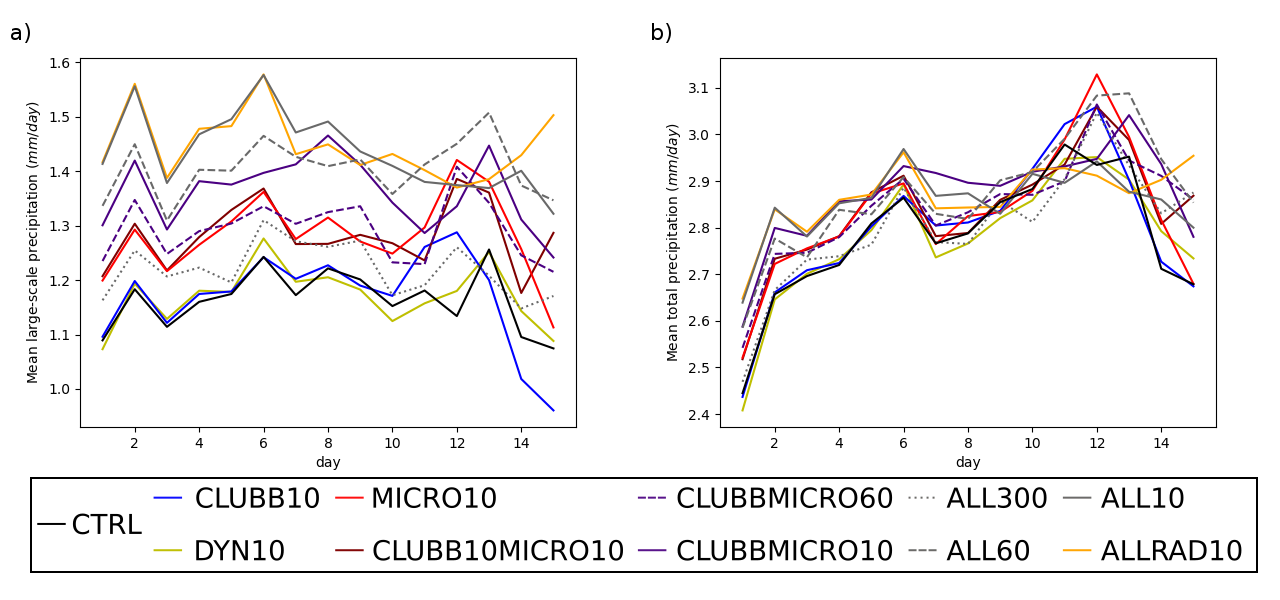
\includegraphics[width=6.5in]{Figure7.png}
    \caption[Rates of large-scale and total precipitation over time for short EAMv1 runs using different forms of substepping]{Daily global means of a) large-scale precipitation only and b) total precipitation for substepped runs.}
    \label{fig:precl-prect}
\end{figure}

The increase in extreme precipitation events, shown in Figure \ref{fig:prec-intensity}, is only clearly distinguishable in runs from the second, fourth, and fifth of these categories, implying that this increase is partly due to the CLUBB and MG2 joint time step, and partly due to the effect of reducing dtime, with MG2's time step by itself playing little or no role.

\begin{figure}
    \centering
    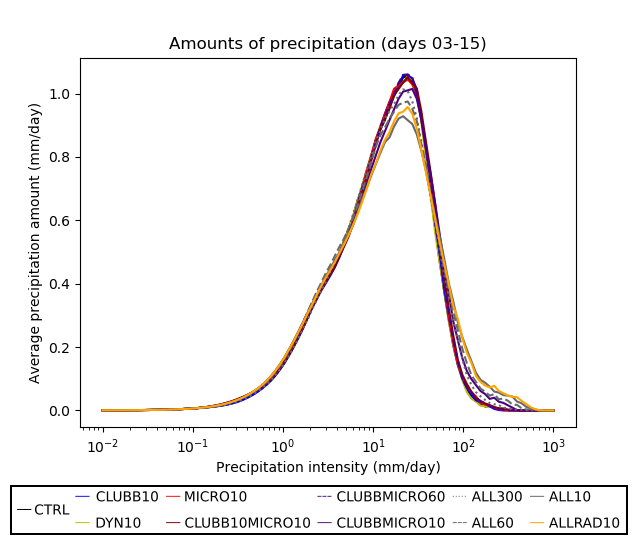
\includegraphics[width=6.5in]{PRECT_amount_d03-d15_legend.png}
    \caption[Comparison between short EAMv1 runs with different substepping, of amount of precipitation falling as a function of intensity of precipitation events]{Global mean of the average amount of rain produced by precipitation falling at a given rate, produced from hourly data from substepped runs, days 3--15. Amount is normalized so that an integral over the natural logarithm of precipitation intensity yields total global mean precipitation amount.}
    \label{fig:prec-intensity}
\end{figure}

While the increase in large-scale precipitation seen in the MICRO10 run is substantial, the spatial pattern is quite different from the ALL10 case, as seen in Figure \ref{fig:precl-map}. In particular, the patterns observed in the ALL10 case, such as the increase in large-scale precipitation over land, only appear when both CLUBB and MG2 are substepped together, as in the CLUBBMICRO10 case. We have also plotted the CLUBB10MICRO10 case, to show that this difference is not due simply to the reduction in the CLUBB time step alone.

\begin{figure}
    \centering
    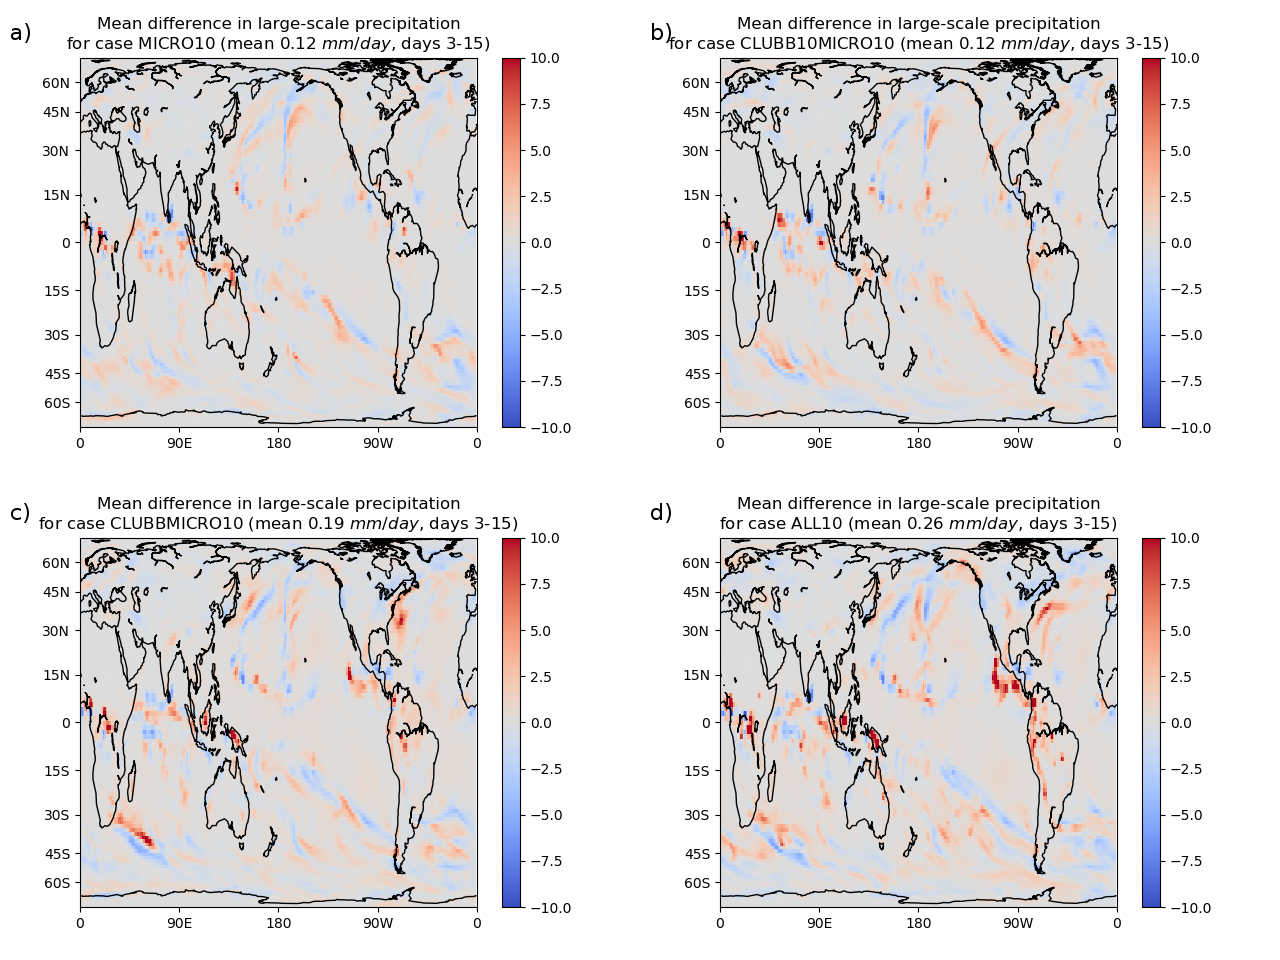
\includegraphics[width=6.5in]{Figure8.png}
    \caption[Differences in large-scale precipitation rates between short EAMv1 runs using different forms of substepping]{Differences in large-scale precipitation versus CTRL for a) MICRO10, b) CLUBB10MICRO10, c) CLUBBMICRO10, and d) ALL10.}
    \label{fig:precl-map}
\end{figure}

Together, these results suggest that the main time steps affecting the precipitation are the MG2 microphysics time step and the coupling time step between the CLUBB and MG2 schemes. The change in the CLUBB and MG2 combined time step therefore explains most of the precipitation change noted earlier between the CTRL and ALL10 runs. Either the dynamics-physics coupling time step or the ZM deep convection time step could also be affecting the precipitation between the convective and large-scale processes, since both these time steps are changed in the ALL10 and ALL300 runs. We will investigate this further in section \ref{sec:zm-substep}. The changes in total precipitation are mostly apparent for the first week of the run, after which the runs with default MG2 time step see a significant increase in convective precipitation (not shown), leading to no systematic difference between simulations after this point.

The particular pattern of decreased relative humidity found in the ALL10 run also appears in the CLUBBMICRO10 run, but not the MICRO10 run (not shown). However, as shown in Figure \ref{fig:cldliq-map}, the cloud liquid in the CLUBBMICRO10 run only matches the ALL10 run at low altitudes, while the ALL300 run is much more effective at matching ALL10 at higher altitudes, suggesting that the dynamics-physics coupling time step is responsible for these increases in cloud liquid. The CLUBBMICRO10 also consistently produces clouds in the lowest level of the atmosphere over land, particularly in South America and Southeast Asia, which are not seen in any other run. This may be an artifact resulting from CLUBB and MG2 running at a time step much smaller than the atmosphere-land coupling interval.

\begin{figure}
    \centering
    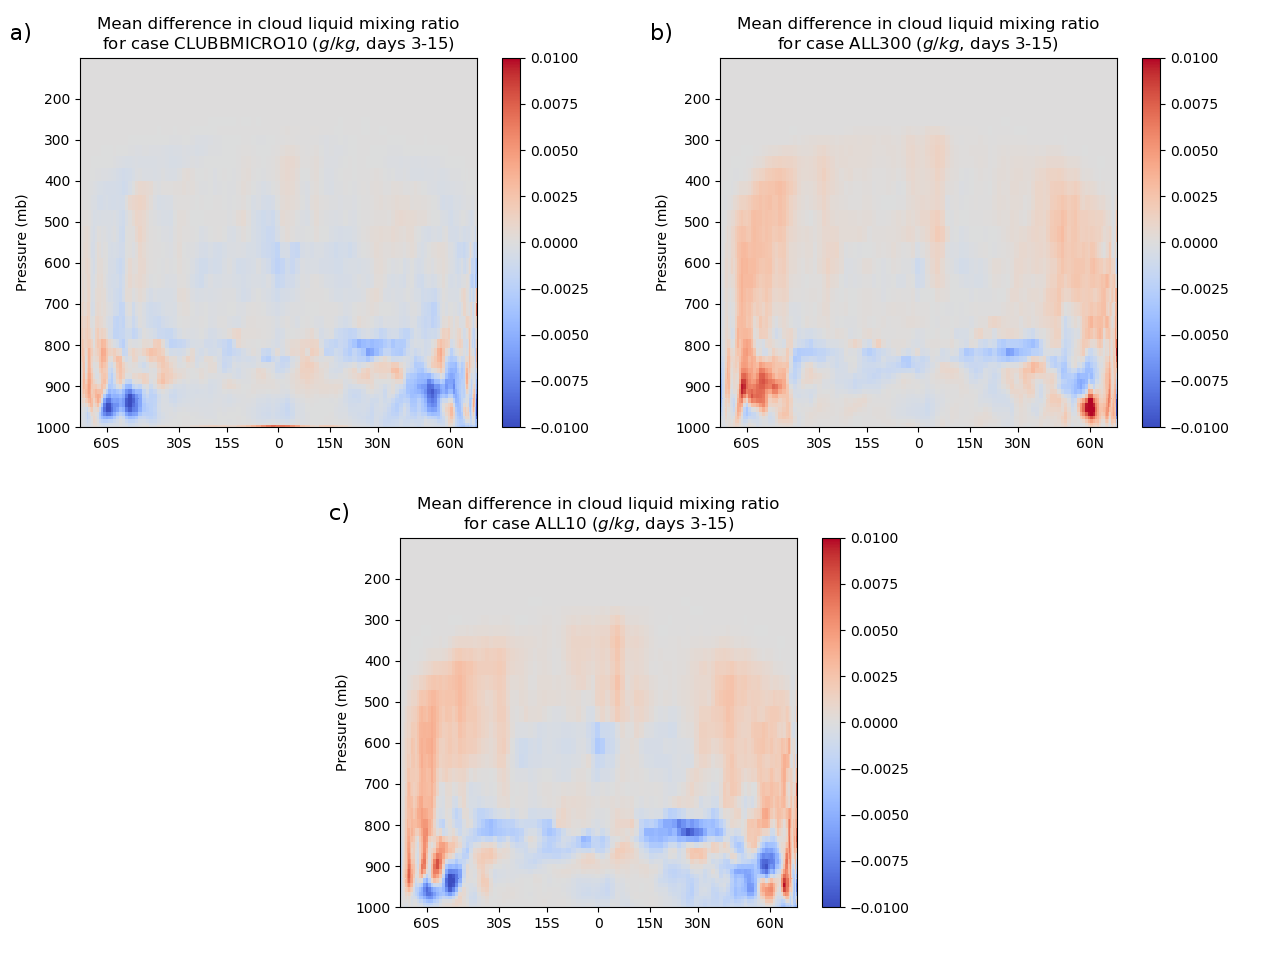
\includegraphics[width=6.5in]{Figure9.png}
    \caption[Differences in zonal mean cloud liquid mixing ratio between short EAMv1 runs using different forms of substepping]{Differences in zonal mean cloud liquid mixing ratio versus CTRL for a) ALL300, b) CLUBBMICRO10, and c) ALL10.}
    \label{fig:cldliq-map}
\end{figure}

The overall differences in ice and liquid water path are shown in Figure \ref{fig:water-path}. We see that, in the tropics, the runs with reduced MG2 time step reduce the liquid water path in a way that is similar to the ALL10 run, while the ALL300 run increases the ice and liquid water path everywhere. We also note that if MG2 is substepped independently from CLUBB, the ice water path increases significantly, but this does not occur when MG2 and CLUBB are substepped together.

\begin{figure}
    \centering
    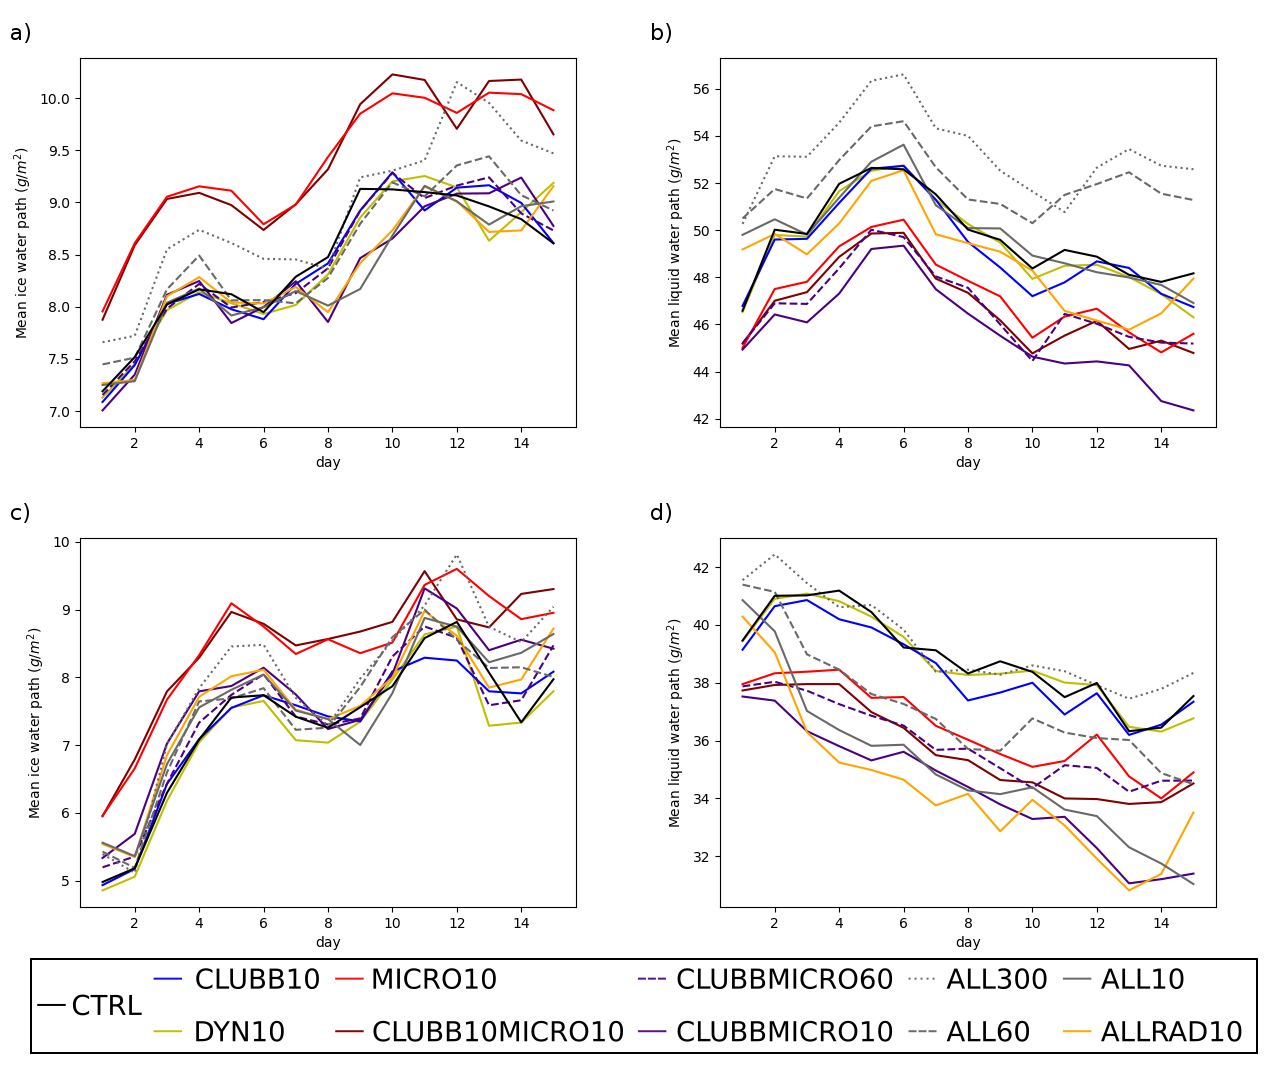
\includegraphics[width=6.5in]{Figure10.png}
    \caption[Cloud ice and liquid water paths over time for short EAMv1 runs using different forms of substepping]{Daily means for a,c) ice water path and b,d) liquid water path for substepped runs. Plots a-b) show global means, while c-d) show means over low latitude grid points (\num{30}S--\num{30}N).}
    \label{fig:water-path}
\end{figure}

We noted earlier that the ALL10 run caused a reduction in cloud fraction throughout most of the atmosphere, especially in the low cloud fraction. As shown in Figure \ref{fig:cldlow-cldmed}, this effect seems to have different causes, depending on which level of the atmosphere is examined. Reductions in low cloud are primarily due to the reduction in the dynamics-physics coupling substep, but the CLUBB and MG2 combined time step has a greater effect on the cloud fraction above \SI{700}{\millibar}.

\begin{figure}
    \centering
    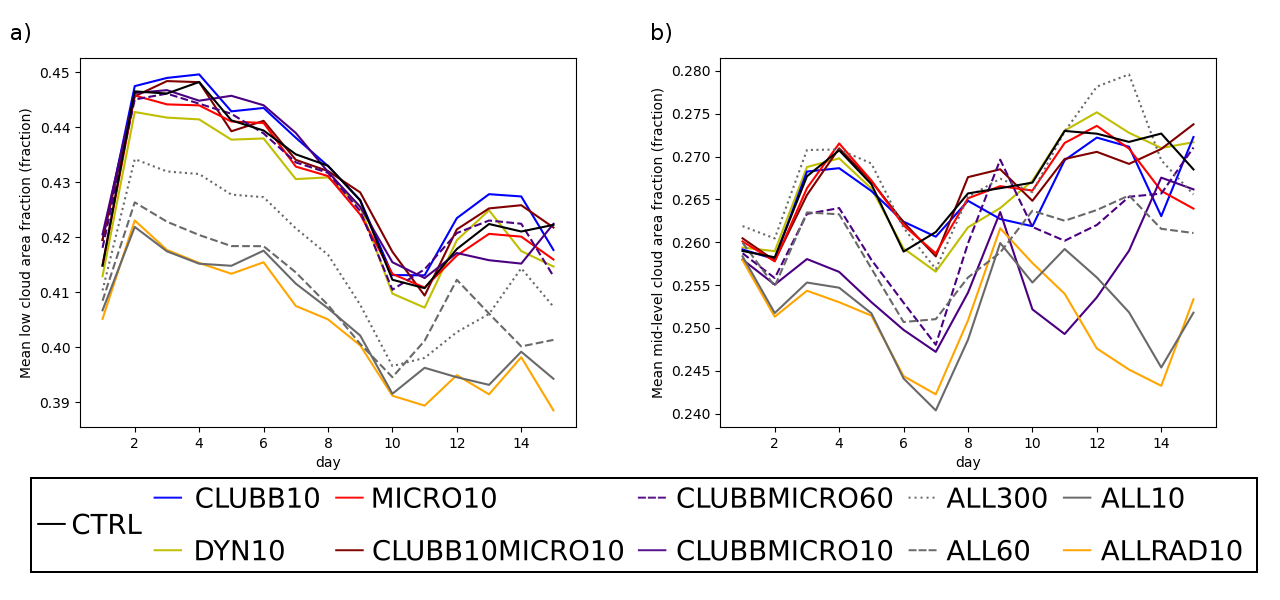
\includegraphics[width=6.5in]{Figure11.png}
    \caption[Low and mid-level cloud fractions over time for short EAMv1 runs using different forms of substepping]{Daily global means of a) low cloud fraction ($>$ \SI{700}{\millibar}), and b) mid-level cloud fraction (\SIrange[range-phrase=--,range-units=single]{400}{700}{\millibar}) for substepped runs.}
    \label{fig:cldlow-cldmed}
\end{figure}

Finally, we turn to the changes in radiative cloud forcing between runs. The magnitudes of both shortwave and longwave cloud forcing are reduced in the ALL10, ALLRAD10, CLUBBMICRO10, and CLUBBMICRO60 runs, likely due to the significant decreases in cloud fraction and liquid water path found in the tropics. The MICRO10 and CLUBB10MICRO10 runs, on the other hand, have a much larger ice water path, leading to an increase in longwave cloud forcing. The ALL300 run has both a reduced low cloud fraction and an increase in liquid and ice water path, leading to a decrease in shortwave cloud forcing and no net change in longwave cloud forcing.

\begin{figure}
    \centering
    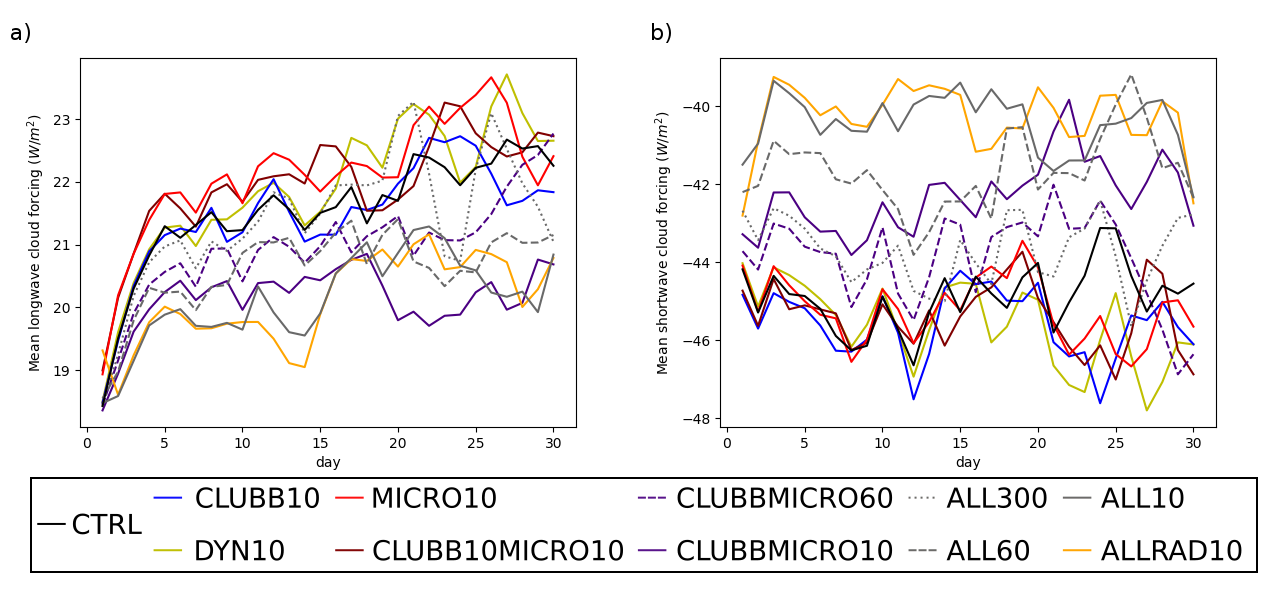
\includegraphics[width=6.5in]{Figure12.png}
    \caption[Radiative cloud forcing over time for short EAMv1 runs using different forms of substepping]{Daily global means of a) longwave cloud forcing and b) shortwave cloud forcing for substepped runs.}
    \label{fig:cld-frc}
\end{figure}

We notice that most variables take a few days for the differences between runs to fully develop, but the effect of a change in the MG2 time step strongly affects large-scale precipitation and ice water path within the first day. We suspect that most effects of a decreased time step require a certain degree of ``spin up'' in order for runs starting with the same initial condition to become more distinct. We hypothesize that the more instantaneous changes are primarily due to the direct effects of a decreased time step on microphysical process rates, which can respond directly and dramatically to changes in time step \parencite{Santos2020}.

\subsection{Substepping the ZM Deep Convection Scheme}

\label{sec:zm-substep}

So far, we have been unable to distinguish between the effect of substepping the ZM deep convection scheme and the effect of reducing the dynamics-physics coupling time step. In order to explore the effect of ZM substepping on results, we produced a simple set of code modifications to EAMv1 to allow this scheme to be substepped on its own. Most of these modifications are straightforward, since the main effect of ZM is simply to modify the state of the atmosphere for the next parameterization in the sequentially split physics. Two of ZM's outputs are precipitation process rates that are used by the modal aerosol scheme to calculate the total precipitation produced/evaporated by the deep convection. These rates are averaged over the whole time step in our modifications.

With this modified version of EAMv1, we were able to run the deep convection at a somewhat lower time step size, down to \SI{300}{\second}. However, the model becomes unstable if the ZM deep convection is a smaller time step (\SI{60}{\second} or less) while the rest of the model runs at a default time step. Specifically, the wet deposition routines in the modal aerosols behave inappropriately, causing an unphysical increase in aerosol mass due to excessive water uptake, which in turn causes the aerosol optical depth to increase exponentially until the model crashes. Even in runs that did not crash, this behavior was present and had a significant impact on model physics. We were therefore unable to investigate the effect of ZM substepping further using the model's default configuration.

Fortunately, we do have an alternative, which is to run the model with prescribed aerosols, an ability commonly used for single column runs \parencite{LebassiHabtezion2015}. This required switching to a configuration where prescribed aerosol data was available, so we used a year \num{2000} compset, FC5AV1C-04P2. As a result, these results cannot be directly compared to our previous runs, though we used the same spatial grid, and the physics of this compset is similar to our previous runs, aside from initial/boundary conditions. We reproduced the CTRL, ALL10, and CLUBBMICRO10 runs using prescribed aerosols, and further produced runs that substep ZM by itself, as well as runs that substep ZM and CLUBB+MG2 separately, and finally a run that substeps all three parameterizations. These simulations are summarized in Table \ref{tab:pa-runs}.

\begin{table}
  \centering
  \begin{tabular}{|c|p{0.3\linewidth}|r|r|}
    \hline
    Name & Substepped processes & Substep size & Run length \\
    \hline
    CTRLPA & None & N/A & \SI{30}{\day} \\
    \hline
    ALL10PA & Dynamics-physics coupling & \SI{10}{\second} & \SI{30}{\day} \\
    \hline
    CLUBBMICRO10PA & CLUBB+MG2 combined loop & \SI{10}{\second} & \SI{30}{\day} \\
    \hline
    ZM10PA & ZM deep convection & \SI{10}{\second} & \SI{30}{\day} \\
    \hline
    CLUBBMICRO10ZM10PA & CLUBB+MG2 combined loop and ZM deep convection & \SI{10}{\second} & \SI{30}{\day} \\
    \hline
    CLD10PA & CLUBB+MG2+ZM combined loop & \SI{10}{\second} & \SI{30}{\day} \\
    \hline
  \end{tabular}
  \caption{Runs performed using prescribed aerosols}
  \label{tab:pa-runs}
\end{table}

First, we note that the CLD10PA run, which substeps the ZM deep convection along with CLUBB and MG2 in a single loop, has the same effect on the partitioning of precipitation as seen in the ALL10PA run, being even closer to those results than the CLUBBMICRO10PA run was. This difference can be seen in Figure \ref{fig:precl-prect-pa}, and suggests that the reduced ZM-CLUBB-MG2 coupling time step was responsible for the increased large-scale precipitation seen in the ALL300 and ALL10 runs in Figure \ref{fig:precl-prect}. Figure \ref{fig:precl-prect-pa} also shows that substepping ZM \emph{by itself} has no effect on precipitation, since the ZM10PA run is similar to CTRLPA and the CLUBBMICRO10ZM10PA run is similar to CLUBBMICRO10PA. \textcite{Williamson2013} shows that the ZM scheme is not very active when coupled to other parameterizations at small time step sizes, when using a typical value of the convective relaxation time-scale (on the order of \num{1} hour, which is also the value in our experiments). We see the same shift from deep convection towards stratiform precipitation at short time steps.

\begin{figure}
    \centering
    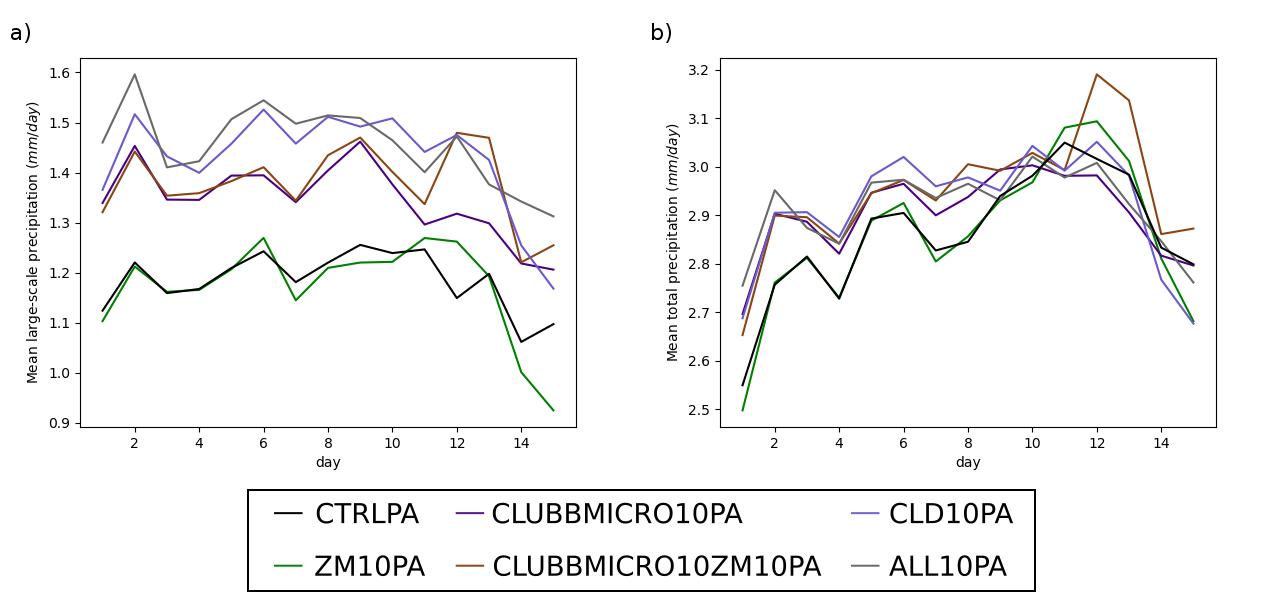
\includegraphics[width=6.5in]{Figure13.png}
    \caption[Rates of large-scale and total precipitation over time for short prescribed-aerosol EAMv1 runs using different forms of substepping]{Daily global means of a) large-scale precipitation only and b) total precipitation for prescribed aerosol substepped runs.}
    \label{fig:precl-prect-pa}
\end{figure}

In Figure \ref{fig:prec-intensity-pa}, we see that while substepping ZM may have some effect on extreme precipitation, ALL10PA still produces much heavier precipitation events than all other runs. This suggests that increasing the dynamics-physics coupling frequency is necessary to induce changes in circulation that produce these extreme events.

\begin{figure}
    \centering
    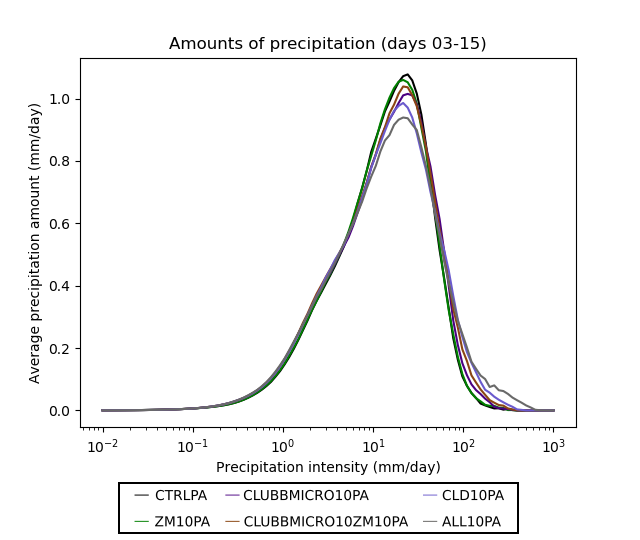
\includegraphics[width=6.5in]{PRECT_amount_d03-d15_presaer_legend.png}
    \caption[Comparison between short prescribed-aerosol EAMv1 runs with different substepping, of amount of precipitation falling as a function of intensity of precipitation events]{Global mean of the average amount of rain produced by precipitation falling at a given rate, produced from hourly data from prescribed-aerosol runs, days 3--15. Amount is normalized so that an integral over the natural logarithm of precipitation intensity yields total global mean precipitation amount.}
    \label{fig:prec-intensity-pa}
\end{figure}

Next, we note that deep convection substepping, like substepping of the other parameterizations, causes a decrease in low cloud liquid mass, and contributes to the overall pattern seen in the ALL10PA run. This is seen in Figure \ref{fig:cldliq-pa}, where the distribution of liquid water below \SI{750}{\millibar} agrees quite well between the CLD10PA run and the ALL10PA run. However, the increase in cloud liquid above this level is still absent from the CLD10PA run, implying that that increase requires more frequent dynamics-physics coupling to occur. This means that the CLD10PA ``overshoots'' the ALL10PA run in the tropics, having an even lower liquid water path. Unlike the effect of ZM substepping on precipitation, the effect on cloud liquid does not rely on coupling with CLUBB and MG2, since the CLUBBMICRO10ZM10PA run (not shown) and the CLD10PA run have fairly similar liquid water path.

\begin{figure}
    \centering
    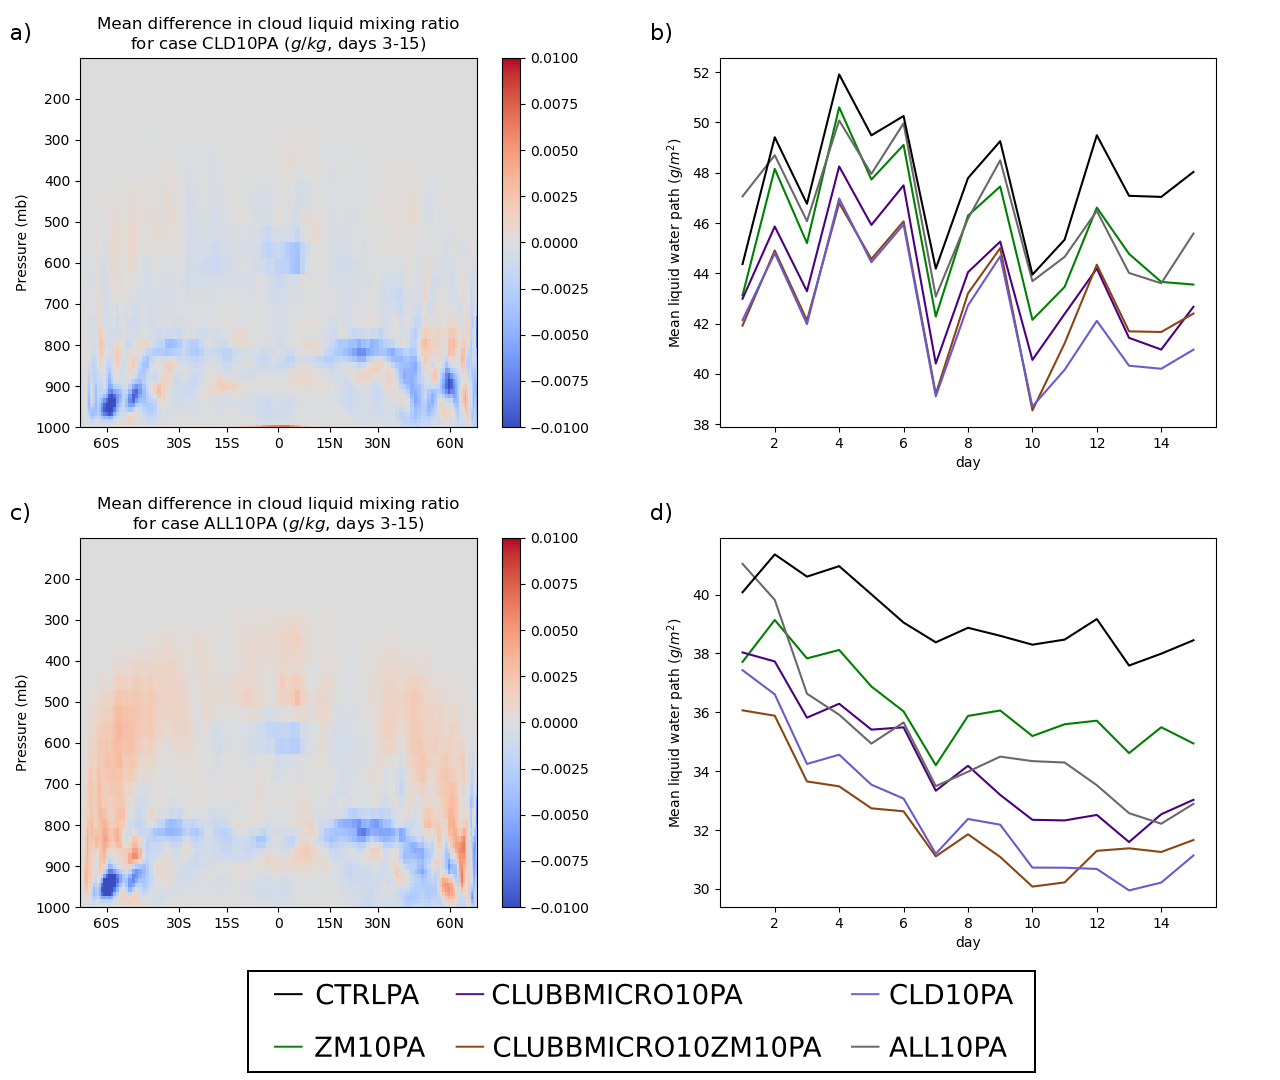
\includegraphics[width=6.5in]{Figure14.png}
    \caption[Comparison of cloud liquid mass between short prescribed-aerosol EAMv1 runs using different forms of substepping.]{Left: Differences in zonal mean cloud liquid mixing ratio versus CTRLPA for a) CLD10PA and c) ALL10PA. Right: Daily liquid water path for prescribed aerosol substepped runs using b) a global mean, and d) a mean over low latitude grid points (\num{30}S--\num{30}N).}
    \label{fig:cldliq-pa}
\end{figure}

Other than this, ZM substepping accounts for very little of the differences between the CTRLPA and ALL10PA runs. There are small decreases in cloud fraction (not shown), but these are much weaker than the effect of increased dynamics-physics coupling frequency below \SI{700}{\millibar}, and weaker than the effect of a smaller CLUBB and MG2 time step above \SI{700}{\millibar}. The effect on shortwave cloud forcing, as seen in Figure \ref{fig:cld-frc-pa}, is thus also relatively small compared with the effect of changing the CLUBB and MG2 time step. The effect of ZM substepping on longwave cloud forcing may appear to be more significant, since the CLUBBMICRO10ZM10PA run has almost the same longwave cloud forcing as the ALL10PA run. However, the mechanism here is completely different; all runs where ZM is substepped, including CLUBBMICRO10ZM10PA, have a dramatically lowered ice water path (not shown). ALL10PA and CLUBBMICRO10PA, on the other hand, have an ice water path similar to the control, and so the decrease in longwave cloud forcing is instead attributable to decreased cloud fraction in these cases.

\begin{figure}
    \centering
    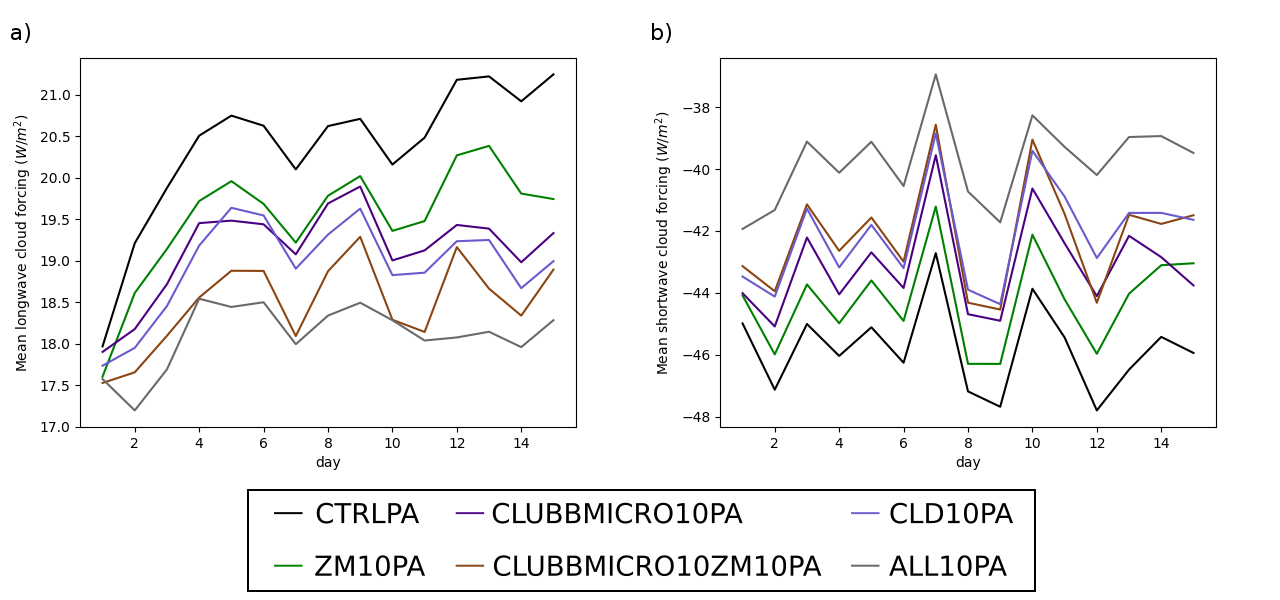
\includegraphics[width=6.5in]{Figure15.png}
    \caption[Radiative cloud forcing over time for short prescribed-aerosol EAMv1 runs using different forms of substepping]{Daily global means of a) longwave cloud forcing and b) shortwave cloud forcing for prescribed aerosol substepped runs.}
    \label{fig:cld-frc-pa}
\end{figure}

\section{Discussion} \label{sec:EAM-discussion}

EAMv1 at its default \SI{1800}{\second} time step produces very different results from the same model at a \SI{10}{\second} time step, indicating that the release implementation should not be viewed as calculating the ``time-resolved'' solution to the system of equations that defines the model physics. The amount and regional distribution of precipitation, and especially the radiatively-important partitioning between large-scale and convective precipitation, shows particularly strong sensitivity to the time step size. The cloud radiative forcings also differ by several watts per square meter, indicating that a reduction in the time step would require, at a minimum, significant retuning of the model to produce reasonable results. By experimenting with substepping of model components, we have been able to distinguish three main model time steps that account for most of the changes seen between the \SI{1800}{\second} and \SI{10}{\second} versions of the model.

First, a reduction of the combined CLUBB and MG2 time step causes the following changes:

\begin{enumerate}
    \item An increase in total precipitation, leading to a reduction in humidity and a reduction in cloud liquid mass below \SI{750}{\millibar}.
    \item A reduction in the ratio of convective to large-scale precipitation.
    \item Regional changes in precipitation, most notably including a massive increase in average precipitation on the maritime continent and in South America.
    \item A reduction in cloud fraction above \SI{700}{\millibar}, causing a large reduction in the magnitudes of both shortwave and longwave radiative cloud forcing.
\end{enumerate}

A much smaller increase in large-scale precipitation can be produced by changing the time step for MG2 alone, but otherwise these effects are only seen when CLUBB and MG2 are substepped together.

Second, a reduction of the dynamics-physics coupling time step (a.k.a. dtime) causes the following changes:

\begin{enumerate}
    \item An increase in cloud mass in the upper troposphere, especially in the midlatitudes.
    \item A substantial decrease in cloud fraction below \SI{700}{\millibar}, causing further large decreases in radiative cloud forcing, especially for shortwave radiation.
\end{enumerate}

Third, a reduction of the ZM time step causes the following changes:

\begin{enumerate}
    \item A further reduction in cloud liquid mass below \SI{750}{\millibar}.
    \item A small decrease in cloud fraction everywhere, causing further small decreases in radiative forcings.
    \item A further reduction in the ratio of convective to large-scale precipitation. (However, this only occurs when ZM is coupled more frequently with CLUBB and MG2, which in the original code can only be done by reducing dtime.)
\end{enumerate}

In addition to these effects, we also find that substepping individual parameterizations can cause strong effects on ice water path (and consequently on longwave cloud forcing). Ice water path increases substantially if MG2 is substepped independently from CLUBB, but not if MG2 is substepped together with CLUBB. Similarly, ice water path decreases if ZM is substepped, especially if it is substepped independently of CLUBB and MG2. Each of these effects are an order of magnitude larger than the overall difference in ice water path seen between ALL10 and the CTRL. This means that substepping either ZM or MG2 individually can introduce large numerical biases, and produce a much worse approximation to the resolved cloud ice physics than would be produced by the default settings.

These observations indicate that the time step sensitivity of a full climate model cannot be regarded as simply the sum of the effects that come from substepping each individual parameterization alone. Coupling frequencies between related processes can independently cause time step sensitivity. Nonetheless, it is possible to attribute the time step sensitivity of some variables to particular processes or sets of processes. The implications of these facts for model development may be underappreciated, since developers of new parameterizations tend to focus on the time step of their own particular physics packages, rather than the frequency with which they are coupled to other parts of a model. In our study, substepping CLUBB alone has no discernible effect on model climate, yet sensitivity to the coupling frequencies between CLUBB and other processes is arguably the most important form of time step sensitivity in EAMv1.

\chapter{Conclusions} \label{ch:conclusions}

This chapter summarizes our results and discusses their implications for future studies.

\section{Summary of Results} \label{sec:summary}

We have examined the time step sensitivity of EAMv1 from two different perspectives. First, we used a ``bottom-up'' approach, focusing on the MG2 cloud microphysics parameterization, which we believed was an important factor affecting EAMv1's time step sensitivity. Using a data set of typical MG2 inputs from EAMv1, we numerically calculated the eigenvalues of the Jacobian of MG2's processes, and thus obtained a set of timescales associated with MG2 as it typically operates in EAMv1. We found that these timescales could be heuristically associated with particular processes and combinations of processes.

By experimenting with substepping particular processes within MG2, we were able to show that, in some regimes, our analysis successfully identified both the maximum time steps that could resolve the model's trajectory, and sets of coupled processes that could be substepped to produce similar results without reducing the overall MG2 time step. However, we also found that, in other regimes, the nonlinearity in the physics played a large enough role within a single \SI{300}{\second} time step to frustrate our approach, which was based on linear stability analysis.

We then used a ``top-down'' approach, where we reduced the time step of the entire EAMv1 physics to gain a broad understanding of time step sensitivity in the model. We find that reducing the EAMv1 time step produces large changes in model climate, comparable to the effect of halving horizontal resolution. Our findings match prior literature on the time step sensitivity of precipitation in GCMs. However, EAMv1 and SPCAM3 experience decreases in precipitable water and lowered cloud fraction at short time step sizes, while CAM3 experiences an increase in both variables. This shows that time step sensitivity has different impacts on GCMs with different cloud physics parameterizations.

To attribute this time step sensitivity to particular processes, we performed a series of experiments reducing the time steps of different physics packages independently from one another. This allowed us to experimentally determine which packages needed to be substepped to best replicate the effects of reducing the whole model time step. We identified three main time steps within the model, which together account for most of the overall time step sensitivity of EAMv1:

\begin{enumerate}
    \item The time step used to jointly substep CLUBB and MG2.
    \item The time step at which the dynamics-physics coupling occurs.
    \item The time step used by the ZM deep convection.
\end{enumerate}

Across our studies, we consistently found that the coupling between processes is a major contributor to the time step sensitivity of climate models, and in many cases is more important than the time steps used by individual parameterizations. We conclude that it is generally not possible to understand the time step sensitivity of climate models by examining each particular process independently. While substepping is a common method of improving time integration of specific processes, we cannot assume that it will be effective in reducing the time integration error in the overall model unless we have accounted for interactions between processes.

\section{What Now?} \label{sec:future}

It appears that EAMv1 suffers from a significant flaw, one likely present in the atmospheric components of most climate models. On the one hand, considerable human effort is put into inventing new equations to parameterize atmospheric physics, and to implement those equations in code. Huge resource allocations at high performance computing centers are then allotted to running the model for simulated centuries or millennia. On the other hand, EAMv1's physics packages are clearly failing to accurately integrate the equations they purport to solve at the default time step. When the representation of a process in the model is complex and expensive, yet also not accurate at the default time step, we are left with two possibilities. If resolving that process is important for studying climate, the model is not producing the results that researchers need. If that process is not important, we are probably wasting a significant amount of resources on a sophisticated parameterization when a cruder approximation would suffice.\footnote{The climate modeling community has been dealing with a similar dilemma with respect to horizontal resolution. This has led to the development of higher resolution models for studies where the extra resolution is needed, including the \ang{0.25} configuration of EAMv1 itself. There has also been an increased interest in regionally refined grids, where the horizontal grid spacing is reduced over regions of particular interest for a given study. However, temporal resolution has not received the same amount of attention, even though (as we have shown) using a shorter time step at a \ang{1} resolution can change model climate just as much as changing the horizontal grid spacing.}

In order to repair this flaw, we need to figure out which processes are most in need of improved time integration. This study has already demonstrated that certain physics packages are responsible for most of EAMv1's time step sensitivity, and introduced some techniques that may be useful for attributing time step sensitivity to particular processes in the future. This research could be extended by performing further runs with short time steps, for the purpose of examining specific known biases in EAMv1 and determining whether these biases are related to time integration error.

Alternatively, one could explore broader questions with short time step runs, such as whether changes to EAMv1's time step affects the model's response to climate change. Equilibrium climate sensitivity is not consistent across climate models, leading to significant uncertainty about the long-term direction of climate change. Historically, the shortwave low cloud feedback has been a major source of this uncertainty \parencite{Bony2005,Andrews2012,Zelinka2020}. It would therefore be reasonable to compare a model running at a long time step to the same model tuned to produce a similar present day climate at a short time step, assessing whether the equilibrium climate sensitivity depends strongly on time step.

If the time step sensitivity in EAMv1 does need to be addressed to improve the model's accuracy, we are left in need of a set of strategies to improve time integration when simply reducing the time step on small parts of the code is inadequate. In particular, the dynamics-physics coupling frequency affects the entire model, and the CLUBB-MG2 coupling frequency affects two parameterizations that account for a large fraction of EAMv1's cost.

It may be possible to improve the dynamics-physics coupling by simply reducing the time step, as in the ALL300 run from chapter \ref{ch:EAM}. Most calculations in the dynamics and many physics parameterizations are already running at a five minute time step or less, even for lower resolution runs. \textcite{Donahue2020} found that for a \ang{1}~simulation, halving the dynamics-physics coupling frequency only increased model cost by \SI{20}{\percent}. Our ALL300 run had one-sixth the physics time step of the CTRL run, but only required \SI{66}{\percent} more core-hours per simulated year. It is not free to increase the coupling frequency by a factor of six, but not even doubling the computational cost makes this a bargain.

Alternatively, it may be possible to make further changes to the dynamics-physics coupling to simulate more frequent interaction without requiring direct dynamics-physics interaction. In \textcite{Wan2020}, a pre-publication study using methods similar to chapter \ref{ch:EAM} of this paper, the authors experiment with using the ``dribbling'' method to couple all other processes (including the dynamics) to the CLUBB and MG2 loop, in the same way as all physics processes are dribbled into the model's dynamical core. While a detailed discussion of this experiment is not yet available, the effect of implementing this method on cloud radiative effect resembles the effect of increasing the dynamics-physics coupling frequency.

The sensitivity to CLUBB-MG2 coupling is more difficult to address. We cannot reduce time integration error much by substepping either CLUBB or MG2 alone, and CLUBB and MG2 together account for a large share of the model cost. Furthermore, many of the timescales we found associated with MG2 are on the order of \SI{10}{\second}, but reducing the CLUBB and MG2 combined time step by a factor of \num{30} could slow down EAMv1 by an order of magnitude compared to the default configuration. Most modelers will not be able to accept such a large increase in computational cost, but we can suggest a few other ways of working around this cost in future model development:

\begin{enumerate}
    \item Reduce the cost of simulating the most expensive aspects of a process, e.g. by switching to simpler implementations manually, or using machine learning to produce a cheap approximation to approximate process rates. A parameterization that uses a less accurate approximation for some process, but is cheap enough to run at a higher temporal or spatial resolution, may end up being more accurate than a parameterization that uses a more accurate set of equations.
    \item Use alternative time integration schemes (e.g. changing the operator splitting, using higher-order methods) to lower the time integration error at moderate time step sizes.
    \item Redesign the physics to separate out processes that have a shorter or longer time scale. This would mean refactoring CLUBB and MG2 (or any future set of schemes that cause similar issues), in order to isolate the parts of those parameterizations that are most responsible for the time step sensitivity of the overall model. If this subset of physical processes can be calculated much more cheaply than the total cost of CLUBB and MG2, it could then be handled with a more accurate time integration scheme without incurring an excessive cost.
\end{enumerate}

We will conclude by briefly returning to the subject of MG2's rain evaporation, to demonstrate that even fairly simple changes along these lines can have beneficial effects. We found in \ref{sec:MG2-impact} that the rain evaporation and rain self-collection must be substepped together in order to produce an accurate rain evaporation rate (Figure \ref{convergence-evap-scol}). Long afterward, we returned to this problem to see what effect a sequential split would have on the error. These new results are shown in Figure \ref{fig:convergence-splitting}.

\begin{figure}[htbp]
  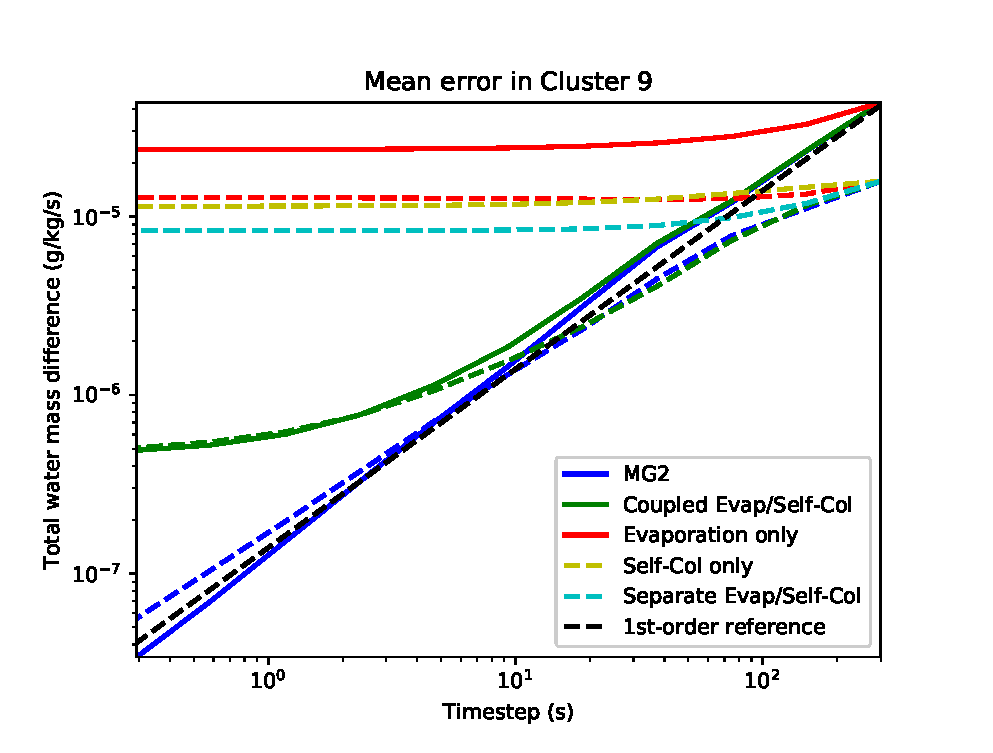
\includegraphics[width=6.5in]{substep_convergence_mean_seq_c9_richext.eps}
  \caption[Convergence plot for mean MG2 error in a cluster of rainy, cloudless grid cells using different splitting and substepping strategies]{Convergence plot for mean error in cluster 9 grid cells under different splitting and substepping strategies for rain evaporation and self-collection. Runs substepping all of MG2 are shown in blue. Runs substepping evaporation and self-collection together are shown in green. Runs substepping evaporation alone shown in red. Runs substepping self-collection alone shown in yellow. Runs substepping self-collection and evaporation in separate loops shown in cyan. All non-substepped processes run at \SI{300}{\second}. Solid colors use parallel splitting for all processes, while dashed lines use sequential splitting to run self-collection before evaporation, with all other processes in parallel. The dotted reference line has slope \num{1}. The reference state is derived using Richardson extrapolation from the two shortest runs substepping all of MG2 using parallel splitting.}
  \label{fig:convergence-splitting}
\end{figure}

In our earlier parallel splitting results (solid), substepping all of MG2 (blue) led to roughly first-order convergence. Substepping rain evaporation and self-collection (green) also produced roughly first-order convergence down to about \SI{10}{\second}, though at smaller time steps the error was increasingly dominated by processes we were not substepping (mainly accretion). Substepping the evaporation alone (red) could only reduce the error by less than a factor of two.

We find that all of this is also true for the sequential splitting (dashed), but with a lower error at large time steps. Using sequential splitting, we can also see what happens when we substep self-collection in a separate loop either before taking a single large evaporation step (yellow), or before taking an equal number of evaporation substeps (cyan). The latter strategy produces a lower error than substepping the evaporation alone, but neither converges to a low-error result. This again shows the importance of coupling between the two processes; the only difference between the coupled substepping sequential method (dashed green) and the separate substepping sequential method (dashed cyan) is that the former alternates between the two processes rather than performing all self-collection steps before all rain evaporation steps.

Using sequential splitting at the $\SI{300}{\second}$ default time step allows the rain self-collection to grow rain particles before the evaporation is calculated, producing a smaller evaporation rate than we get from parallel splitting. This the reduces overall error by about a factor of three. This does not mean the processes are well resolved at the default time step. Even using sequential splitting, the magnitude of the error is still fairly large, and the rate of convergence is below first-order. Nonetheless, the error is significantly reduced by using a sequential split, and this improvement requires only a few lines of code and adds almost nothing to the computational cost of MG2. Additional tweaks to the splitting method (Strang splitting?) would likely yield further improvements.

In this study, we have found that we can not generally deal with time step sensitivity in a climate model by simply substepping whichever atmospheric processes produce the largest time integration errors. However, this is not as much of an obstacle than it might seem. If we study a climate model's time step sensitivity and attribute that sensitivity to a subset of its physical processes, we have a range of options available to us to improve its overall time-differencing accuracy. Many of the flaws and potential pitfalls in EAMv1 time integration can be done away with, if we simply take the time to identify and target the specific physical processes responsible.

\printendnotes

%
% ==========   Bibliography
%
%\nocite{*}   % include everything in the uwthesis.bib file
%\bibliographystyle{plain}
\printbibliography[heading=bibintoc]
%
% ==========   Appendices
%
\appendix
\raggedbottom\sloppy
 
% ========== Appendix A
 
\chapter{Archived Code and Data Used in this Study}

The data used for chapter \ref{ch:MG2} is available at the following URL, using Argonne National Laboratory's Petrel service: \url{https://dabdceba-6d04-11e5-ba46-22000b92c6ec.e.globus.org/publications/Santos_JAMES_2019.tar}. The TAR archive at this location contains the following files:
\begin{enumerate}
    \item MG2\_data\_collection.cam.h1.0001‐01‐06‐00000.nc --- Data set used to provide inputs to MG2.
    \item MG2\_data\_collection.10\_cluster\_labels.0001‐01‐06‐00000.nc --- Labels input grid points according to clusters generated via k‐means.
    \item Jacobian\_cutoff\_* --- Eigenvalues derived from the numerical derivative of MG2 for each grid point. These were calculated in parallel and placed in 12 separate files.
    \item nsubr\_control\_ANN\_climo.nc --- Averaged data from control run used for Figures \ref{e3sm-taylor}-\ref{e3sm-rain-comparison}.
    \item short\_time step\_ANN\_climo.nc --- Averaged data from short MG2 time step run used for Figures \ref{e3sm-taylor}-\ref{e3sm-rain-comparison}.
\end{enumerate}

The code for chapter \ref{ch:MG2} is available on GitHub at \url{https://github.com/quantheory/mg2-python-driver/tree/thesis-v1}, or as doi:10.5281/zenodo.4287596.

The data used for chapter \ref{ch:EAM} is still being prepared for archival. When this process is complete, information about this data will accompany the final version of \cite{Santos2020}. The raw data (a compressed tarball about \SI{433}{\giga\byte} in size) is also available at \url{https://drive.google.com/file/d/1yENgyLnaUNBGhEMMx0u6vbivk5lcqDMC/view?usp=sharing}. The code for Chapter \ref{ch:EAM} is available on GitHub at \url{https://github.com/quantheory/E3SMTimestepStudy/tree/thesis-v1}, or as doi:10.5281/zenodo.4287611.

\end{document}
